\chapter{Экспериментальные исследования}\label{ch:ch4}

\section{Проведение измерений}

Для экспериментальной проверки достоверности разработанной методики и анализа остаточного реактивного момента была проведена серия стендовых испытаний. Целью экспериментов являлась регистрация динамических характеристик МНО и сопоставление полученных данных с расчётными значениями, приведёнными во 2-й главе.

Перед началом испытаний МНО была установлена в кантователь стенда, так, чтобы ось $Z$ изделия была совмещена с осью чувствительности стенда. Для исключения влияния внешних факторов проводилась юстировка подвесной системы. Центр карданова подвеса совмещался с центром масс подвижной части каркаса, что контролировалось с использованием уровня и регулируемого зацепа подвесных струн. Расположение МНО в стенде представлено на рисунке~\cref{fig:yoim-omn}

\begin{figure}[h!]
	\centering
	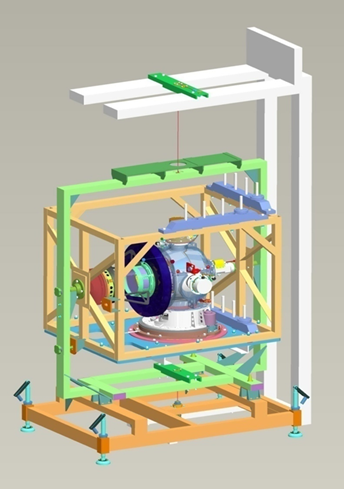
\includegraphics[scale=0.8]{images/yoim-omn}
	\caption{Размещение МНО в составе измерительного стенда}
	\label{fig:yoim-omn}
\end{figure}

Дополнительно проверялась работоспособность средств измерений. Волоконно-оптический гироскоп проходил контроль по регистрации проекции угловой скорости вращения Земли; допустимое расхождение с расчётным значением не превышало 0,3 \%, что подтверждало готовность прибора к измерениям. Включение электронной аппаратуры осуществлялось за 30 минут до начала эксперимента для обеспечения термостабилизации.

Условия окружающей среды контролировались согласно методике, описанной в главе 3. Температура поддерживалась в пределах 20–23 °C, относительная влажность — около 50 \%, атмосферное давление фиксировалось барометром-анероидом. Таким образом исключалось влияние климатических факторов на стабильность работы гироскопа и привода.

В качестве опорного воздействия задавался серия тестовых воздействий величиной $M_{\text{тест}} = \SI{0,005}{\newton\meter}$. При этом отклик подвеса регистрировался гироскопом по угловой скорости колебаний. Скорость колебаний показана на рисунке~\cref{fig:test-gyro}.

\begin{figure}[h!]
	\centering
	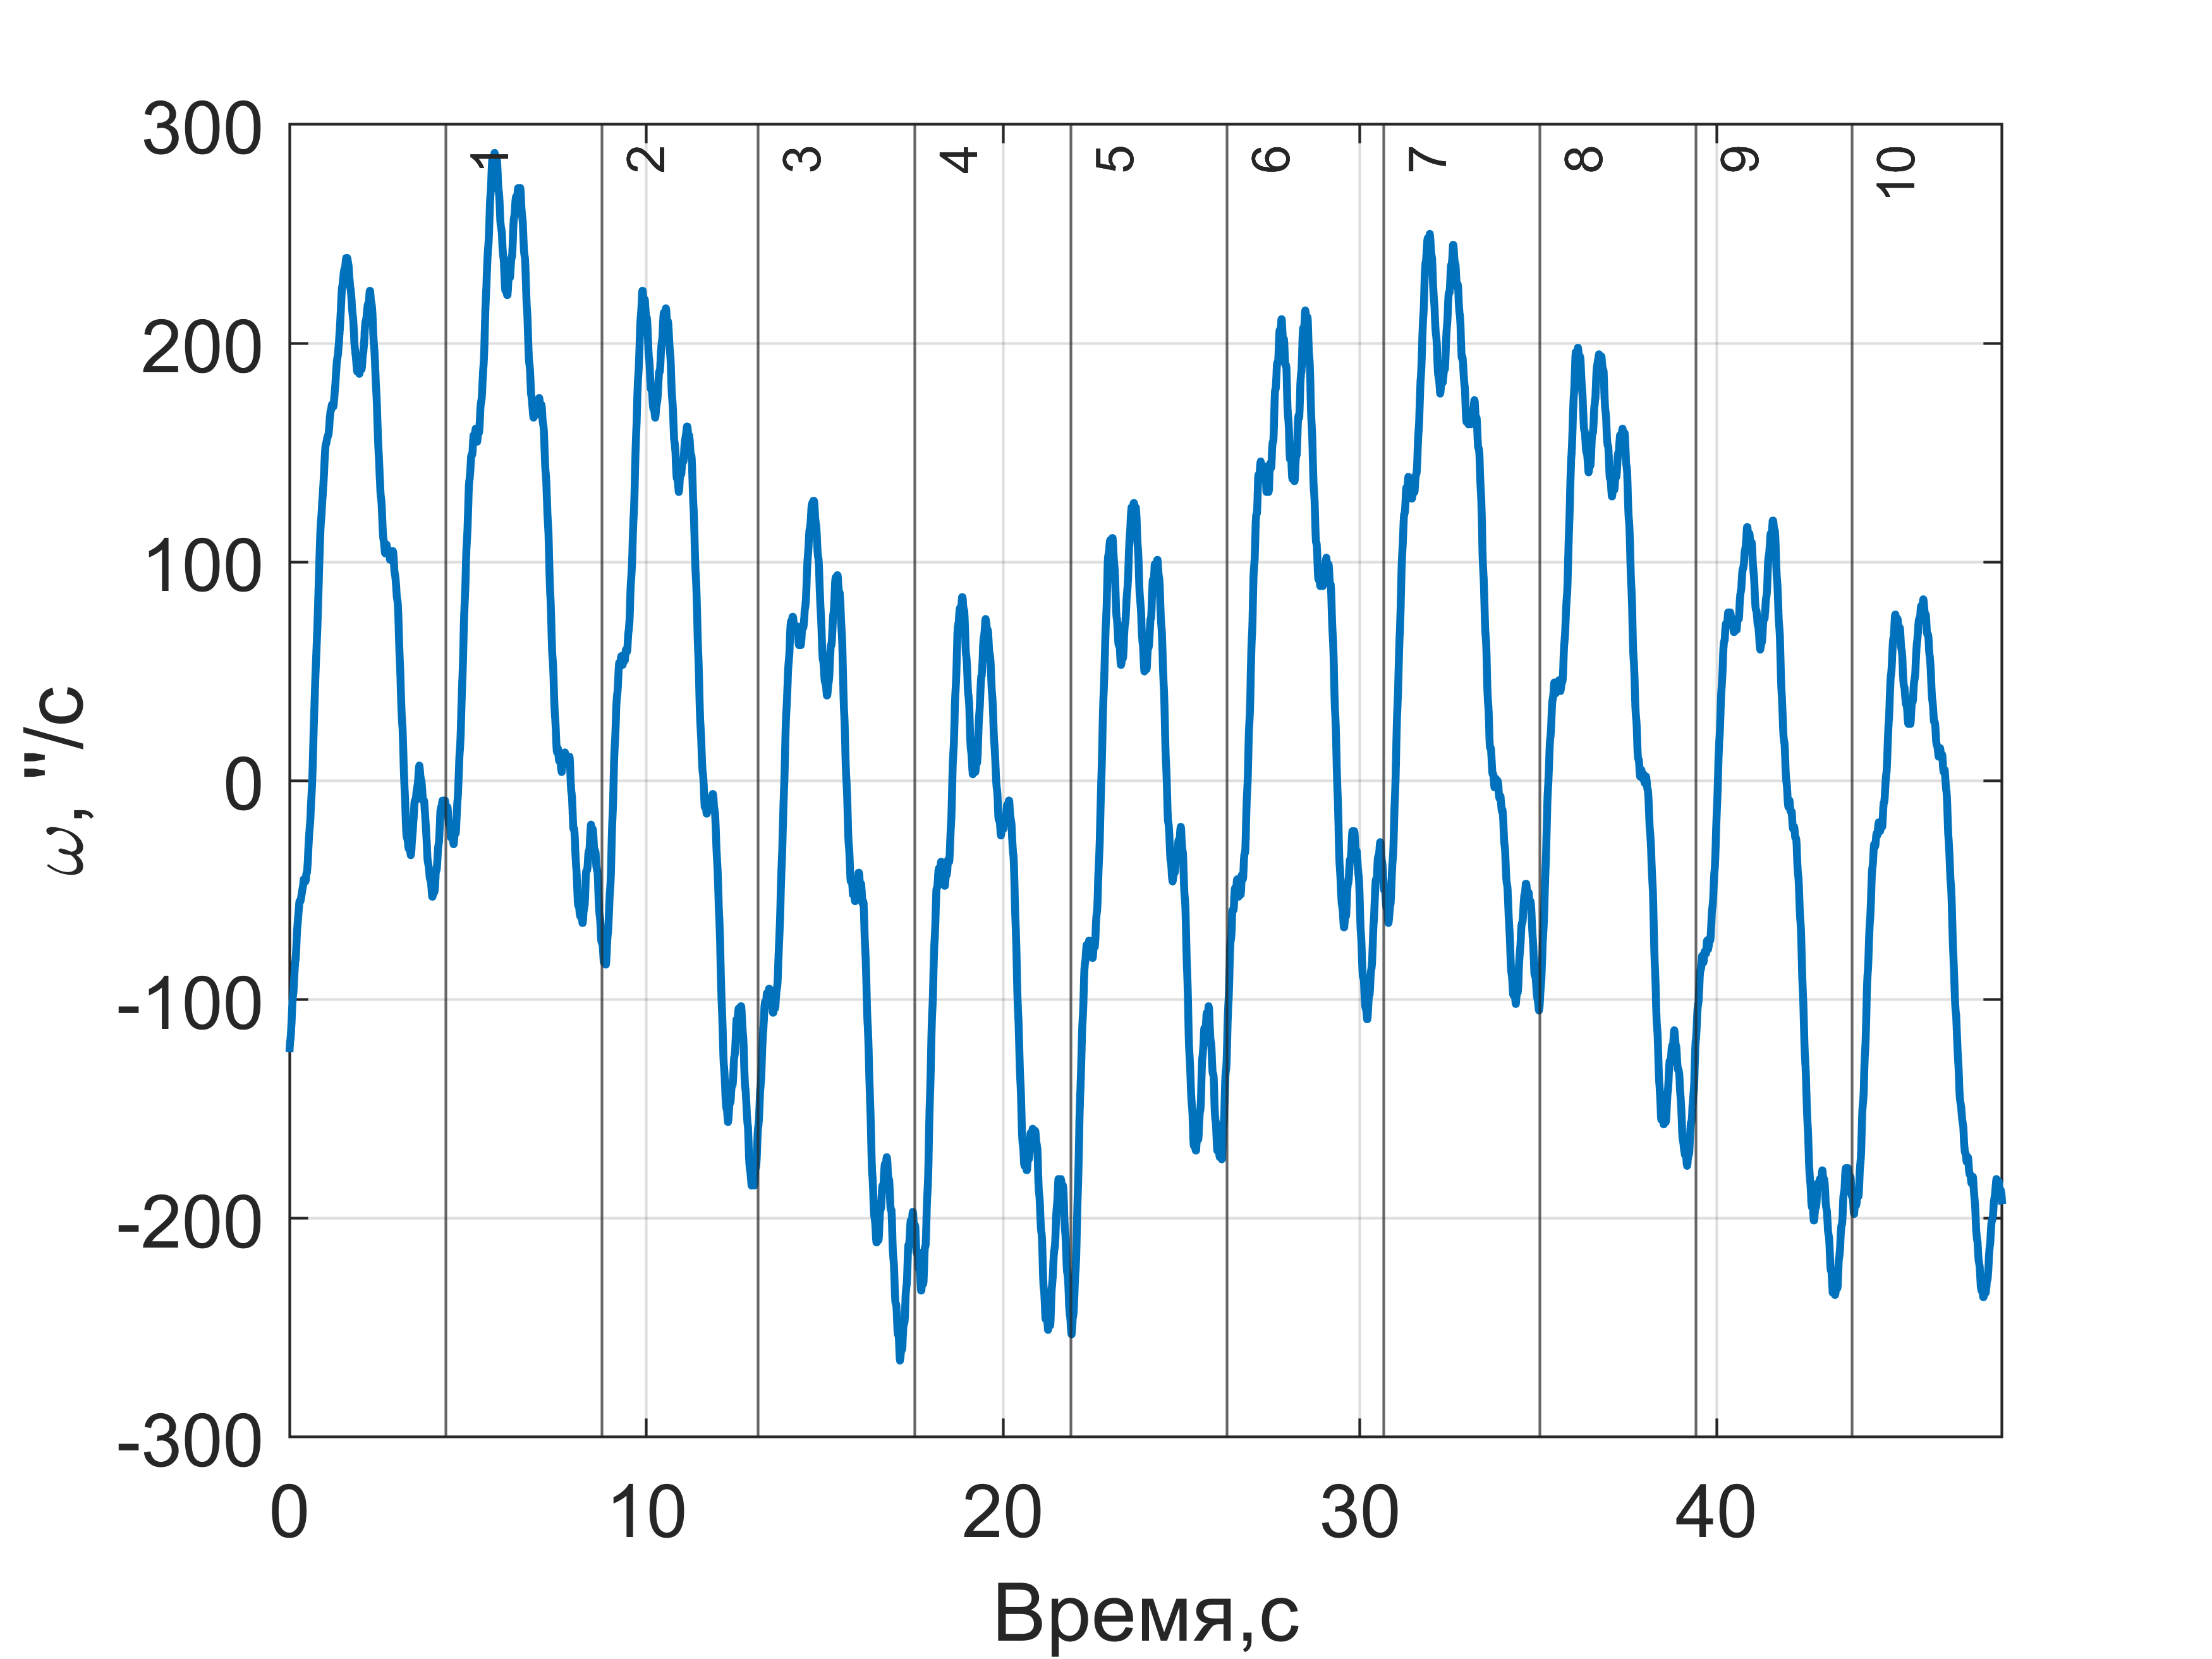
\includegraphics[scale=0.8]{matlab/img/test-gyro}
	\caption{Угловая скорость колебаний стенда при серии тестовых воздействий}
	\label{fig:test-gyro}
\end{figure}

Зарегистрированные временные зависимости угловой скорости подвергались предварительной обработке: полученные временные ряды были приведены к единой временной шкале и усреднены по ансамблю реализаций Такой подход позволил подавить случайные шумы гироскопа и выделить характерный отклик системы на заданный момент $M_{\text{тест}}$. В результате формировалась усреднённая кривая угловой скорости (Рисунок~\cref{fig:test-gyro-sum}), которая использовалась в дальнейшем как эталон для сравнения с экспериментами при перенацеливании МНО.

\begin{figure}[h!]
	\centering
	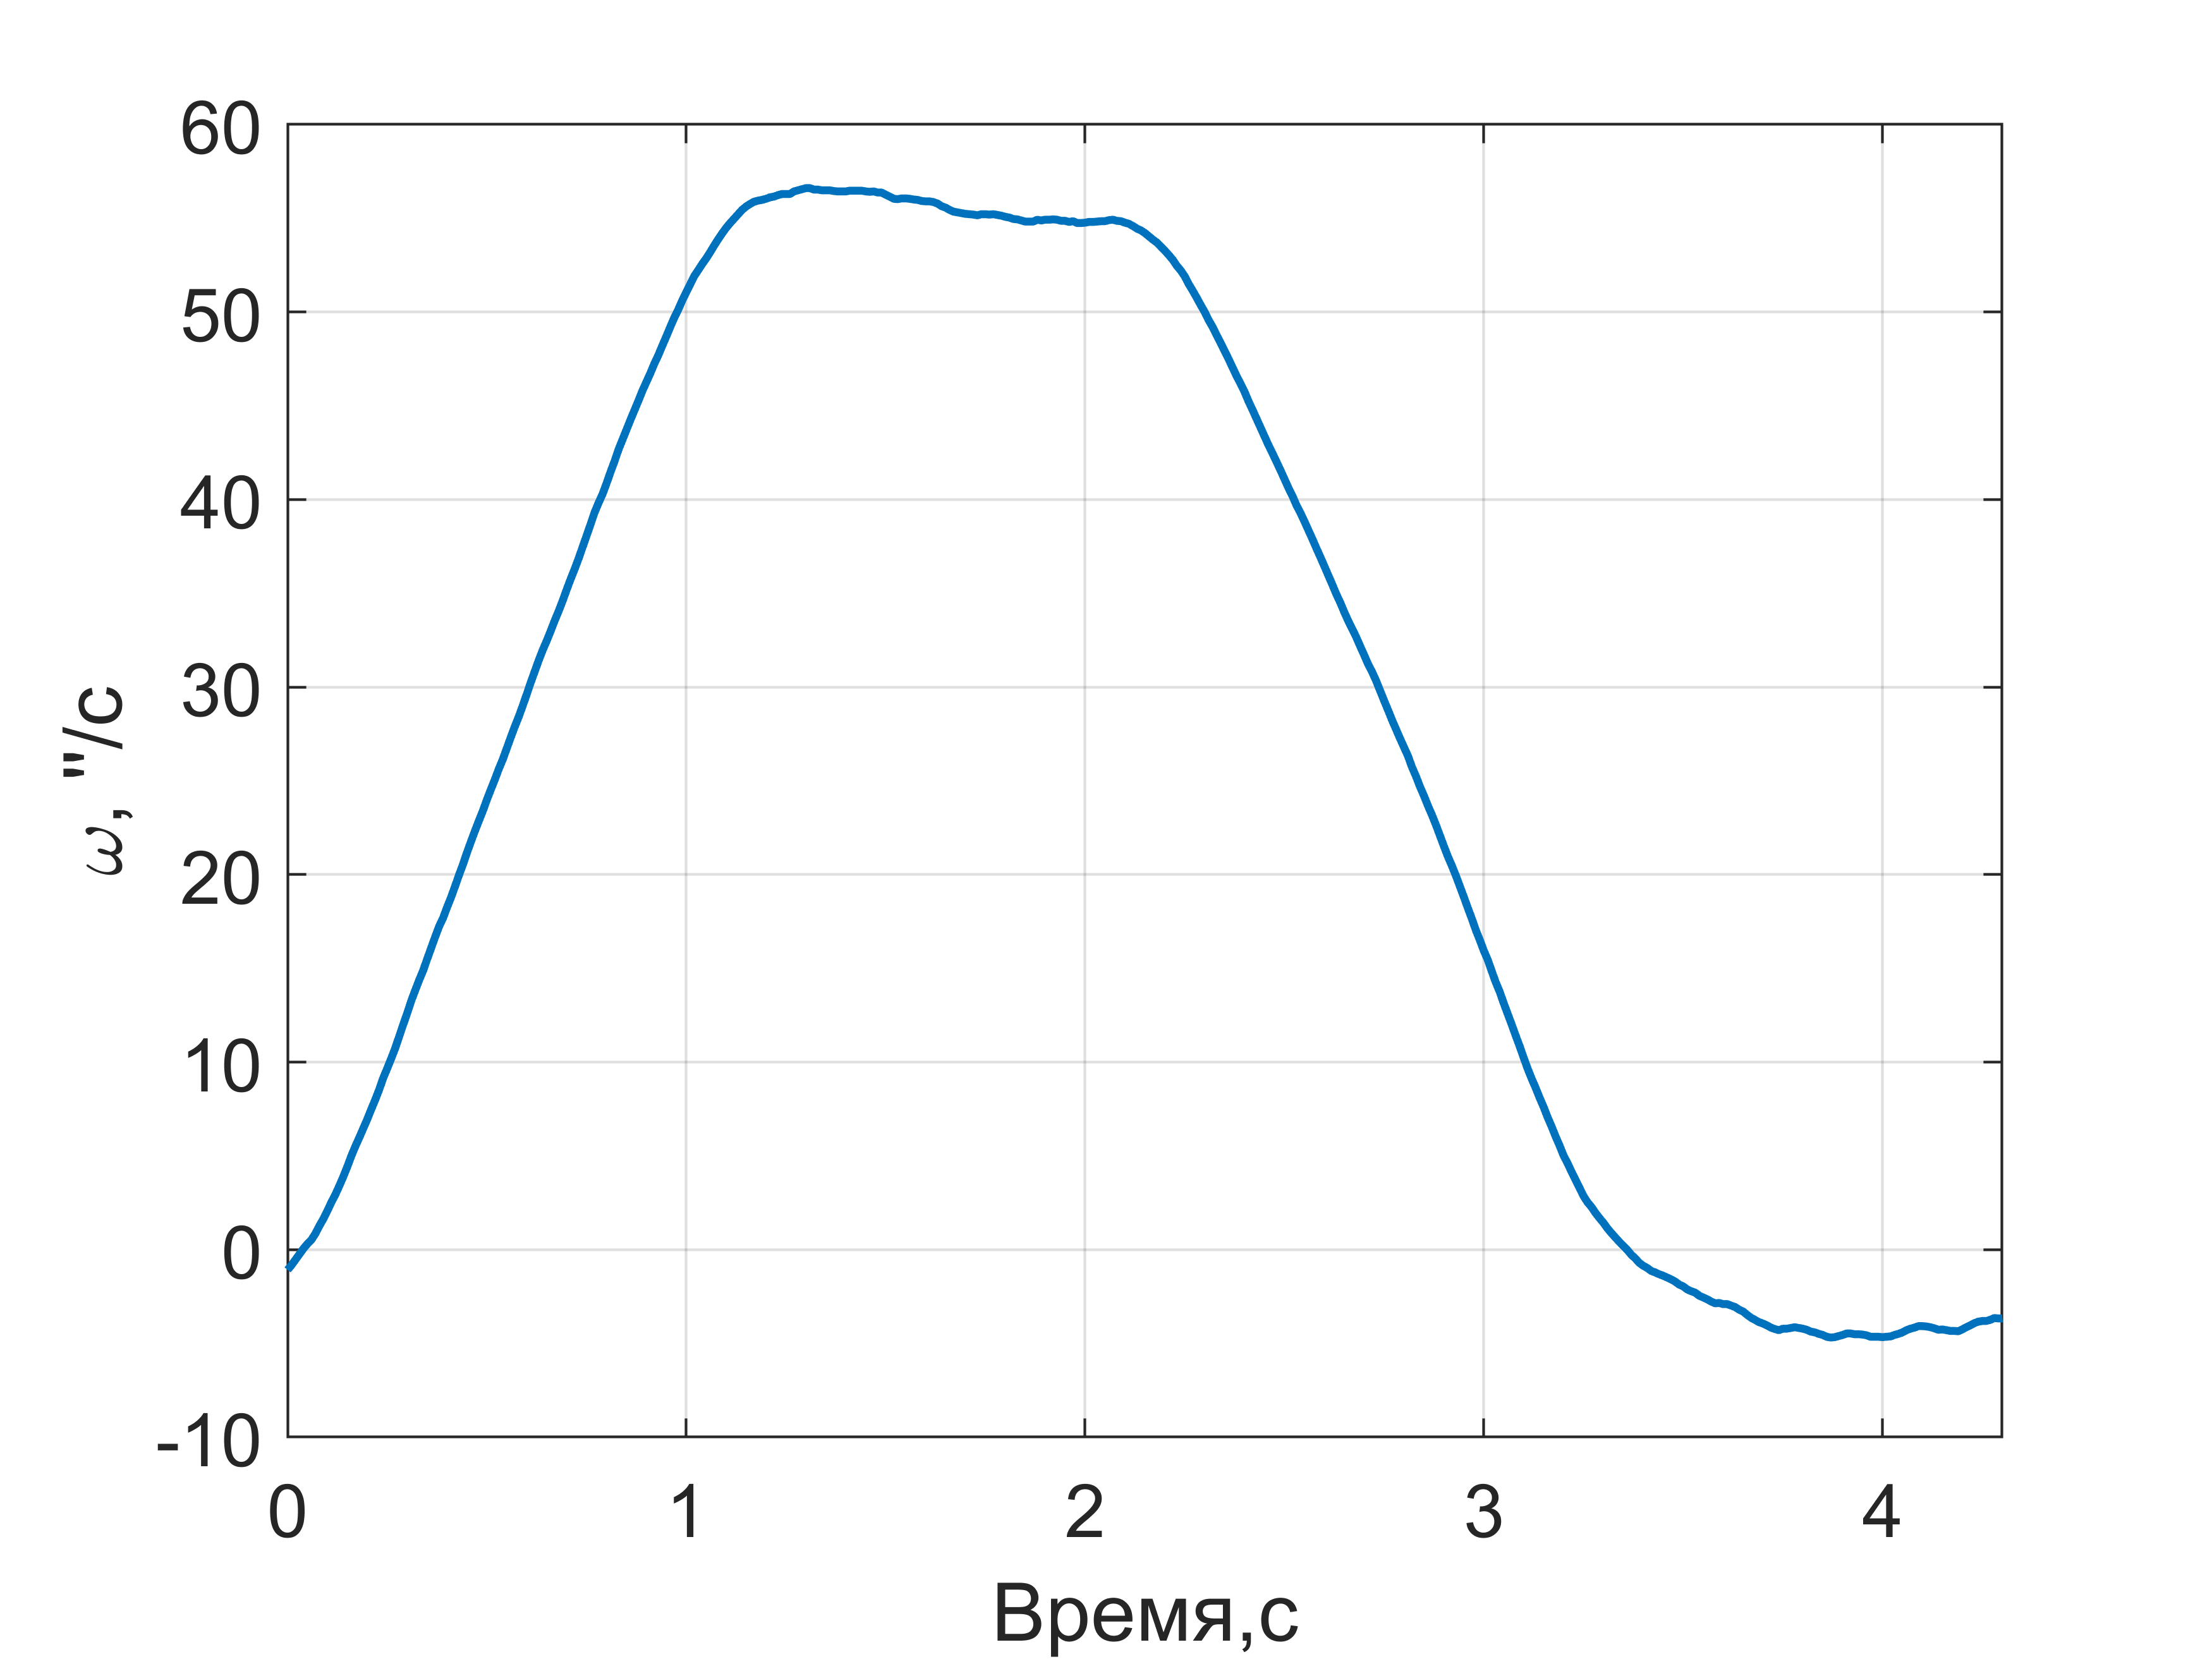
\includegraphics[scale=0.8]{matlab/img/test-gyro-sum}
	\caption{Усреднённая угловая скорость колебаний стенда при серии тестовых воздействий}
	\label{fig:test-gyro-sum}
\end{figure}

Для дальнейшего анализа усреднённый сигнал угловой скорости $\omega(t)$ был подвергунт численному дифференцированию. В результате определялась временная зависимость углового ускорения $\epsilon(t)$, которое характеризует динамическую реакцию стенда на приложенный момент. 
На рисунке~\cref{fig:test-gyro-acc} представлена временная зависимость углового ускорения.

\begin{figure}[h!]
	\centering
	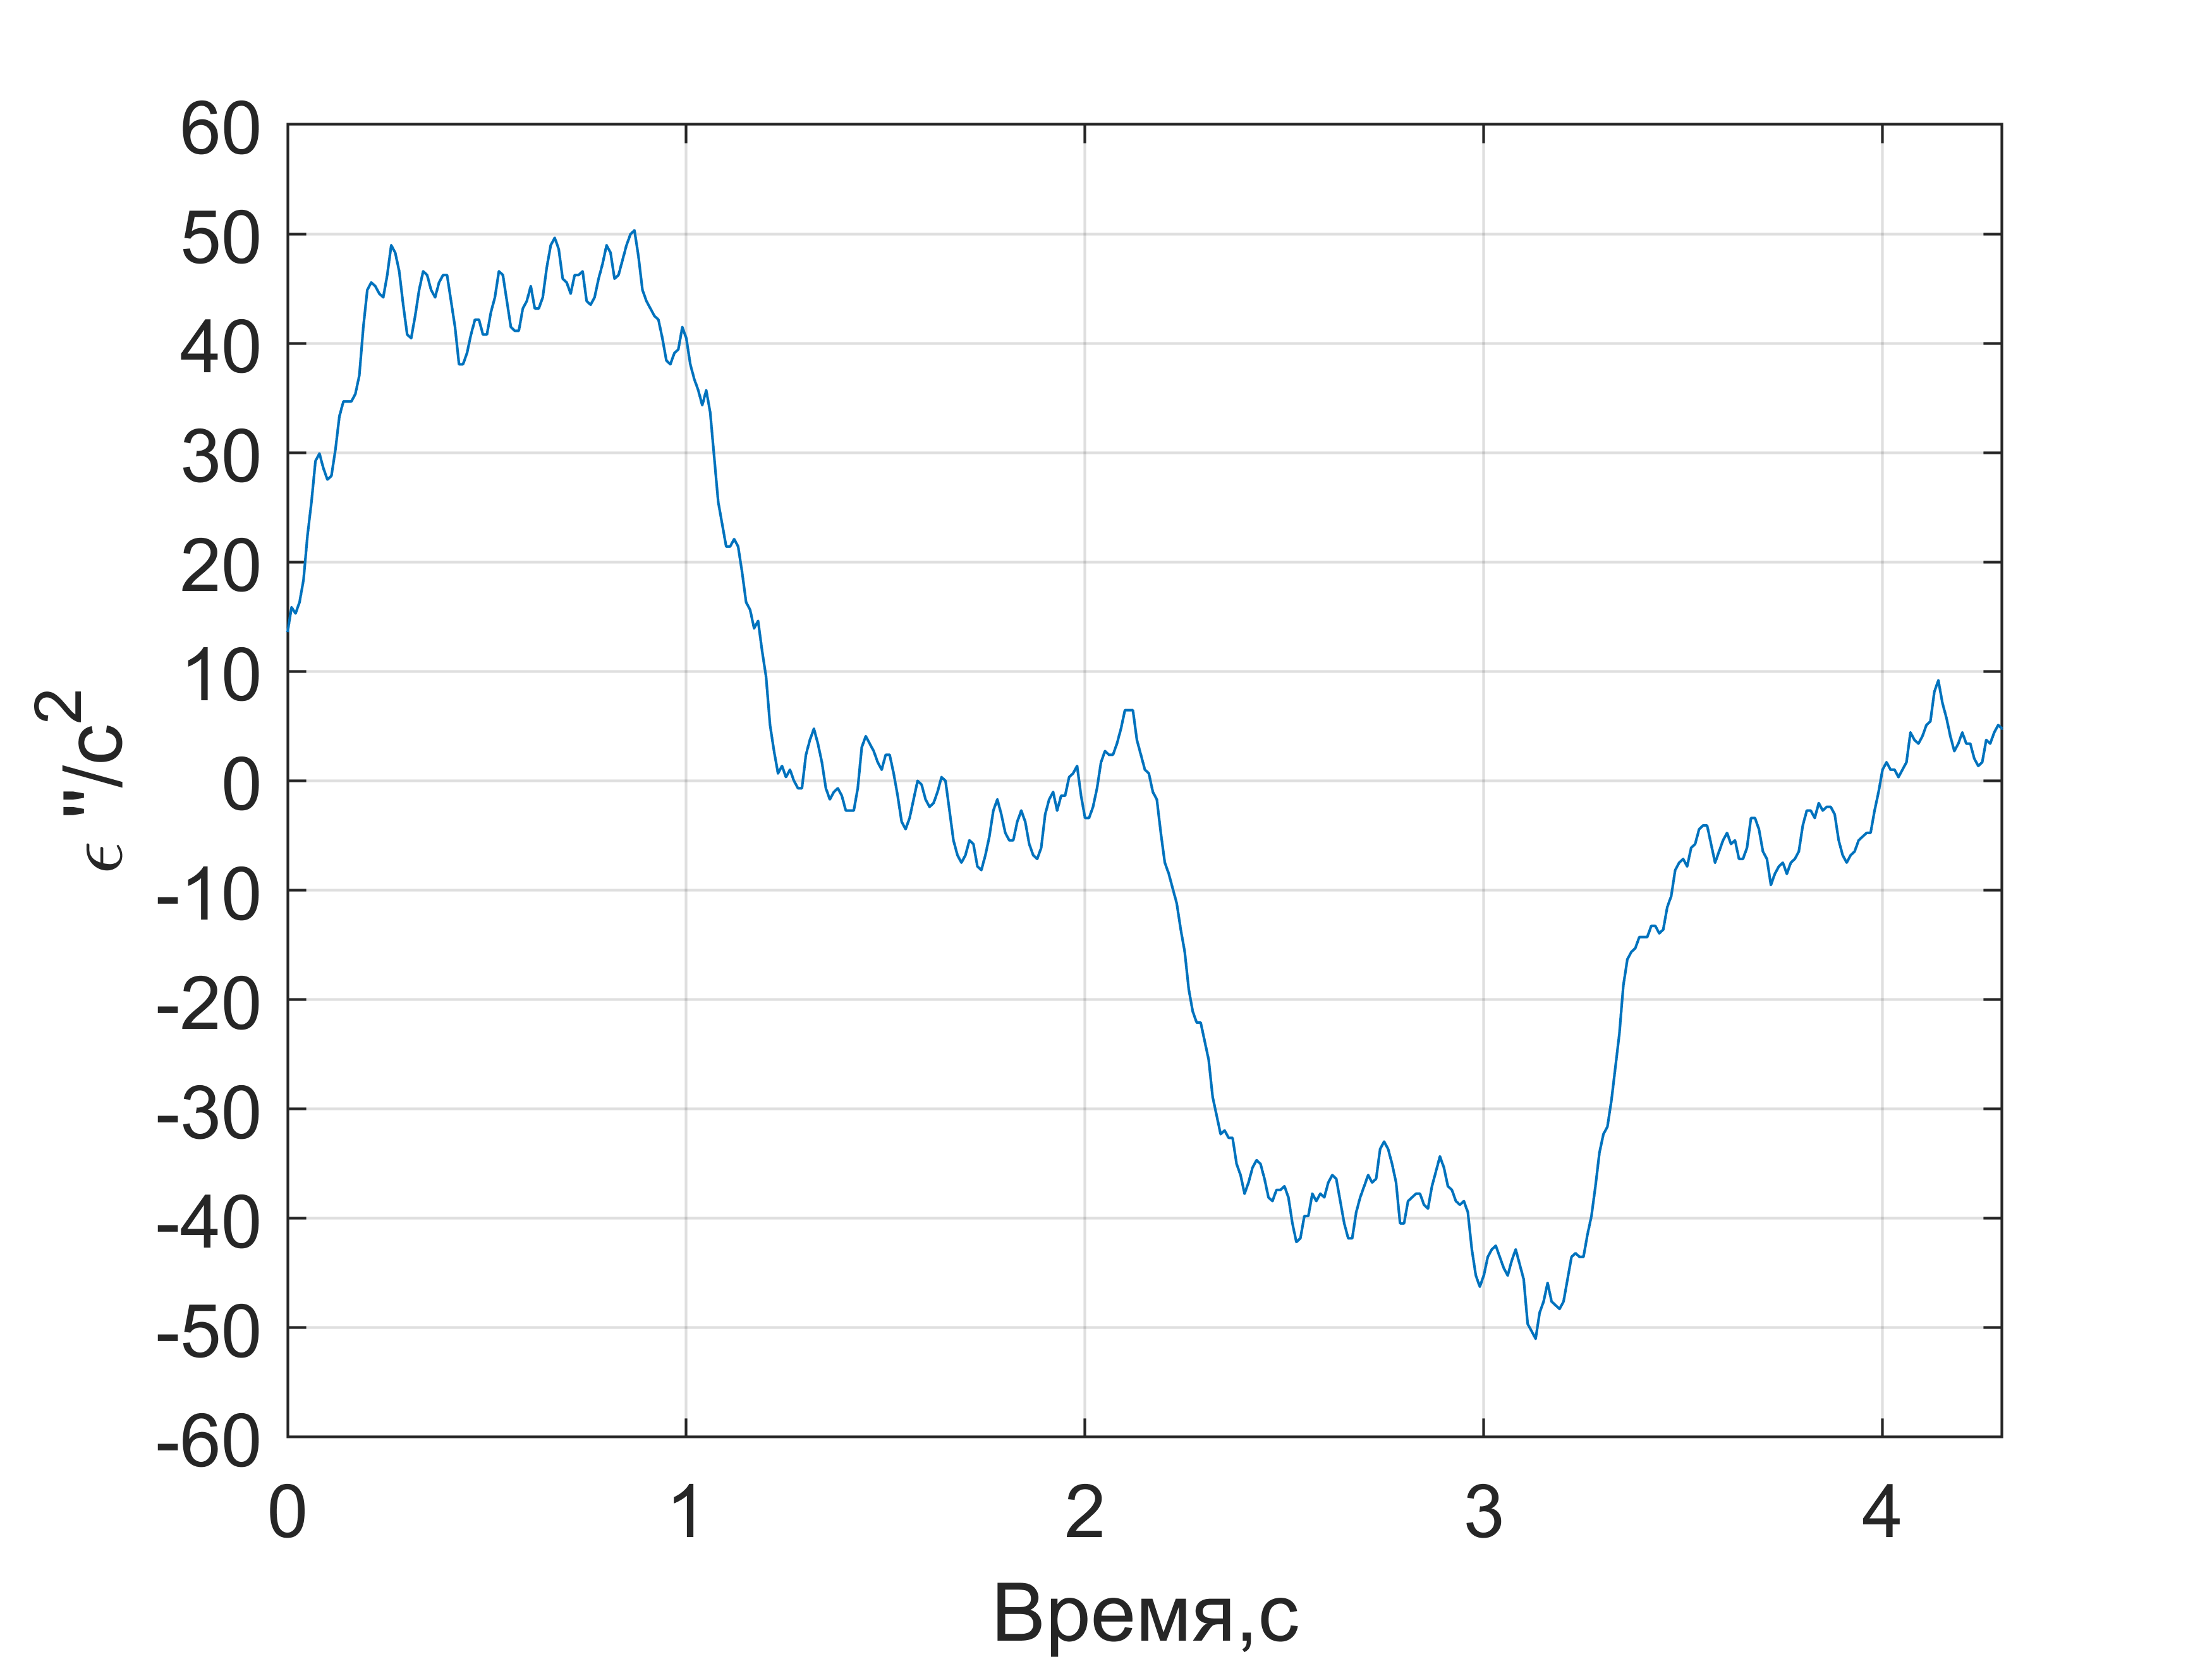
\includegraphics[scale=0.8]{matlab/img/test-gyro-acc}
	\caption{Угловое ускорение колебаний стенда при серии тестовых воздействий}
	\label{fig:test-gyro-acc}
\end{figure}

После получения углового ускорения колебаний платформы от воздействия тестового момента была проведена серия экспериментов с МНО. Для этого задавалось 10 поворотов блока зеркал на максимальный угол, в ходе которых регистрировался отклик подвеса. Как и в случае с тестовыми воздействиями, измеренные временные ряды угловой скорости были приведены к единой временной шкале, усреднены по ансамблю реализаций, а затем численно продифференцированы для получения углового ускорения. Результаты представлены на рисунке~\cref{fig:oz-gyro}.

\begin{figure}[!h]
	\begin{minipage}[b][][b]{0.49\linewidth}\centering
		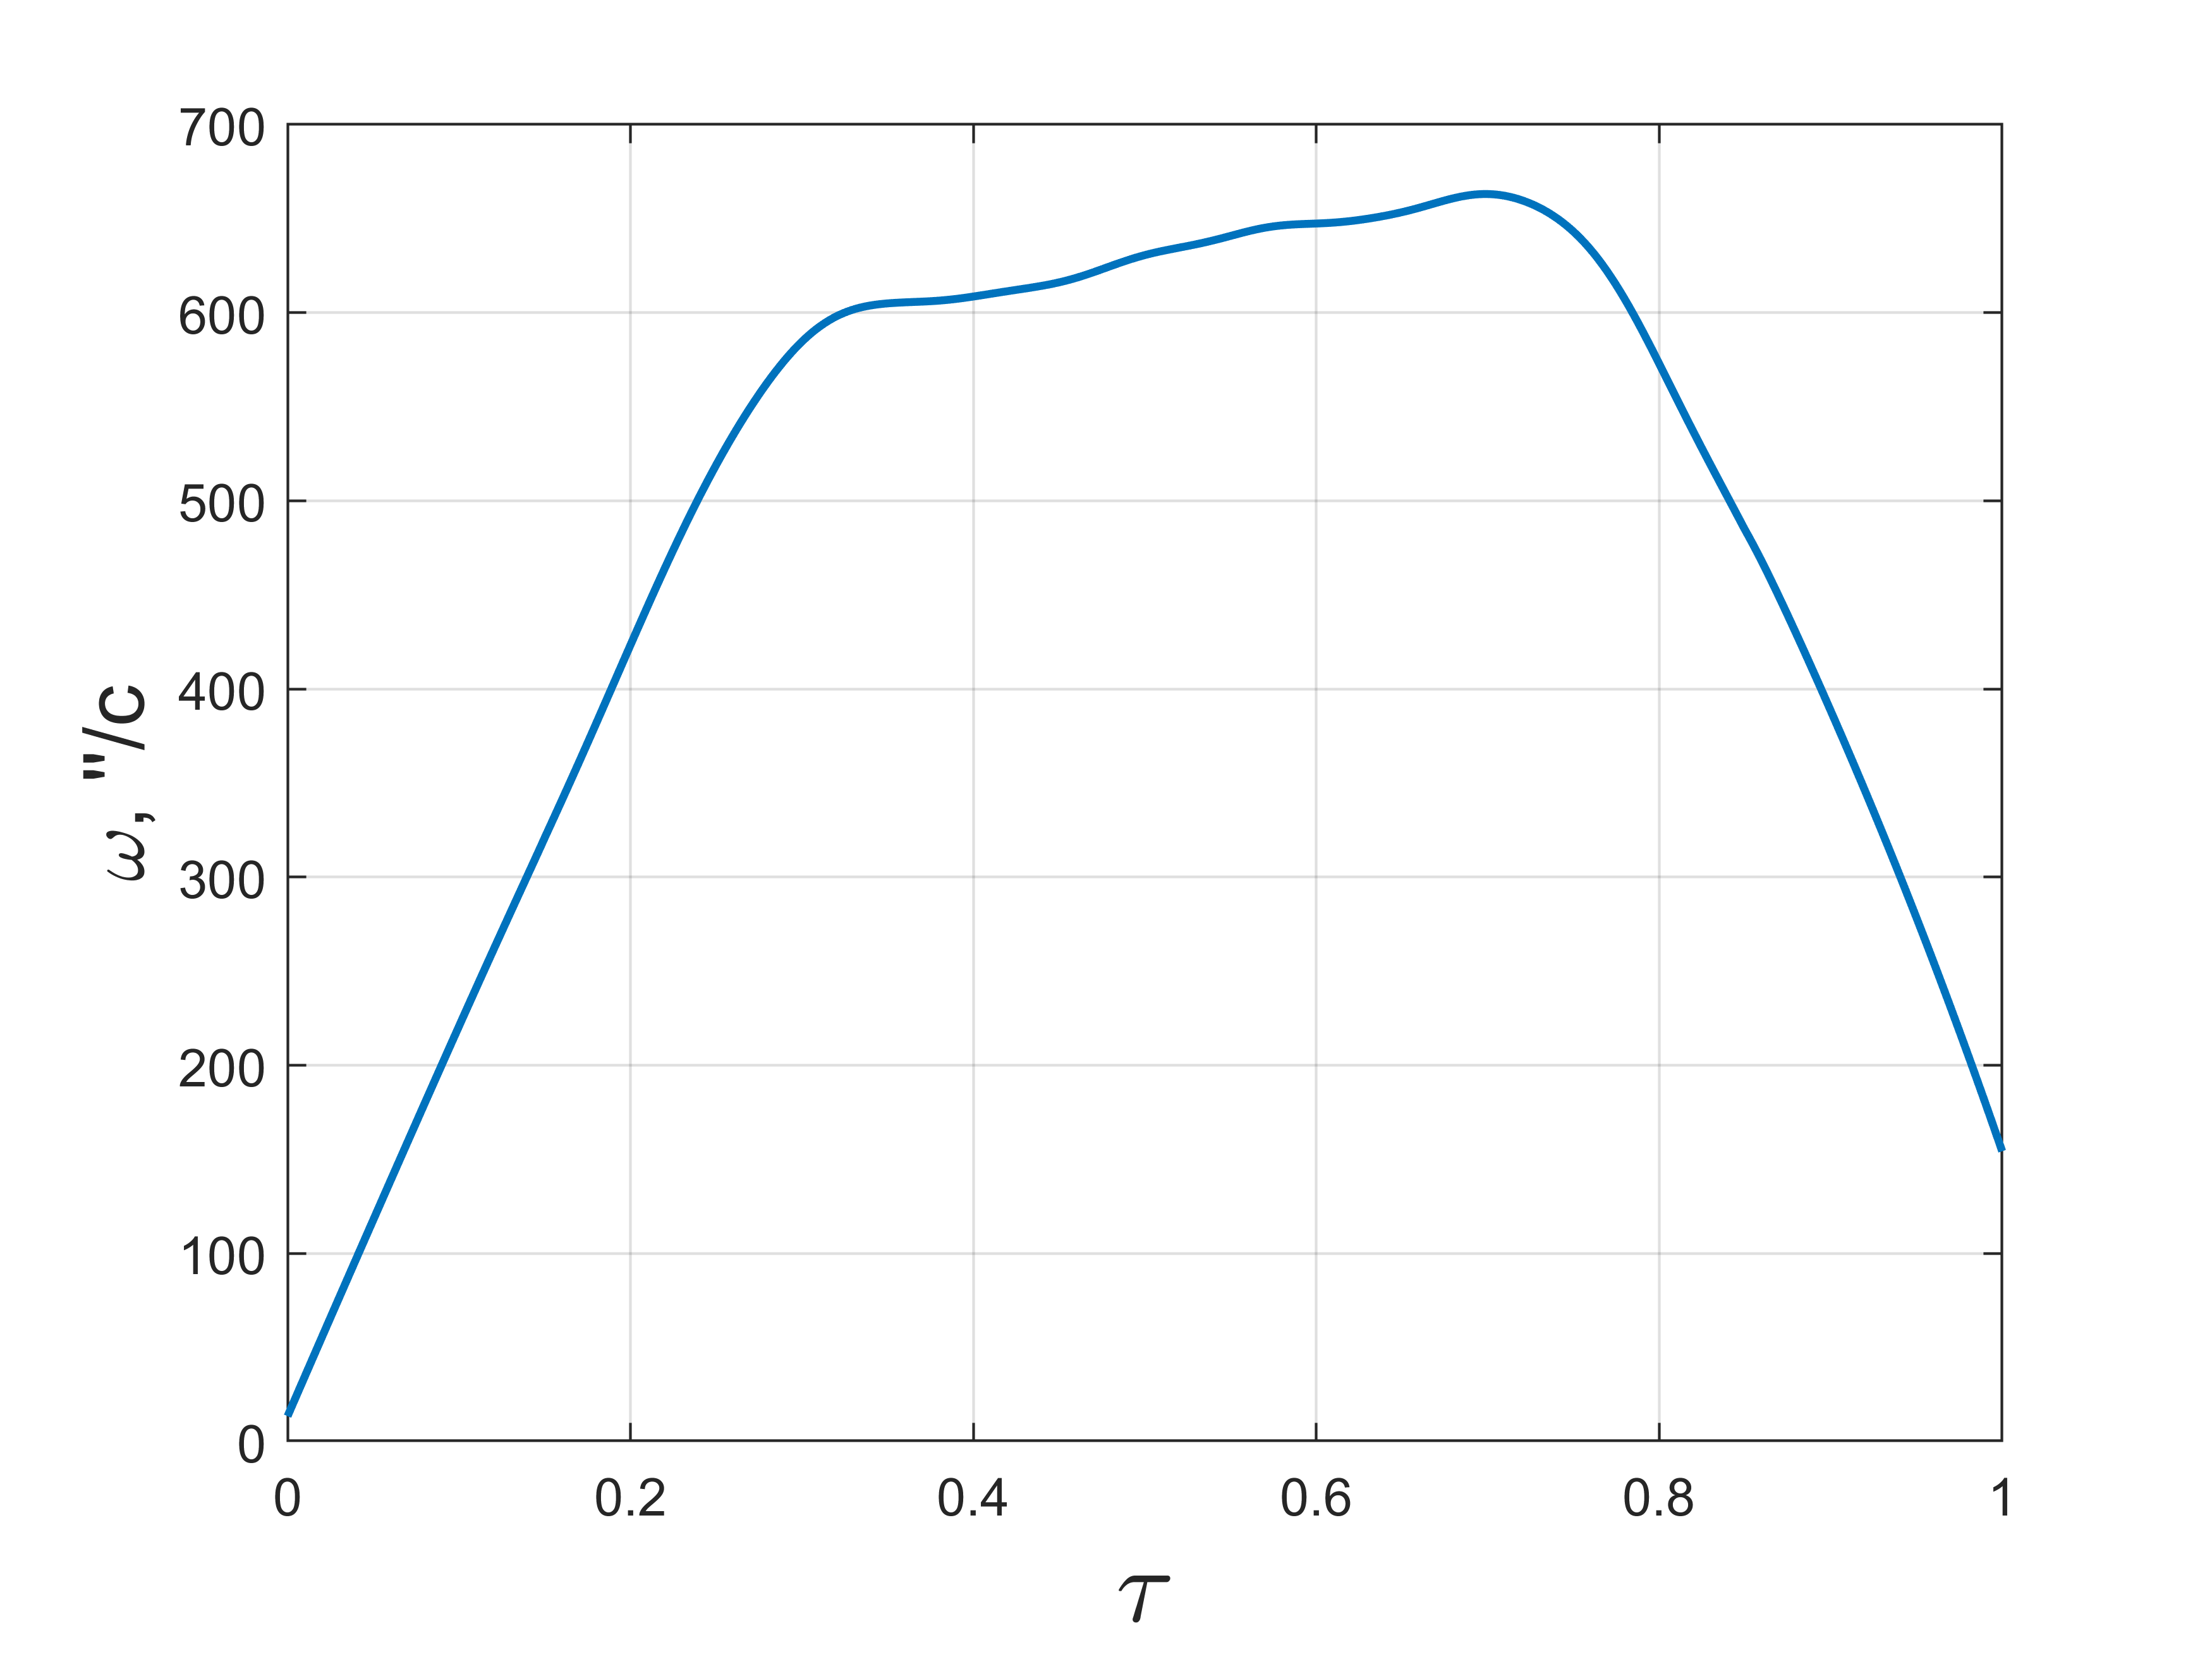
\includegraphics[width=0.9\linewidth]{matlab/img/oz-gyro.png} \\ a)
	\end{minipage}
	\hfill
	\begin{minipage}[b][][b]{0.49\linewidth}\centering
		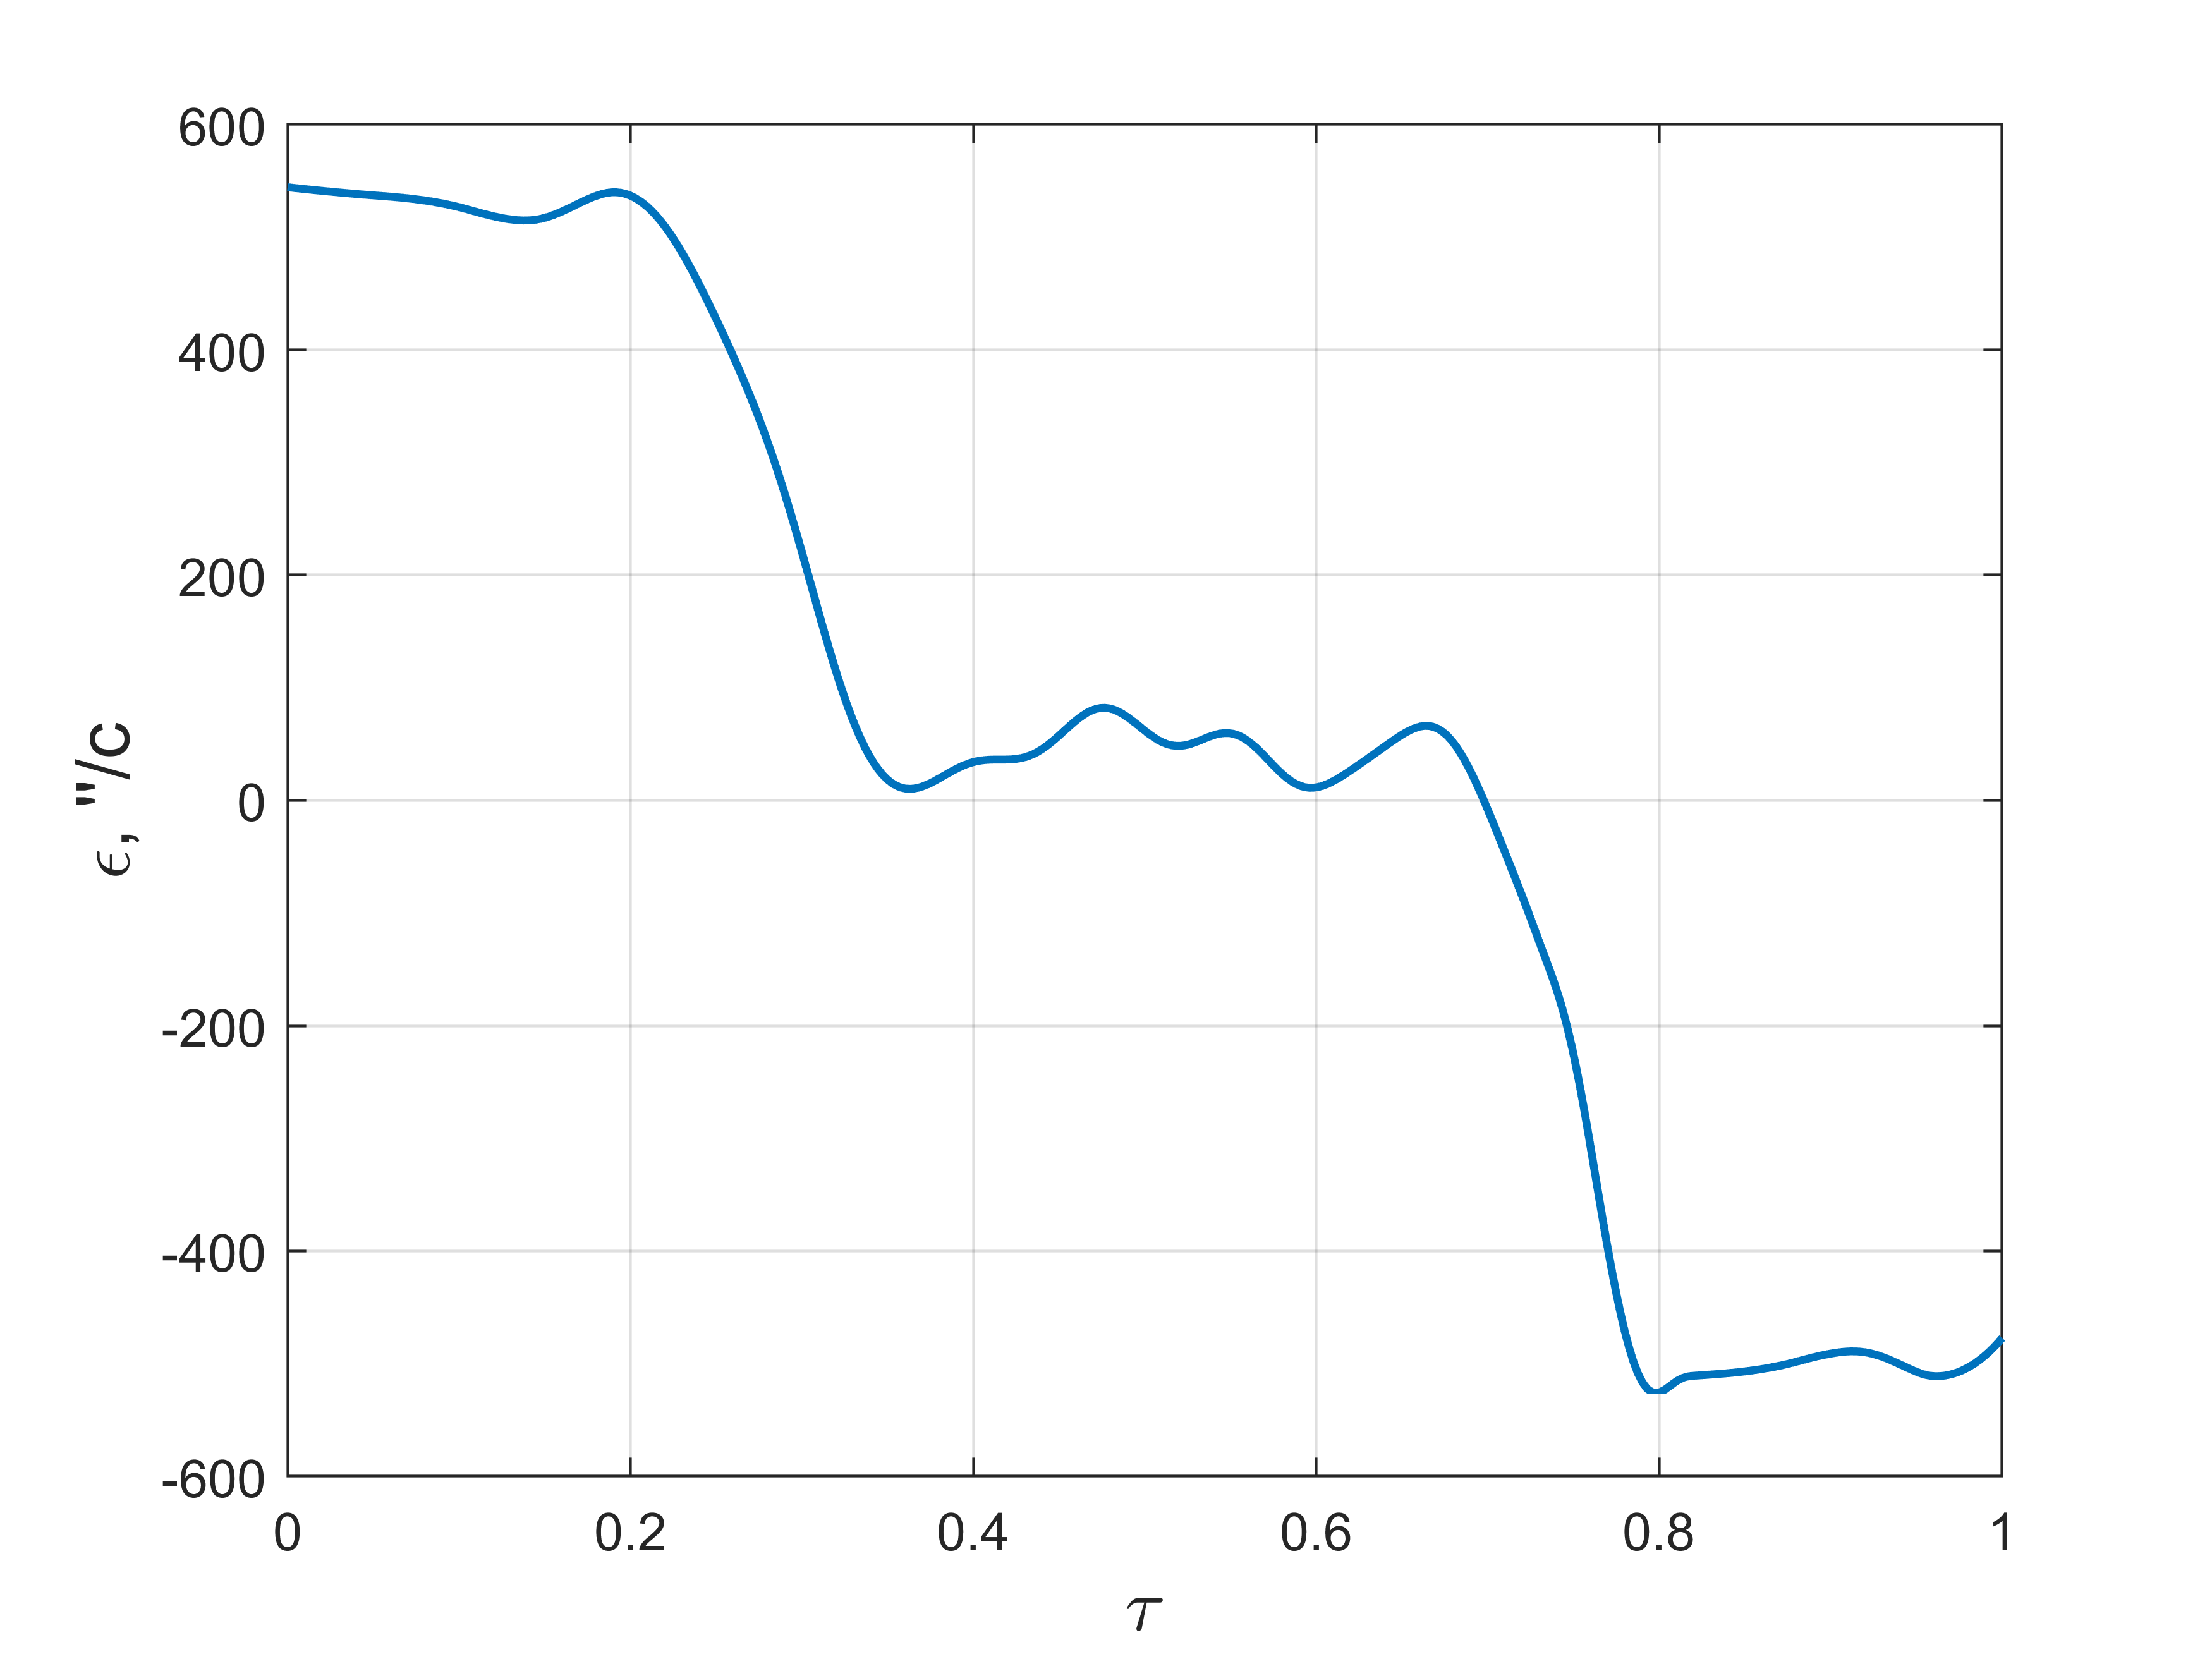
\includegraphics[width=0.9\linewidth]{matlab/img/oz-gyro-acc.png} \\ б)
	\end{minipage}
	\caption{Реакция рамы на поворот МНО вокруг оси $OZ$) скорость, б) ускорение }
	\label{fig:oz-gyro}
\end{figure}

Далее МНО была повёрнута на $\SI{90}{\degree}$ вокруг оси визирования, для оценки реактивного момента при повороте блока зеркал вокруг оси $Y$. Аналогично была по серии поворотов блока зеркал были определены скорость и ускорение колебаний рамы. Полученные результаты представлены на рисунке~\cref{fig:oy-gyro}.

\begin{figure}[!h]
	\begin{minipage}[b][][b]{0.49\linewidth}\centering
		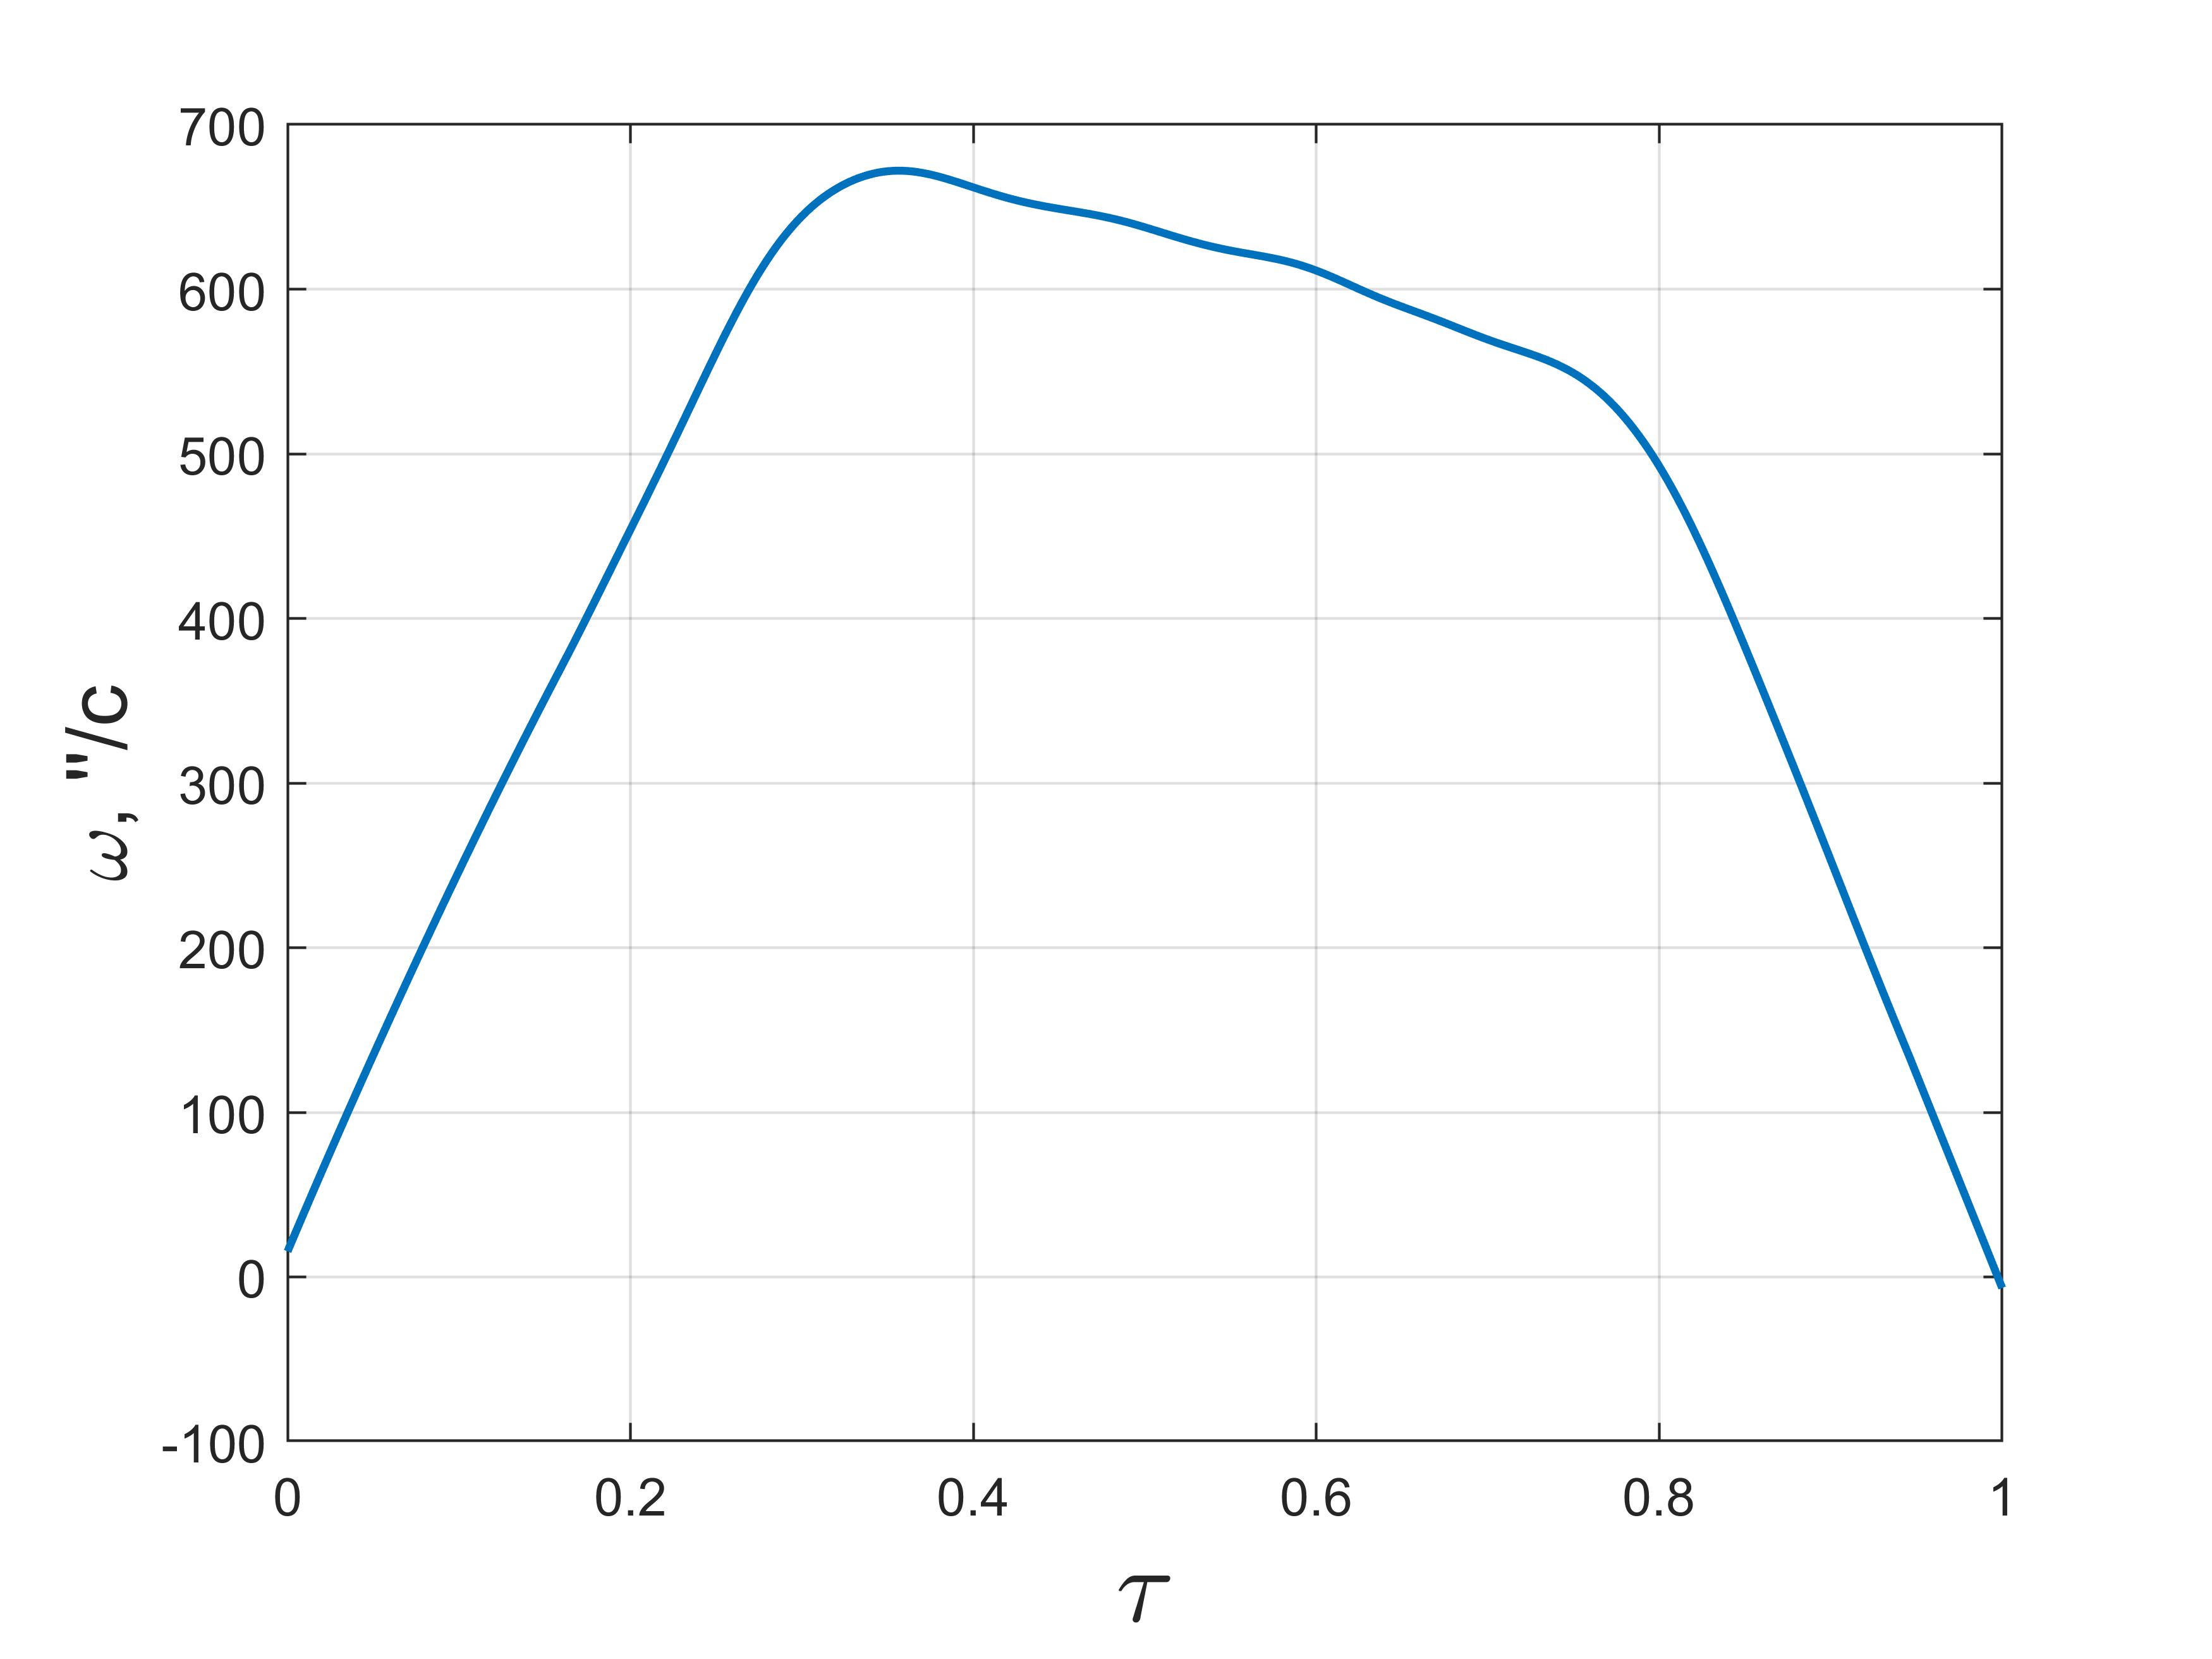
\includegraphics[width=0.9\linewidth]{matlab/img/oy-gyro.png} \\ a)
	\end{minipage}
	\hfill
	\begin{minipage}[b][][b]{0.49\linewidth}\centering
		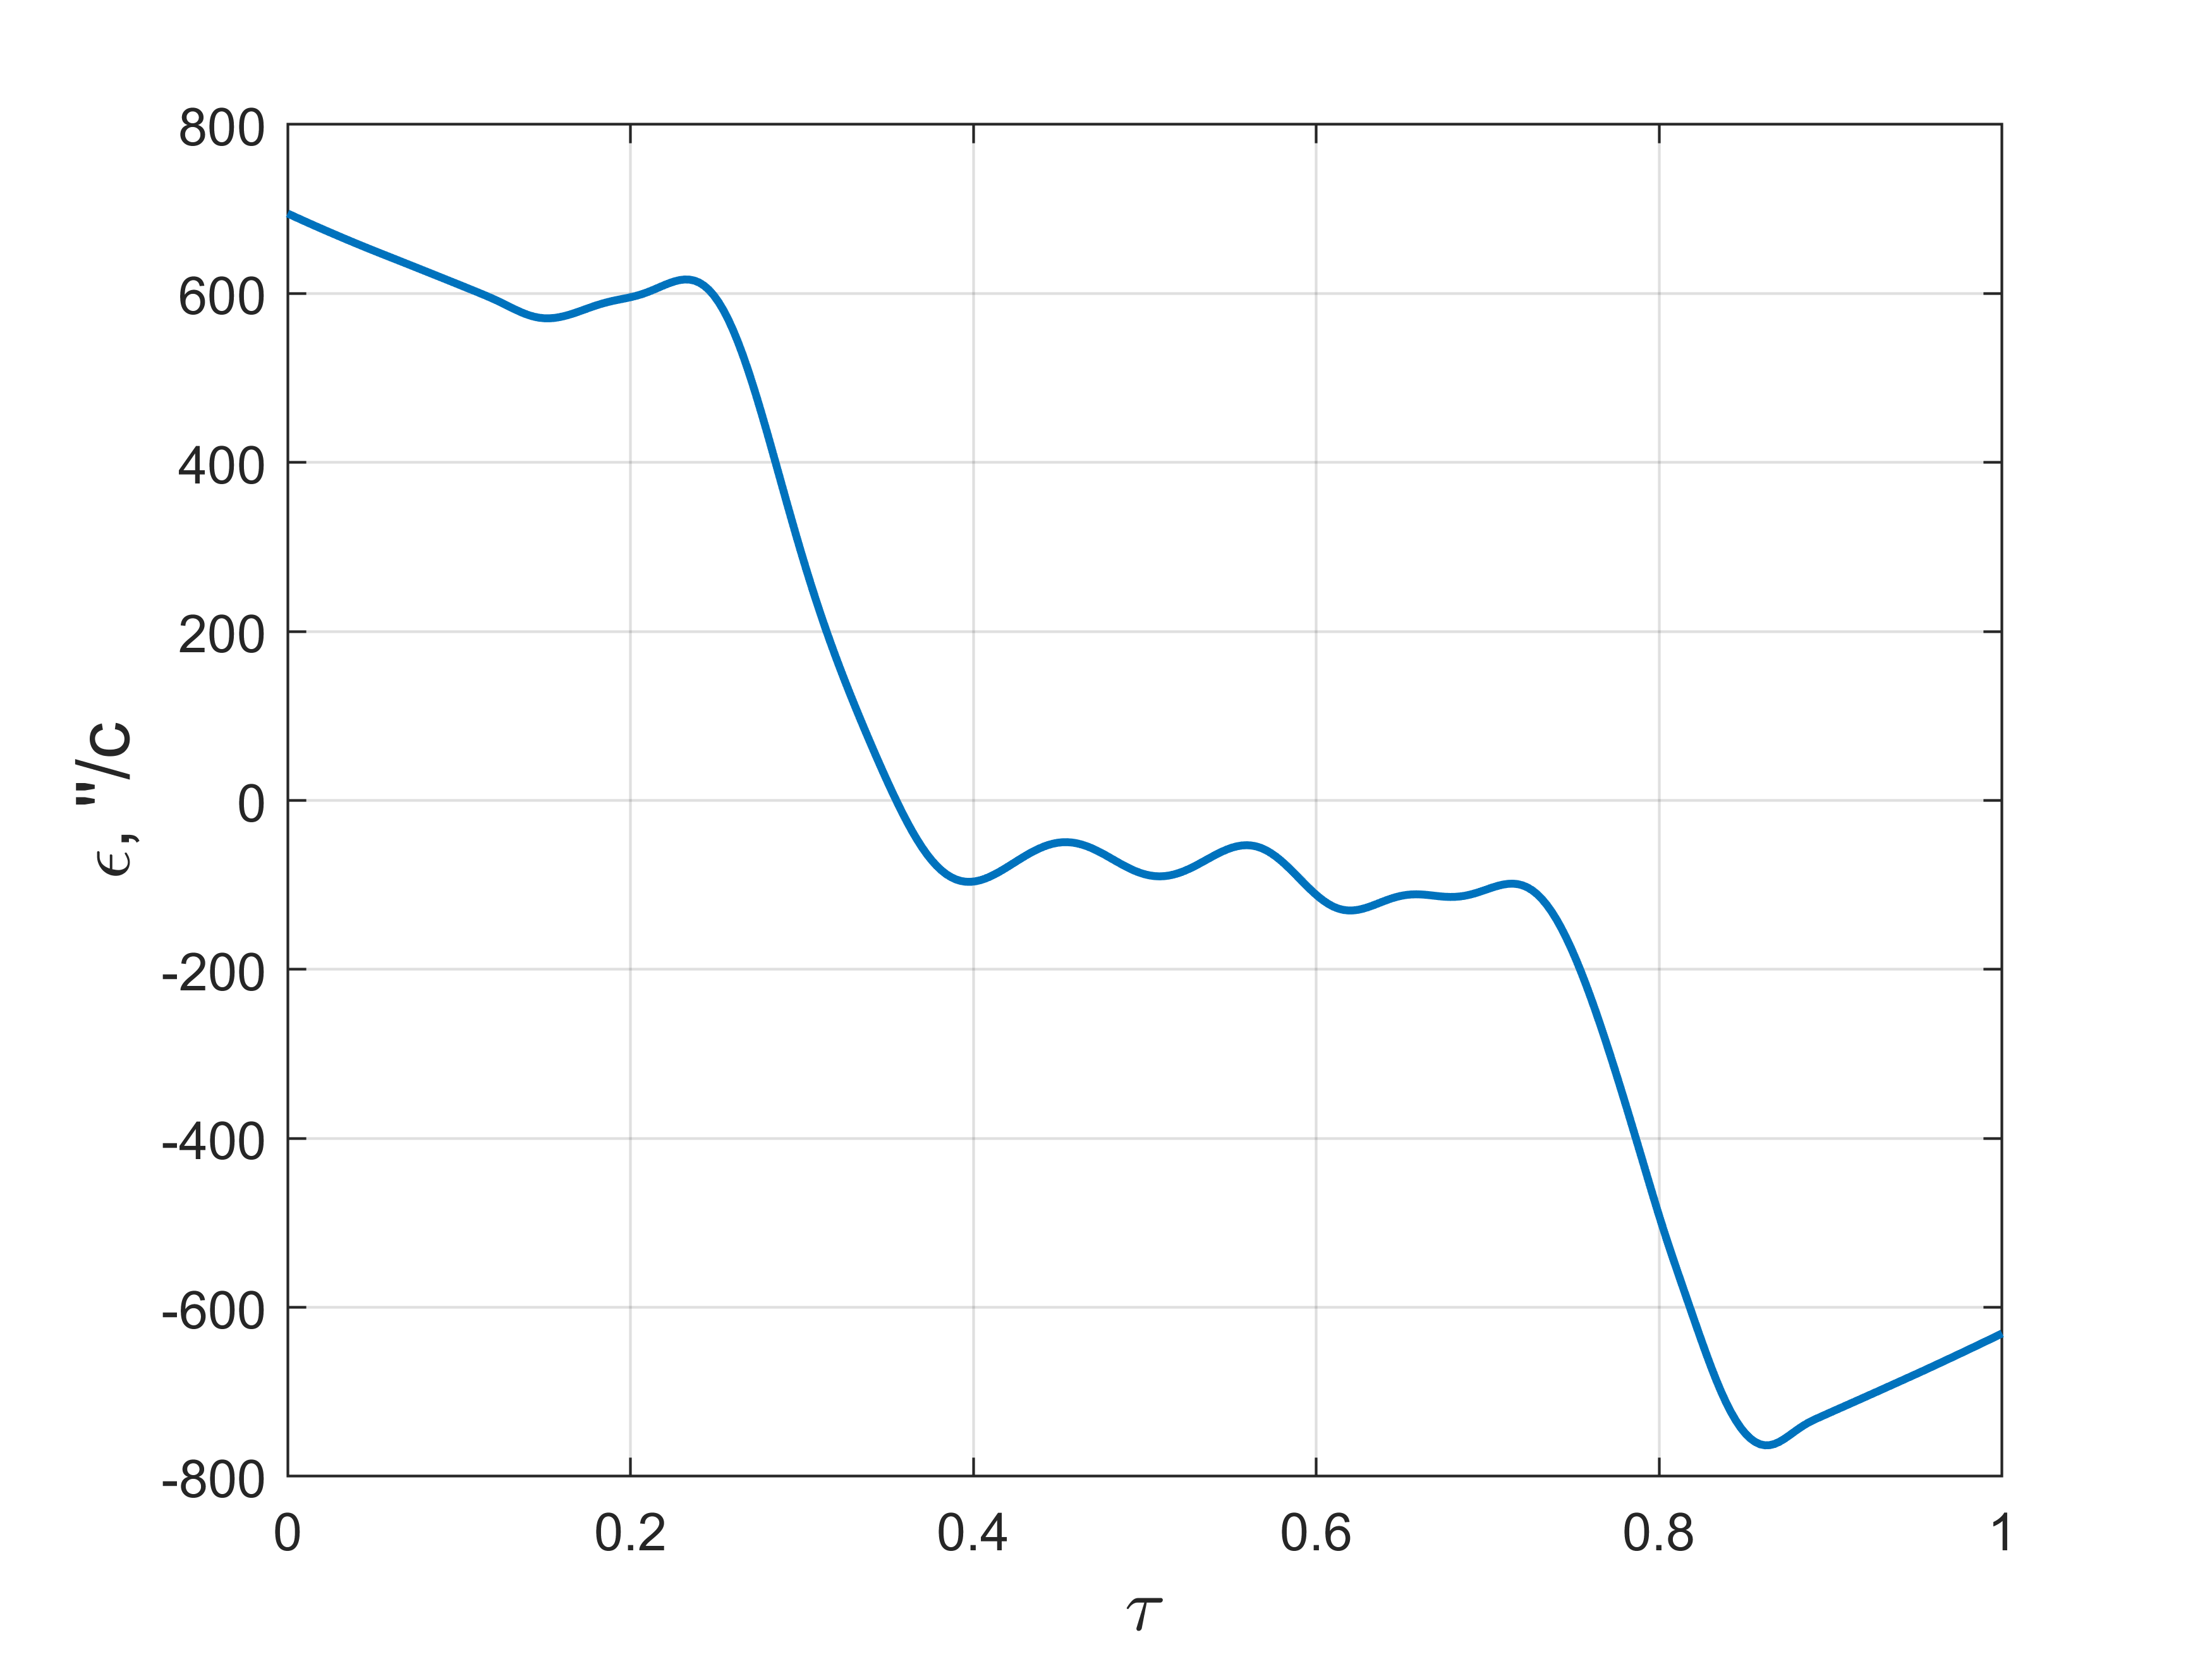
\includegraphics[width=0.9\linewidth]{matlab/img/oy-gyro-acc.png} \\ б)
	\end{minipage}
	\caption{Реакция рамы на поворот МНО вокруг оси $OY$ \\а) скорость, б) ускорение }
	\label{fig:oy-gyro}
\end{figure}


Сравнение амплитуд усреднённых ускорений, вызванных тестовым моментом и поворотом МНО, позволило определить эквивалентный момент от исследуемого узла:

\begin{equation}
	M_{\text{МНО}} = M_{\text{тест}} \cdot \frac{\varepsilon_{\text{МНО}}}{\varepsilon_{\text{тест}}}.
\end{equation}

Так как момент инерции подвесной системы $J$ во всех случаях остаётся неизменным, отношение ускорений прямо соответствует отношению действующих моментов.




\begin{figure}[!h]
	\begin{minipage}[b][][b]{0.49\linewidth}\centering
		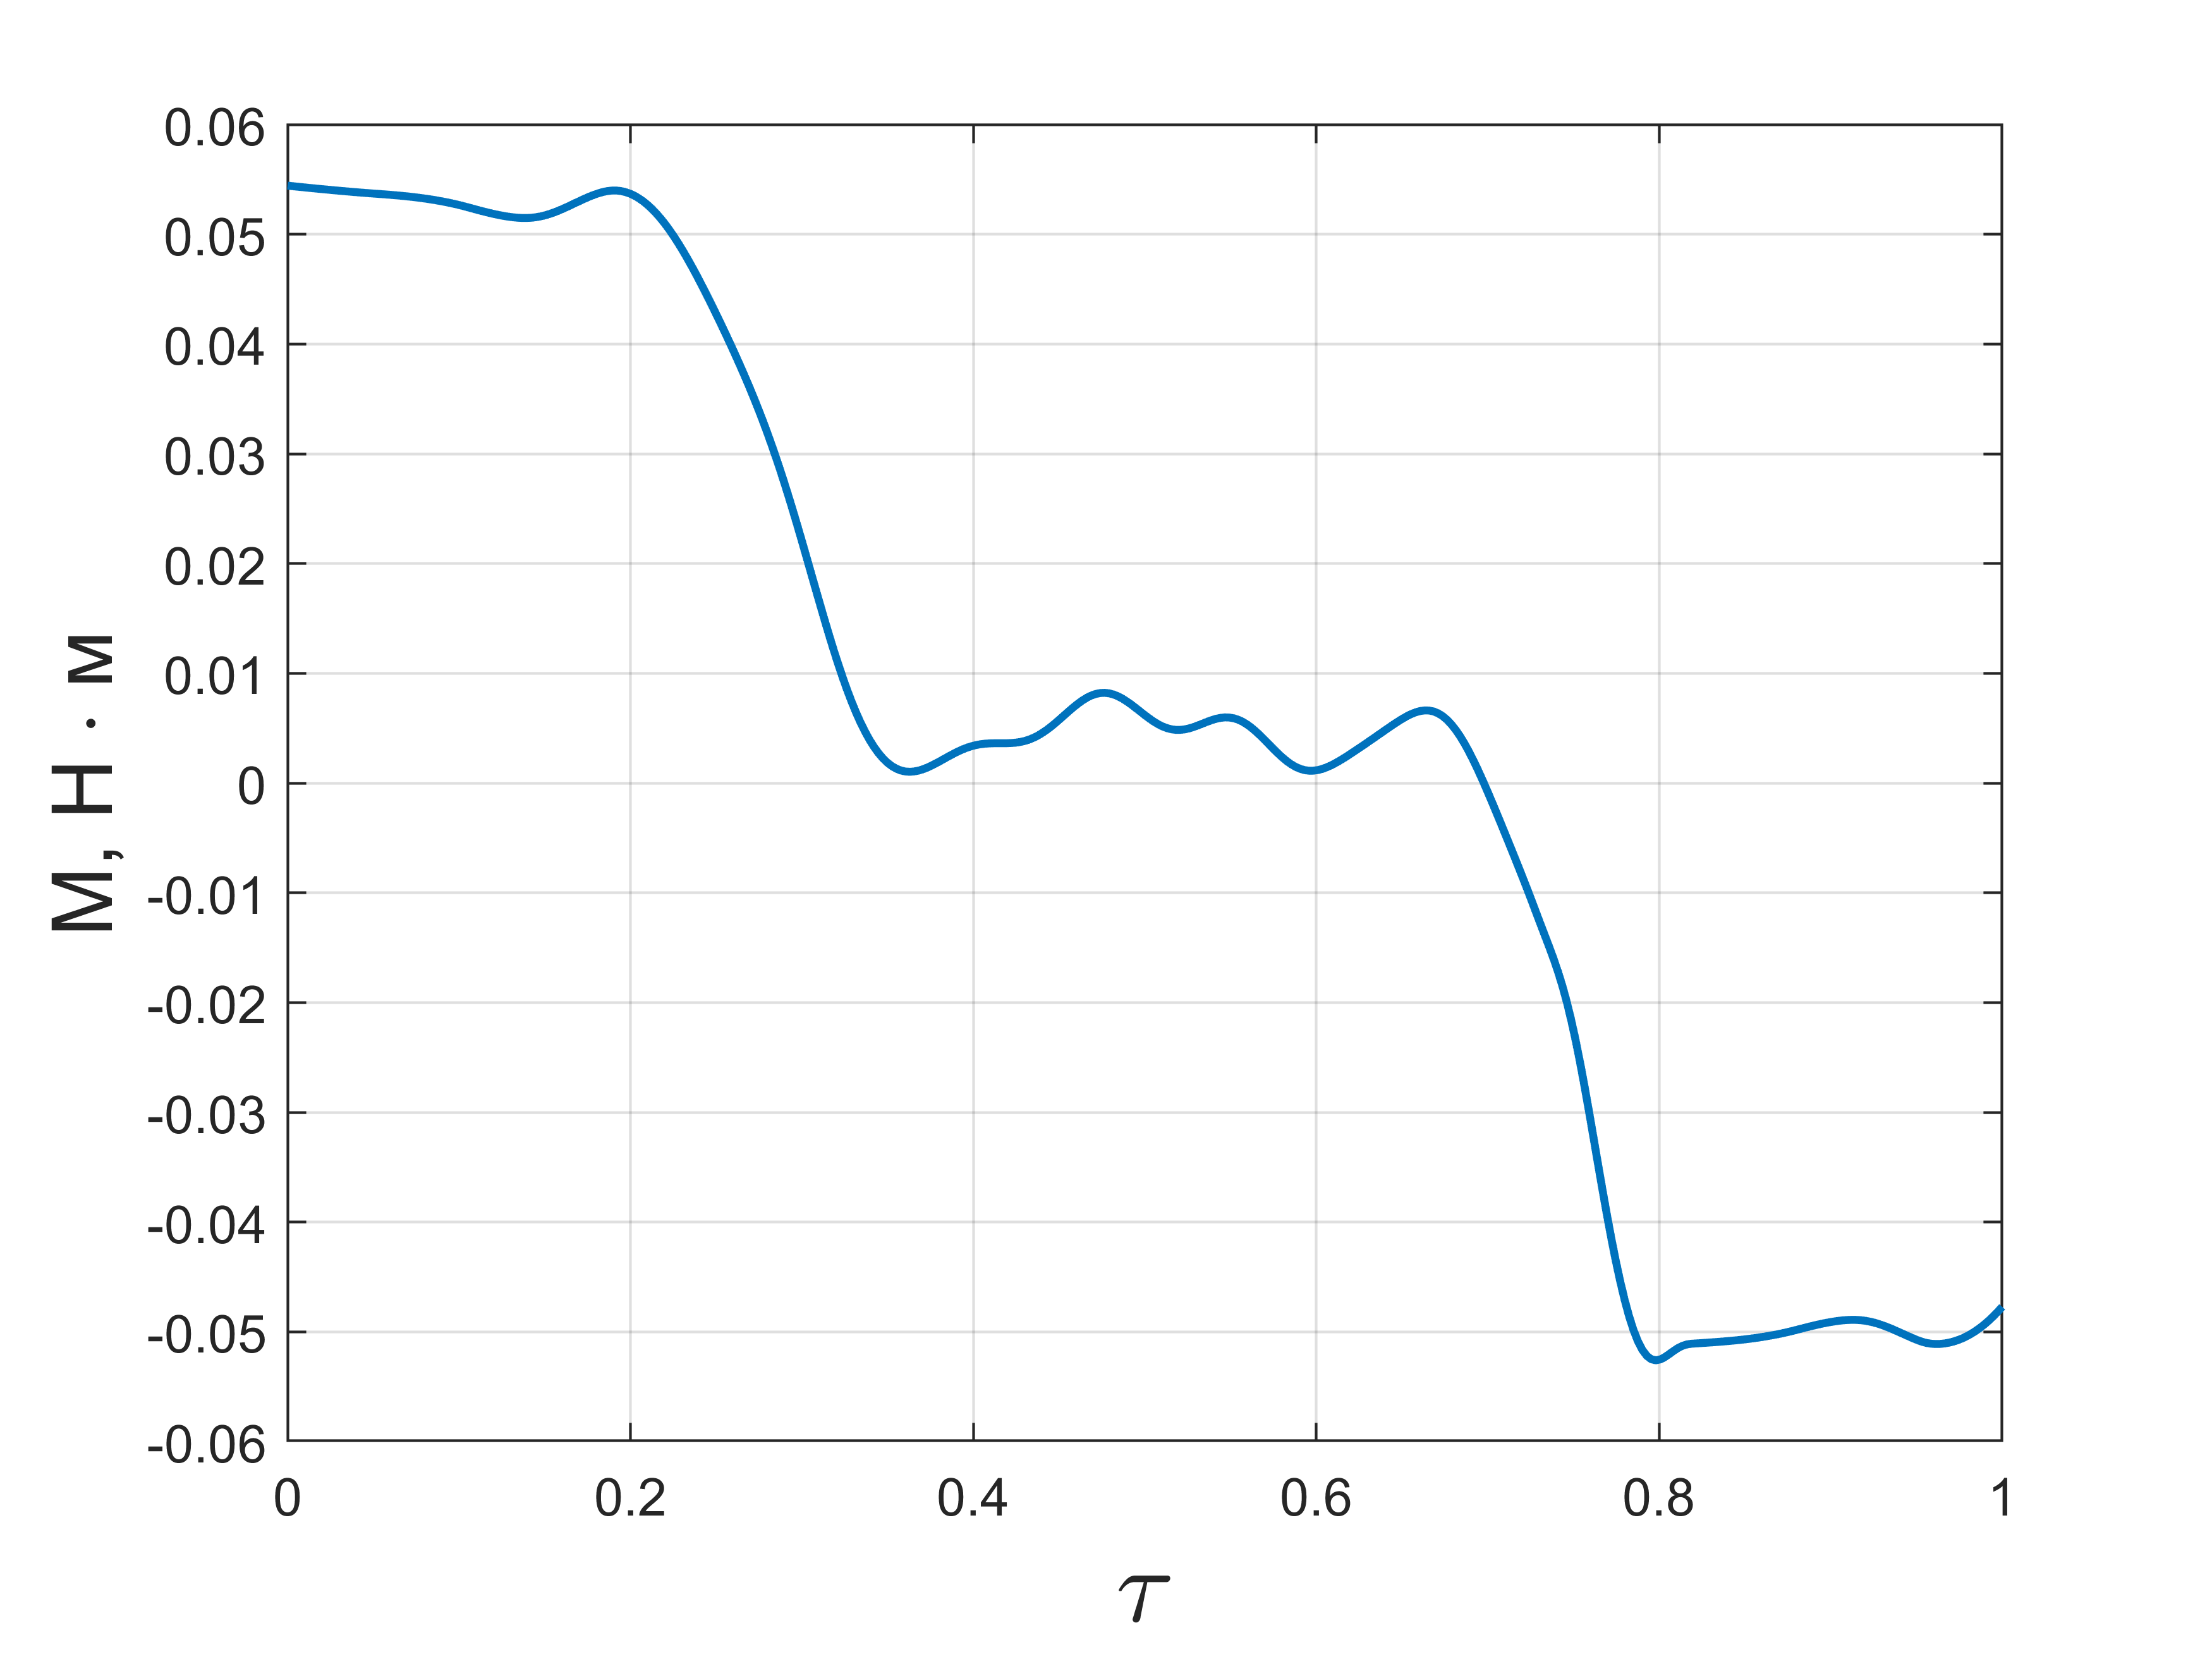
\includegraphics[width=0.9\linewidth]{matlab/img/oz-gyro-mom.png} \\ a)
	\end{minipage}
	\hfill
	\begin{minipage}[b][][b]{0.49\linewidth}\centering
		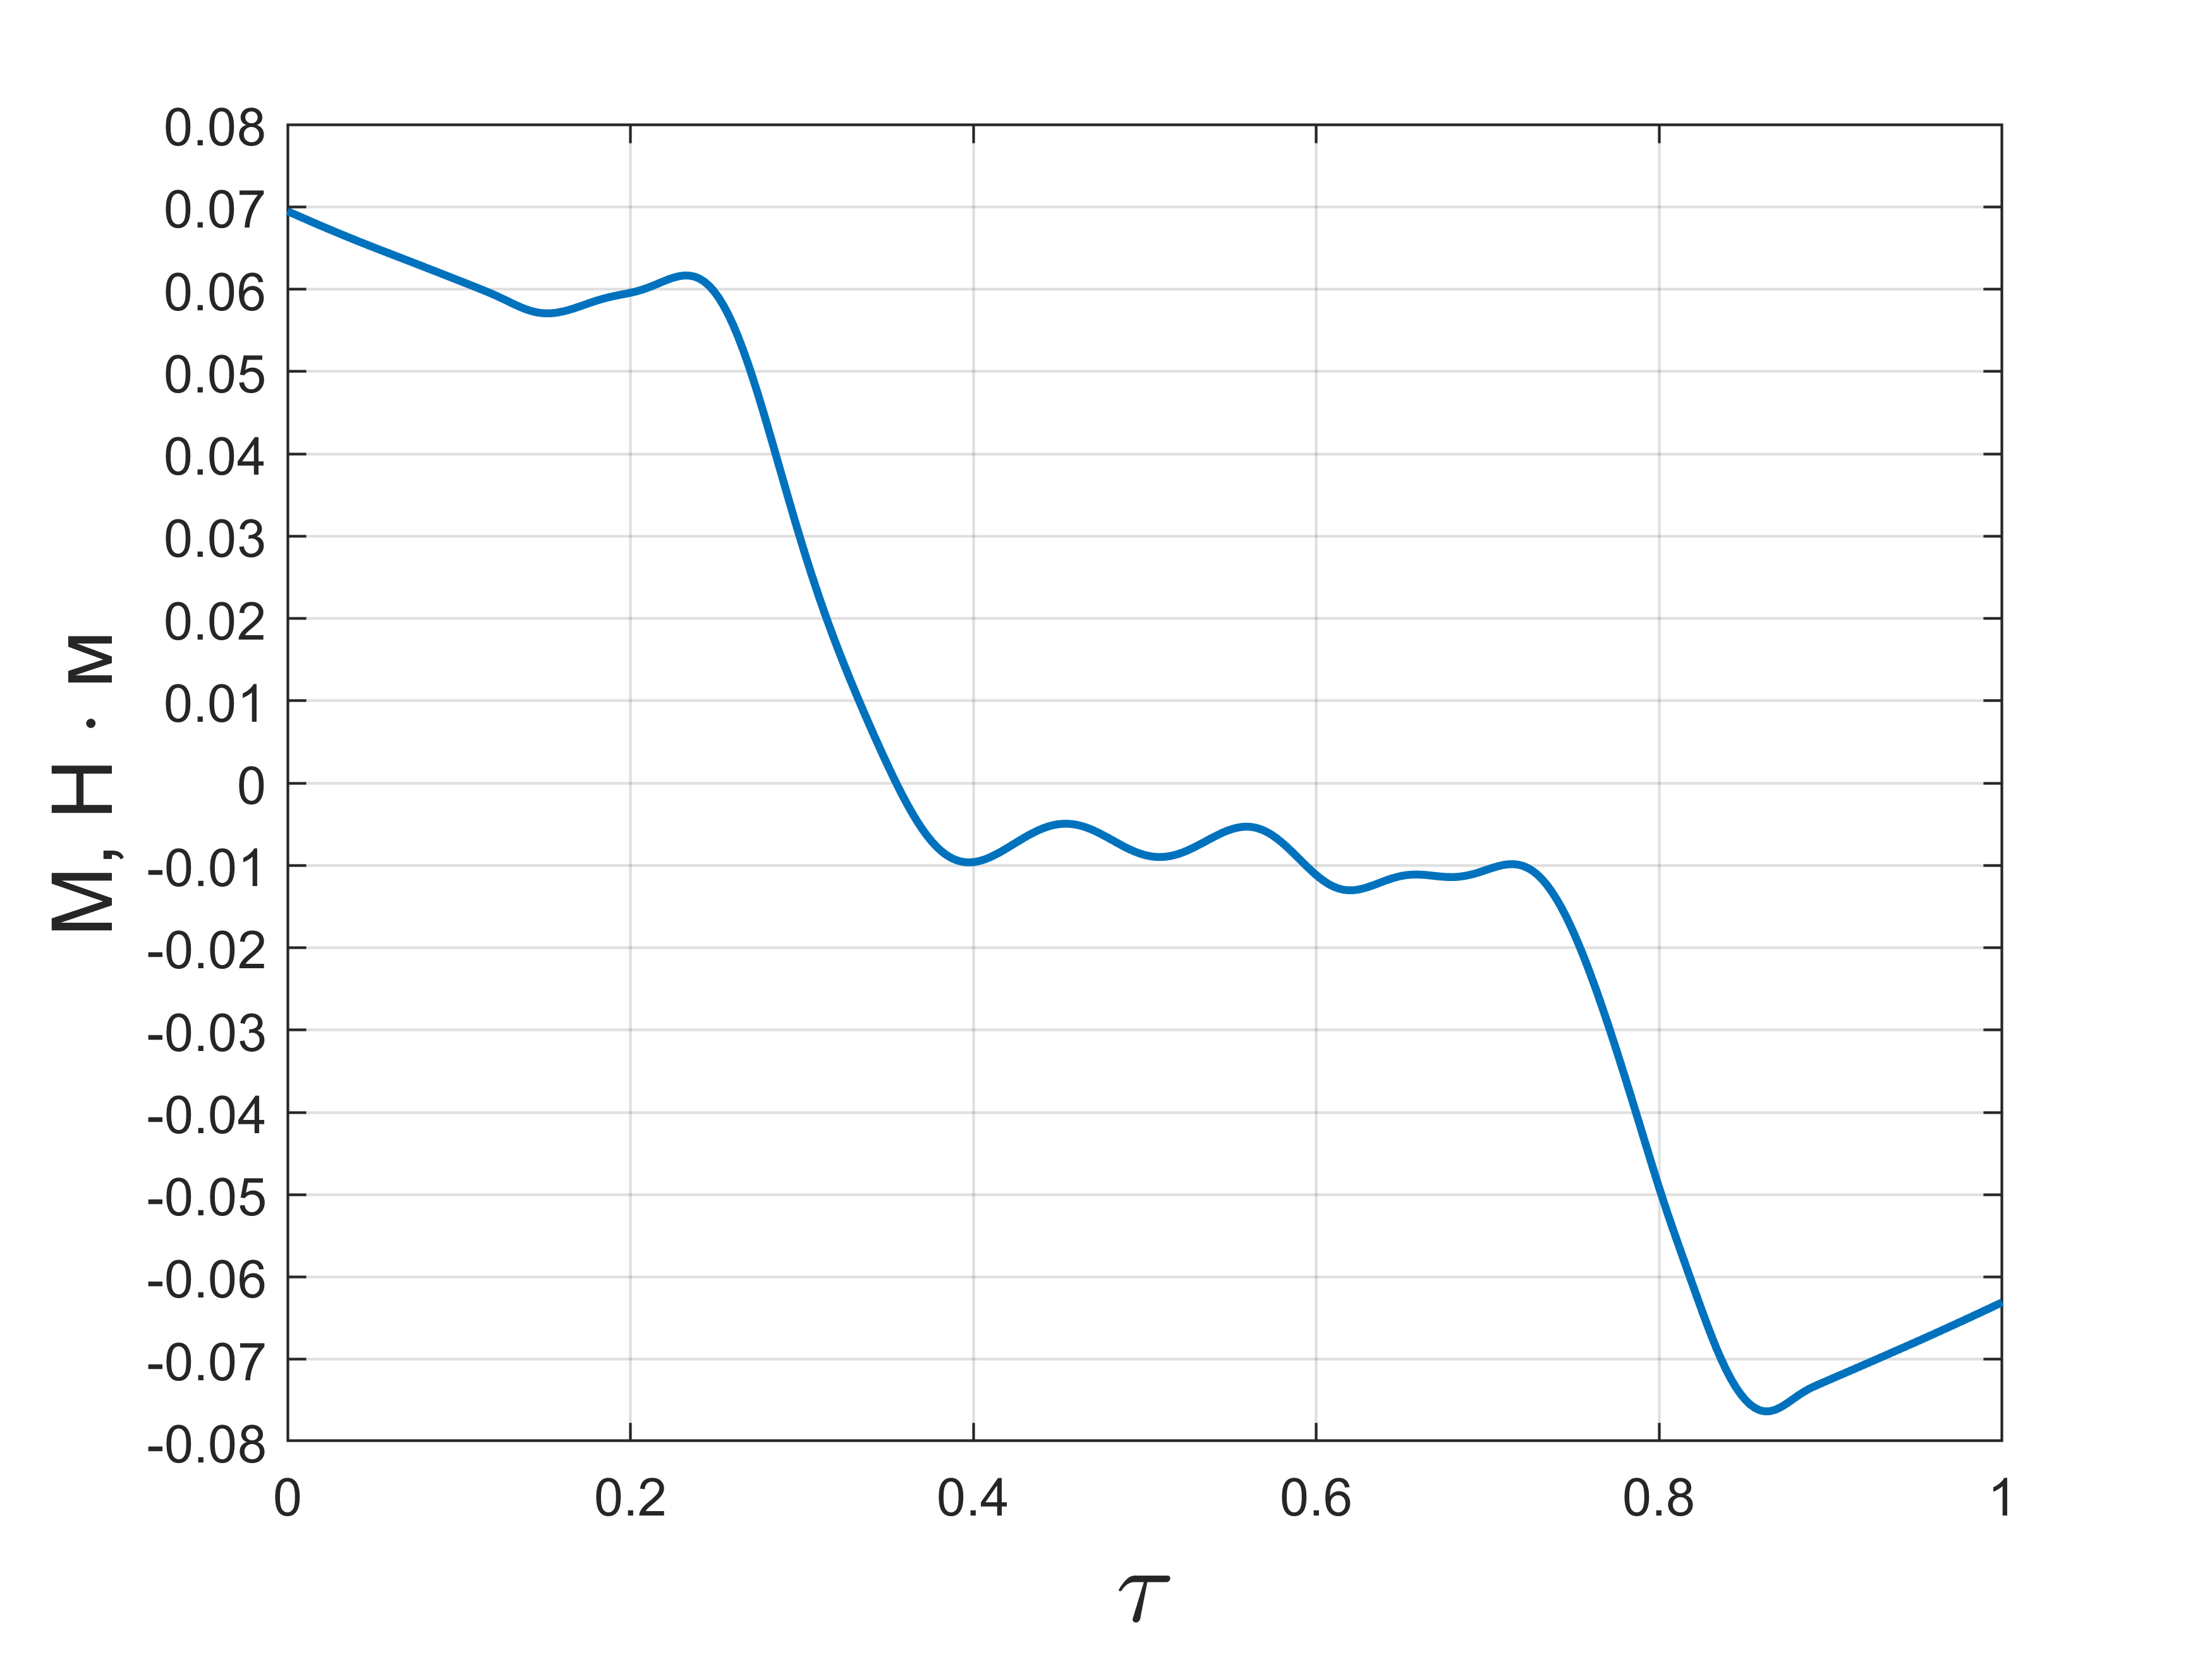
\includegraphics[width=0.9\linewidth]{matlab/img/oy-gyro-mom.png} \\ б)
	\end{minipage}
	\caption{Реакция рамы на поворот МНО вокруг оси $OY$ \\ а) скорость, б) ускорение }
	\label{fig:omn-mom}
\end{figure}

По результатам обработки экспериментальных данных величина реактивного момента составила $M_z = \SI{0,055}{\newton\meter}$ при повороте вокруг оси $Z$ и $M_y = \SI{0,076}{\newton\meter}$ при повороте вокруг оси $Y$. Полученные значения  хорошо согласуются с расчётными оценками, приведёнными во 2-й главе. Совпадение экспериментальных и теоретических данных подтверждает корректность предложенной методики измерений.
Следующим этапом работы является расчёт момента инерции дополнительных балансировочных колец, устанавливаемых на маховики устройства, с целью усиления компенсации реактивного момента.

\section{Расчёт балансировочных колец компенсирующих маховиков}



Для компенсации остаточного реактивного момента предусмотрена установка дополнительных балансировочных колец на маховики. Геометрические параметры колец заданы внешним и внутренним радиусами, а расчёту подлежит их толщина. Кольца изготавливаются из листовой латуни, при этом расчётные значения толщины заменяются ближайшими стандартными размерами листового проката. Такой подход позволяет обеспечить требуемый момент инерции маховиков и согласовать его с моментом инерции подвижной части карданного подвеса по соответствующей оси.



%todo таблица параметров маховиков

Расчёт параметров добавочных колец производился на основе сопоставления требуемого и фактического момента инерции маховика. Вначале по известным значениям момента инерции подвижной части карданова подвеса $J_y, J_z$ относительное осей $OY$ и $OZ$ и коэффициентами редукции $K_y$ и $K_z$ определялся расчётный момент инерции соответствующего маховика:

\begin{equation}
	\label{eq:inertia_flywell_calc}
	J_{my} = \frac{J_y}{K_y}, \quad \quad J_{mz}=\frac{J_z}{K_z}
	\end{equation}
	
Далее находилась величина момента инерции добавочных колец $J_{ky}$ и $J_{kz}$, которая определялась как разность между полученными расчётными и фактическими момента инерции маховиков.

По значениям наружного и внутреннего радиусов колец и рассчитанному моменту инерции определялась масса колец:

\begin{equation}
	\label{eq:flyweel_mass}
	m_{ky}=\frac{2J_{ky}}{R_{ny}^2+R_{vy}^2}, \quad \quad m_{kz}=\frac{2J_{kz}}{R_{nz}^2+R_{vz}^2}
\end{equation}

Масса, в свою очередь, позволяла вычислить объём каждого кольца с учётом плотности материала $\rho$:

\begin{equation}
	\label{eq:flyweel_volume}
	V_{ky} = \frac{m_{ky}}{\rho}, \quad V_{kz}=\frac{M_kz}{\rho}
	\end{equation}
	
	
Толщина колец определялась из соотношения объёма и площади кольцевого сечения:

\begin{equation}
	\label{eq:flywell_thickness}
	H_y=\frac{V_{ky}}{\pi(R_{ny}^2-R_{vy}^2)}, \quad H_z=\frac{V_{kz}}{\pi(R_{nz}^2-R_{vz}^2)}
	\end{equation}
Поскольку кольца изготавливались из листовой латуни, расчётные значения толщины заменялись ближайшими стандартными размерами. В случае необходимости толщина обеспечивалась набором из нескольких пластин.Для выбранной толщины $H_{y_{0}}, H_{z_{0}}$ пересчитывались моменты инерции колец, для уточнения соответствия рассчётным значениям:

\begin{equation}
	\label{eq:final_ring_inertia}
	J_{ky0}=J_{ky}\frac{H_y}{H_{y_{0}}}, \quad J_{kz_{0}}=J_{kz}\frac{H_z}{H_{z_{0}}}
	\end{equation}
	
После подбора размеров выполнялся расчёт суммарного момента инерции маховиков:

\begin{equation}
	\label{eq:flyweel_sum_inertia}
	J_{y0}=J_y+J_{ky_{0}}, \quad J_{z0}=J_{z}+J_{kz_{0}}
\end{equation}

Результат расчёта параметров дополнительных колец приведён в таблице~\cref{tab:flyweel-ring}.

\sisetup{
	output-decimal-marker = {,},
	group-separator = \,,
}


\begin{table}[ht]
	\centering
	\caption{Параметры маховиков}
	\label{tab:flyweel-ring}
	
	% компактнее: меньше горизонтальных отступов и чуть плотнее строки
	\setlength{\tabcolsep}{4pt}
	\renewcommand{\arraystretch}{1.05}
	
	% масштабируем, если ширина больше \textwidth
	\resizebox{\textwidth}{!}{%
		\begin{tabular}{
				l
				S[table-format=3.0]
				S[table-format=1.4]
				S[table-format=1.4]
				S[table-format=1.4]
				S[table-format=1.4]
				S[table-format=1.4]
			}
			\toprule
			{Параметр} &
			{Коэфф.\ редукции} &
			{\makecell{Момент инерции\\подвижной части,\\кг·м$^2$}} &
			{\makecell{Расчётный момент\\инерции маховика,\\кг·м$^2$}} &
			{\makecell{Добавочный момент\\инерции,\\кг·м$^2$}} &
			{\makecell{Радиус\\наружный кольца,\\м}} &
			{\makecell{Радиус\\внутренний кольца,\\м}} \\
			\midrule
			Маховик по Y & 160 & 2,5600 & 0,0159 & 0,0015 & 0,0955 & 0,0725 \\
			Маховик по Z & 160 & 1,9000 & 0,0119 & 0,0011 & 0,1050 & 0,0900 \\
			\bottomrule
		\end{tabular}%
	}
\end{table}




\section{Повторные стендовые испытания с применением синусоидального профиля}


После расчёта и установки балансировочных колец на маховики МНО, увеличивших их момент инерции, была проведена серия повторных стендовых испытаний. Целью экспериментов являлась оценка эффективности компенсации реактивного момента в доработанной конструкции и проверка влияния нового закона управления приводом.

В отличие от первой серии, где повороты выполнялись по закону с постоянным угловым ускорение, на данном этапе использовался синусоидальный профиль управления приводом.

Методика обработки данных оставалась прежней: измеренные гироскопом временные ряды угловой скорости приводились к единой временной шкале, усреднялись по ансамблю реализаций и дифференцировались для получения углового ускорения.

На рисунке~\cref{fig:sin-profile-omn} представлены результаты измерений после установки балансировочных колец и применения синусоидального профиля: угловая скорость, угловое ускорение и эквивалентный реактивный момент по осям $OZ$ и $OY$.

\begin{figure}[h!]
	% --- Первая строка ---
	\begin{minipage}[b]{0.49\linewidth}\centering
		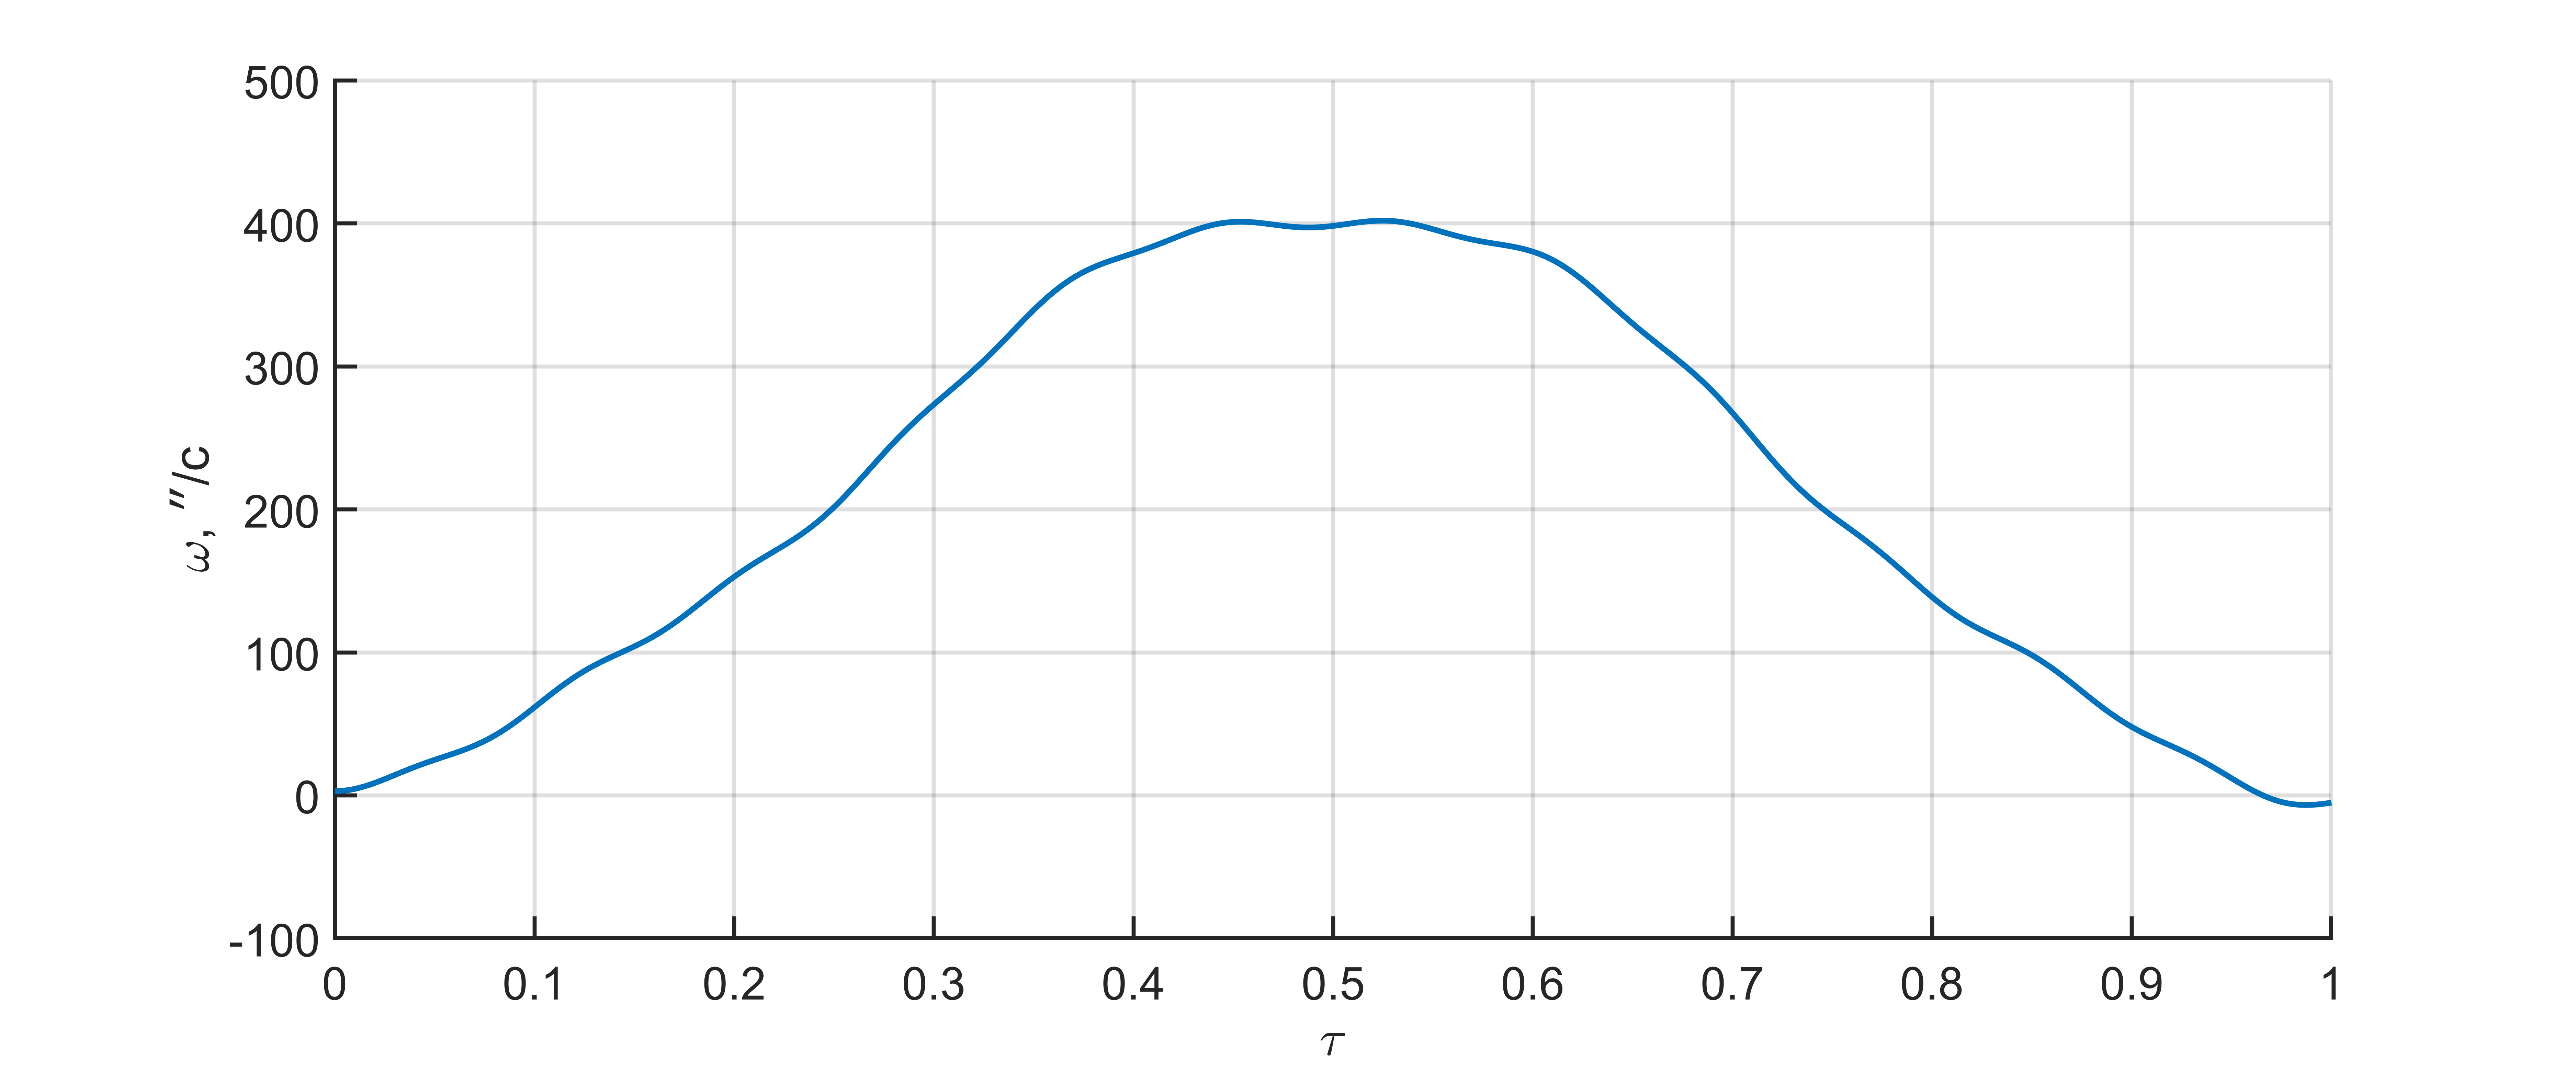
\includegraphics[width=\linewidth]{matlab/img/oz-gyro-sin-vel} \\ а) угловая скорость (ось $OZ$)
	\end{minipage}
	\hfill
	\begin{minipage}[b]{0.49\linewidth}\centering
		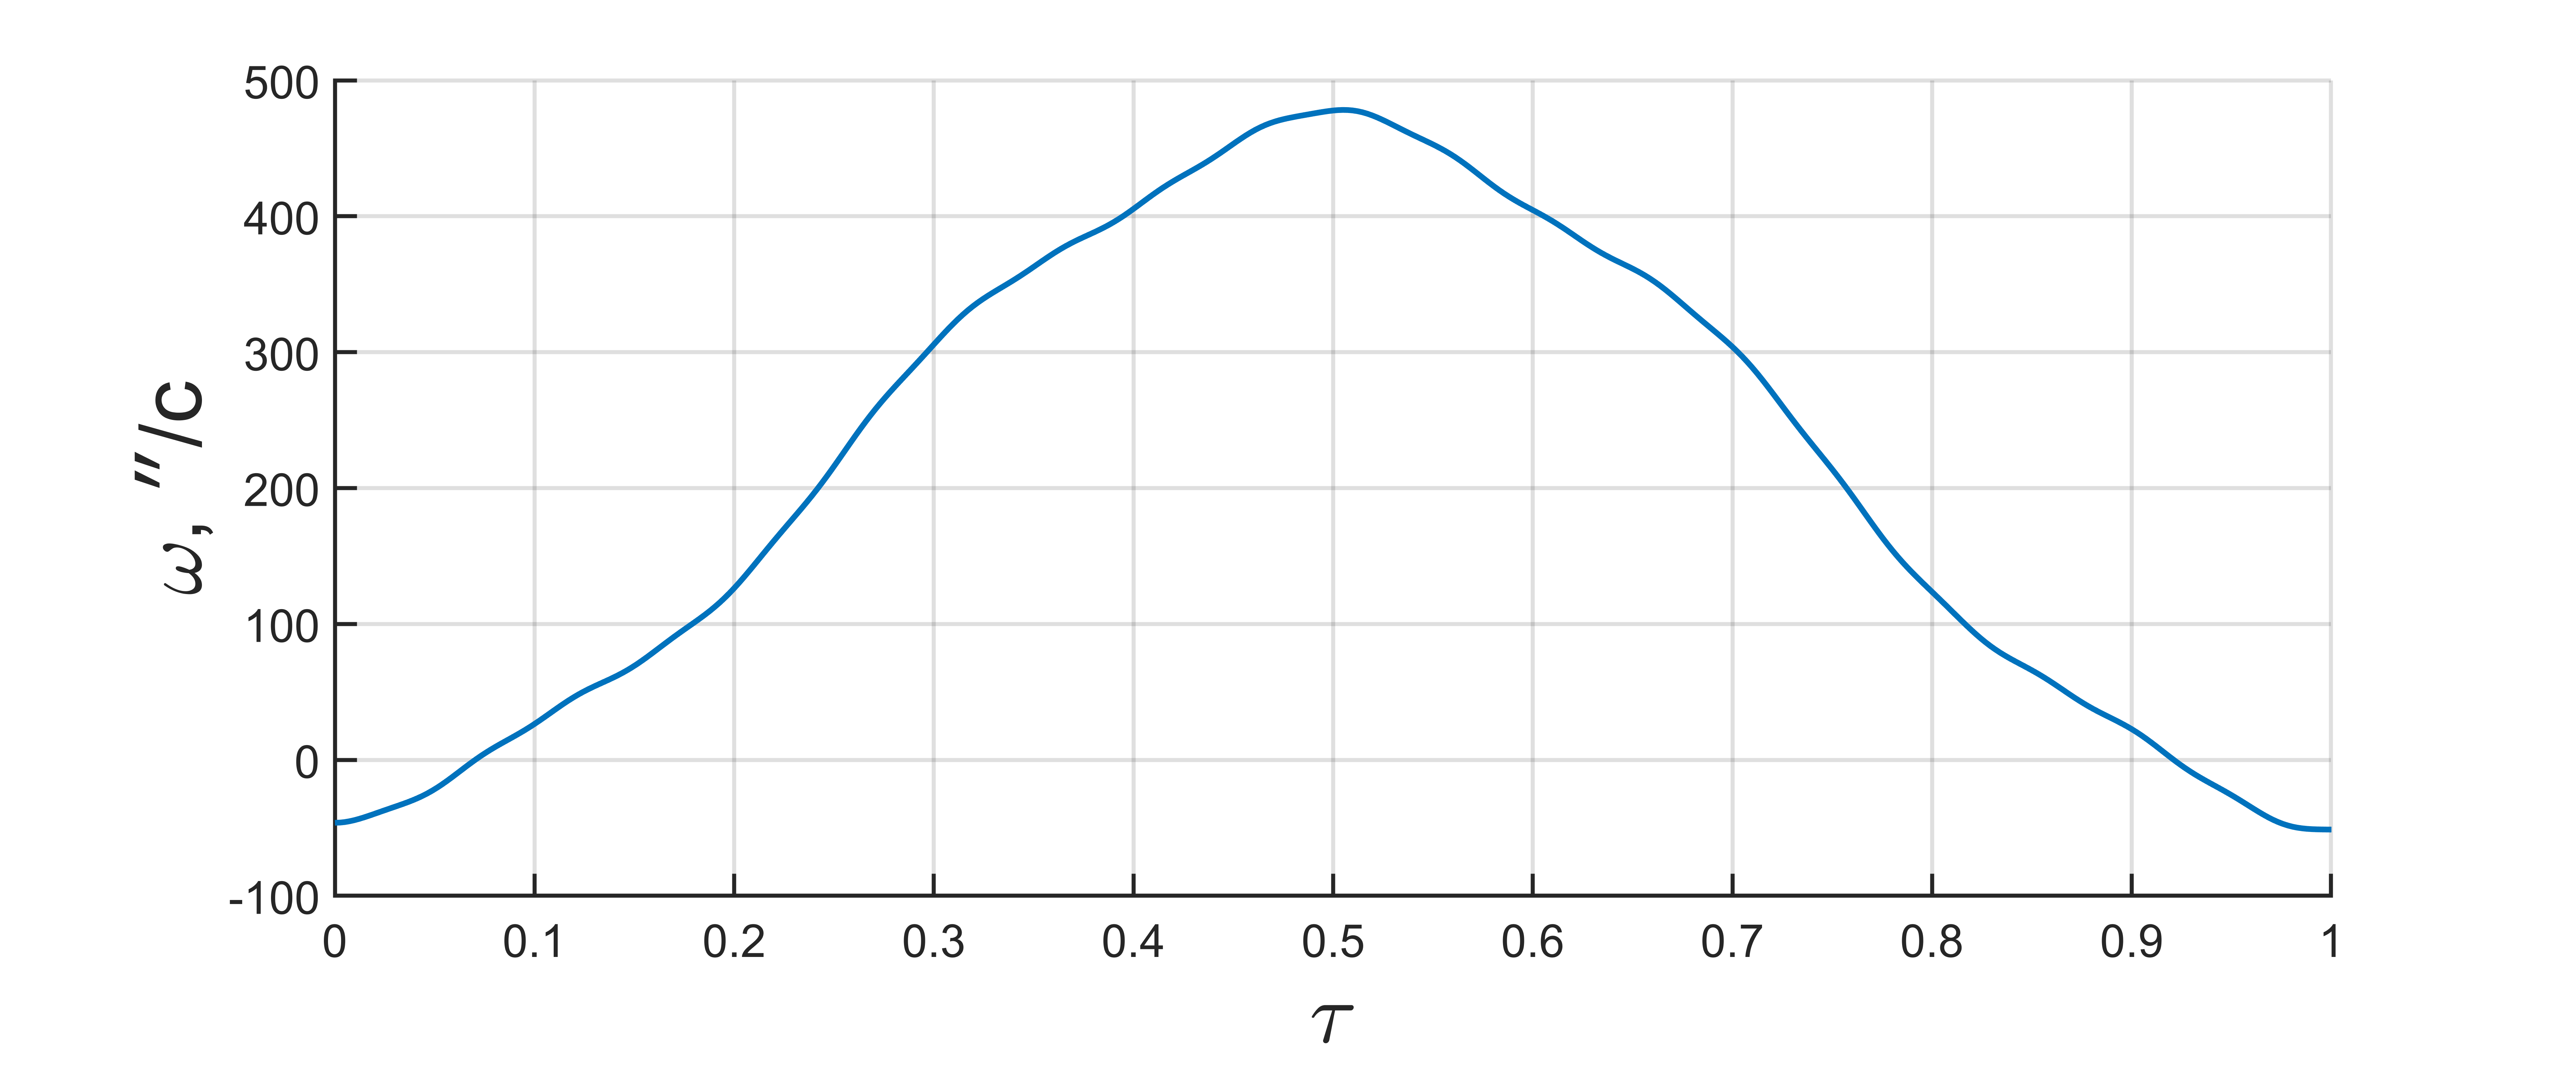
\includegraphics[width=\linewidth]{matlab/img/oy-gyro-sin-vel} \\ б) Угловая скорость (ось $OY$)
	\end{minipage}
	
	\vspace{0.5em} % расстояние между строками
	
	% --- Вторая строка ---
	\begin{minipage}[b]{0.49\linewidth}\centering
		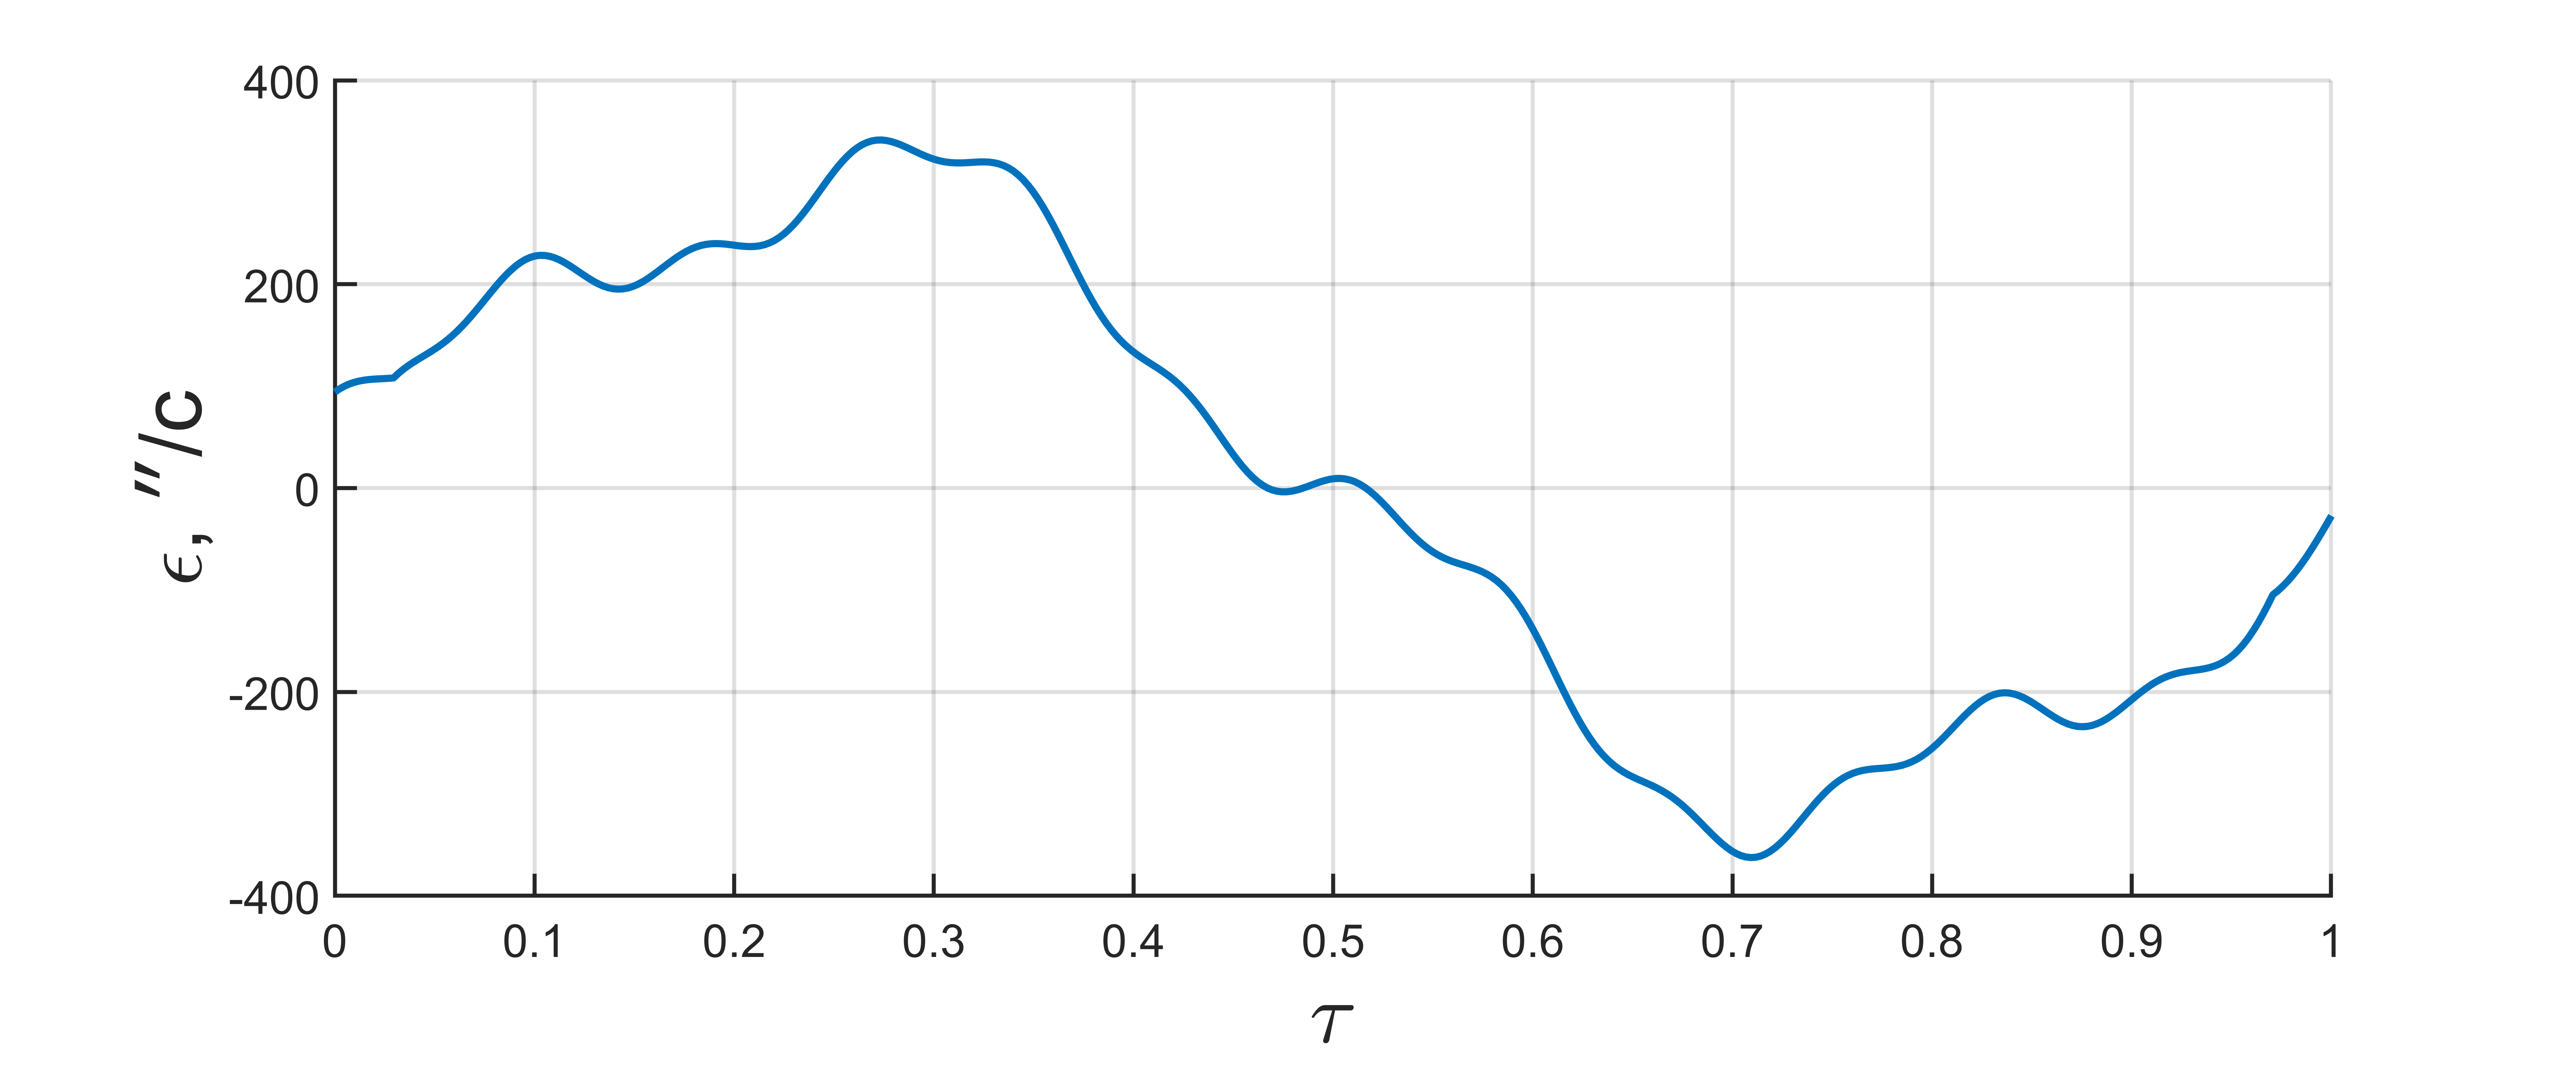
\includegraphics[width=\linewidth]{matlab/img/oz-gyro-sin-acc} \\ в) угловое ускорение (ось $OZ$)
	\end{minipage}
	\hfill
	\begin{minipage}[b]{0.49\linewidth}\centering
		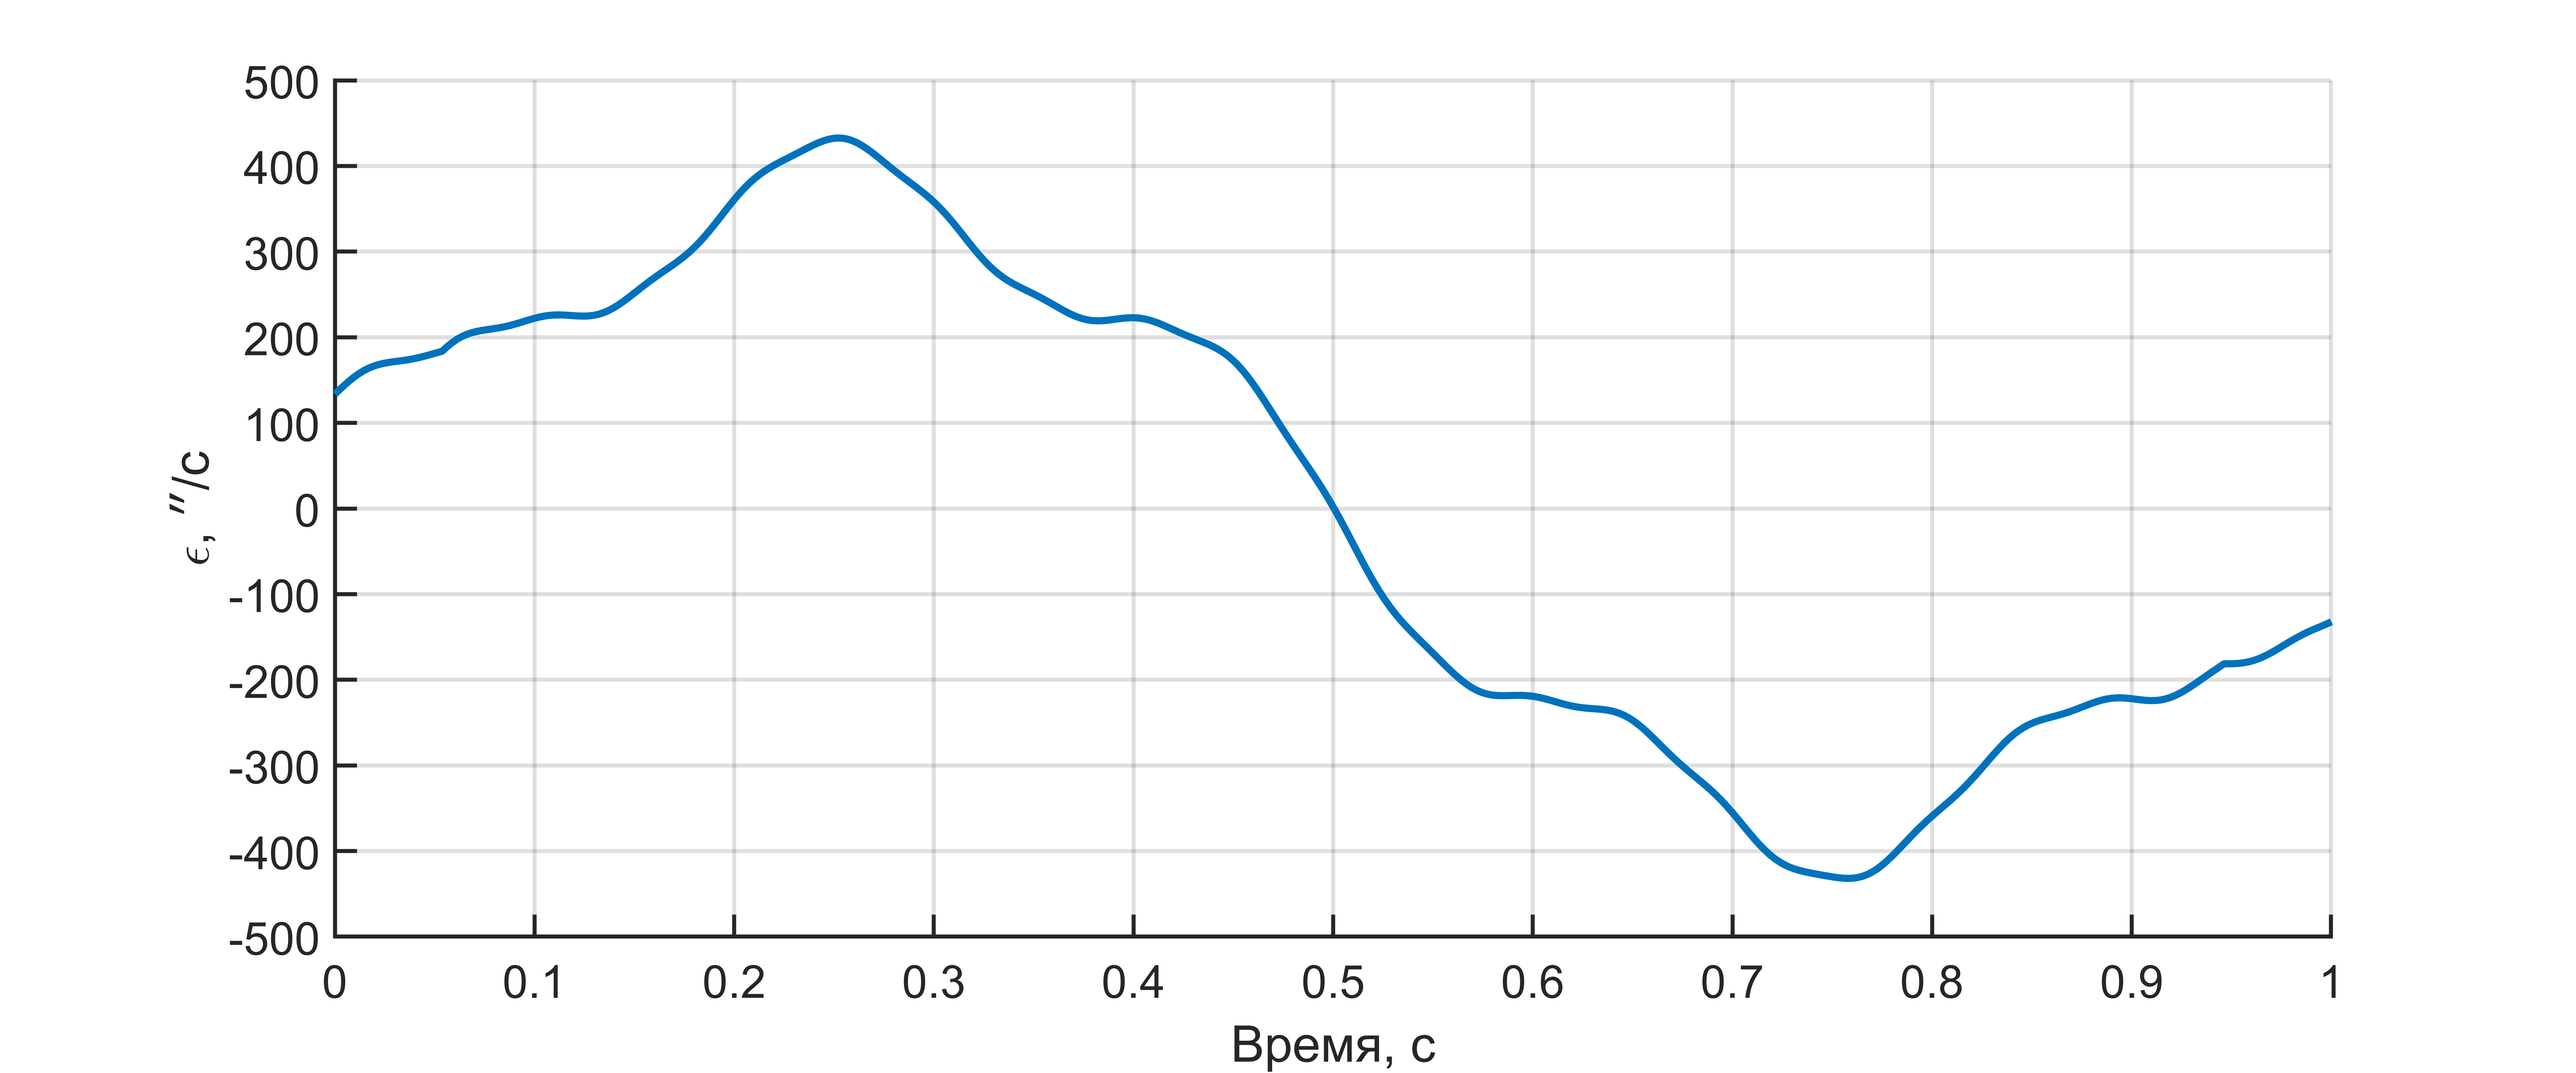
\includegraphics[width=\linewidth]{matlab/img/oy-gyro-sin-acc} \\ г)  угловое ускорение (ось $OY$)
	\end{minipage}
	
	\vspace{0.5em} % расстояние между строками
	
	\begin{minipage}[b]{0.49\linewidth}\centering
	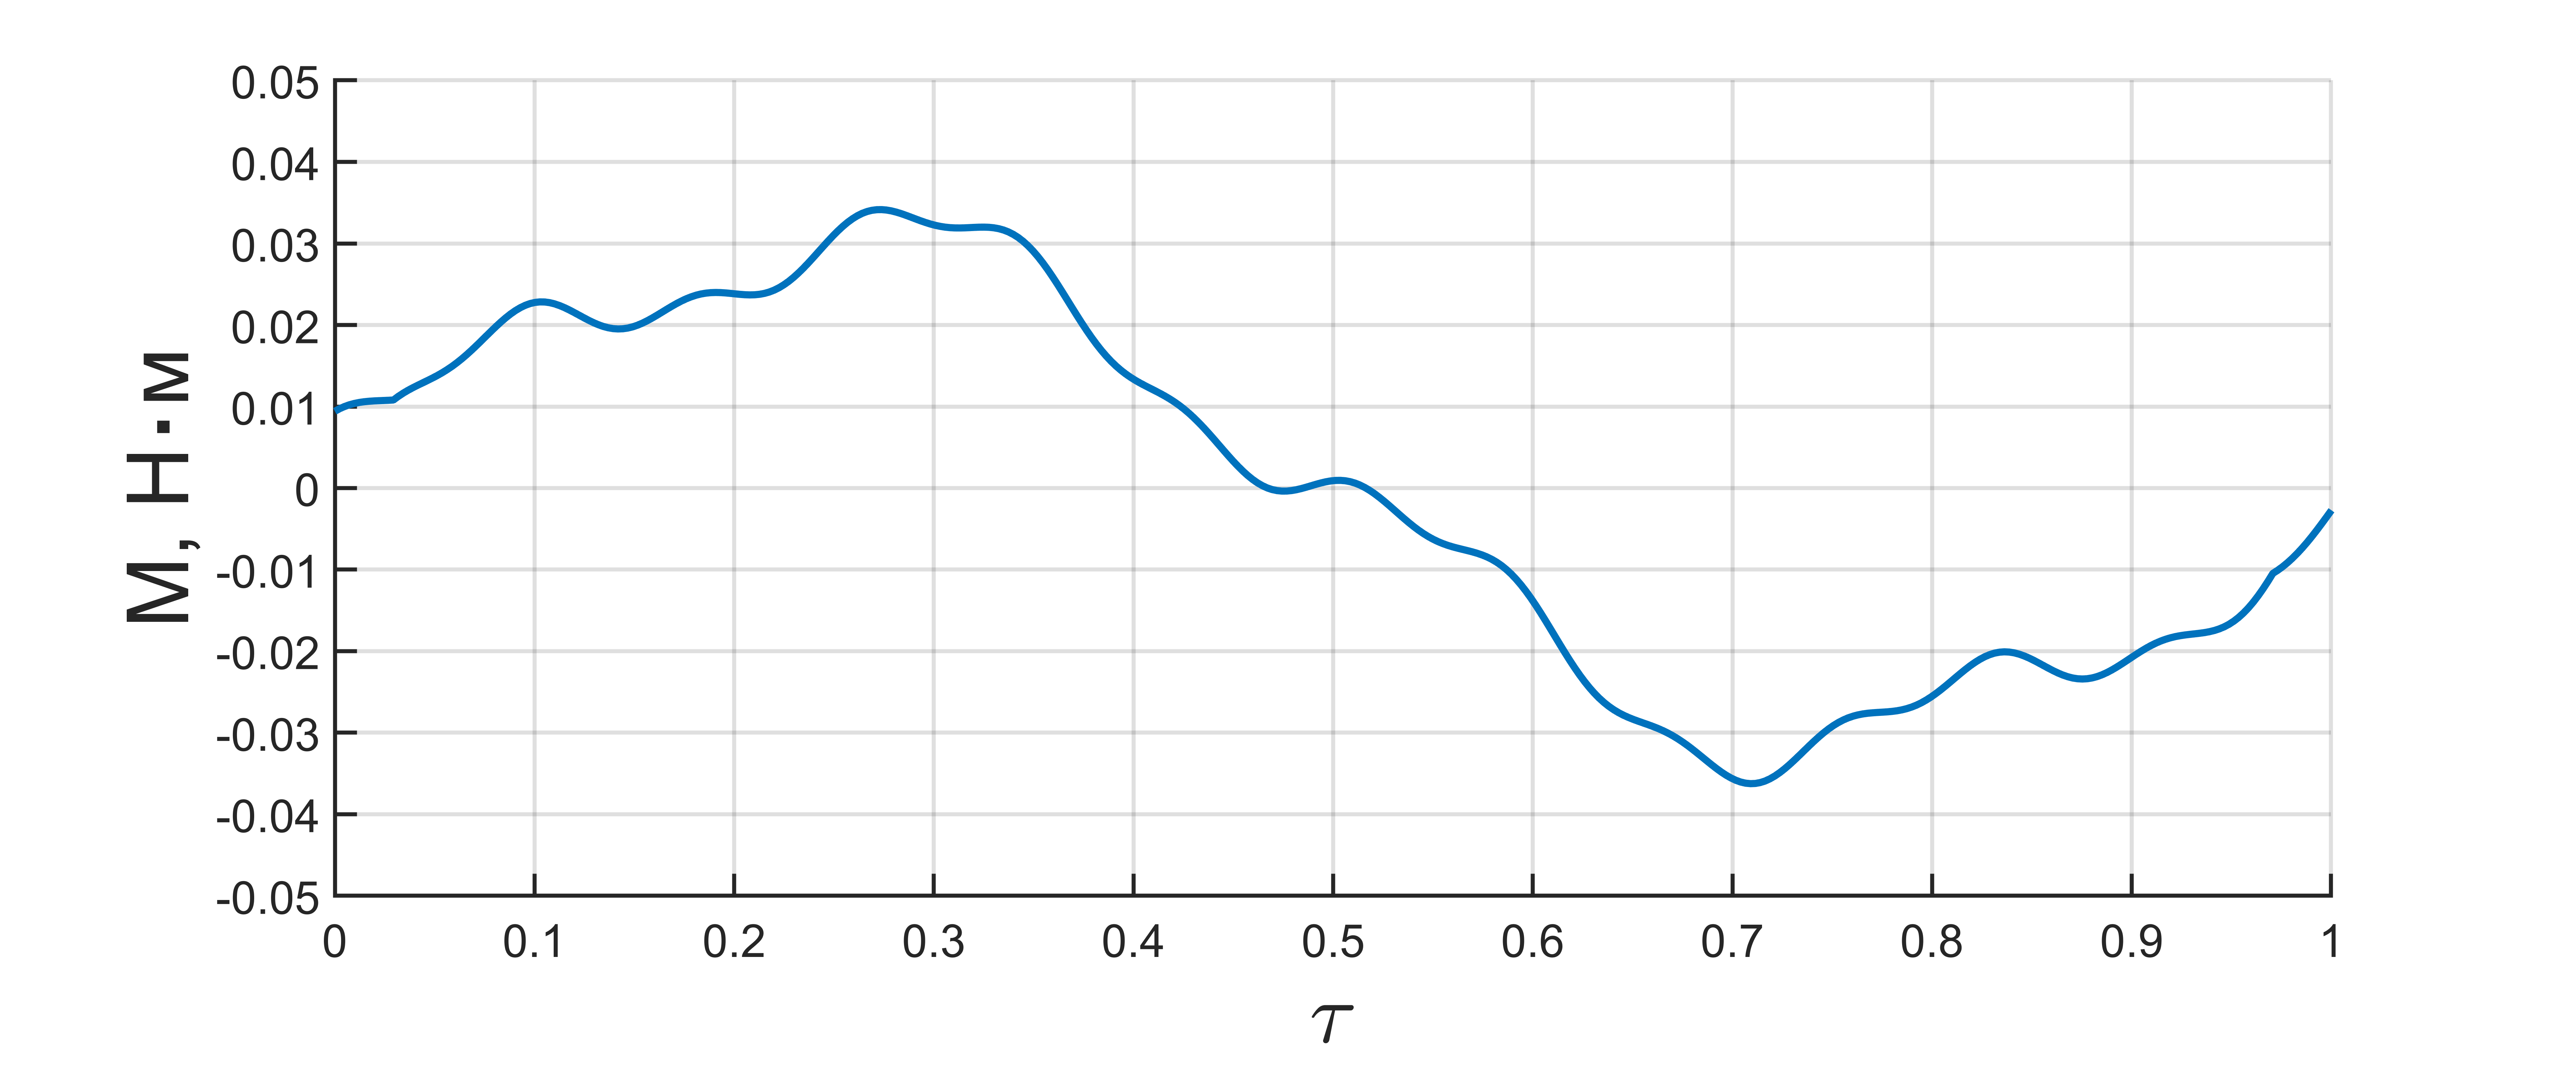
\includegraphics[width=\linewidth]{matlab/img/oz-gyro-sin-mom} \\ д) реактивный момент (ось $OZ$)
	\end{minipage}
	\hfill
	\begin{minipage}[b]{0.49\linewidth}\centering
		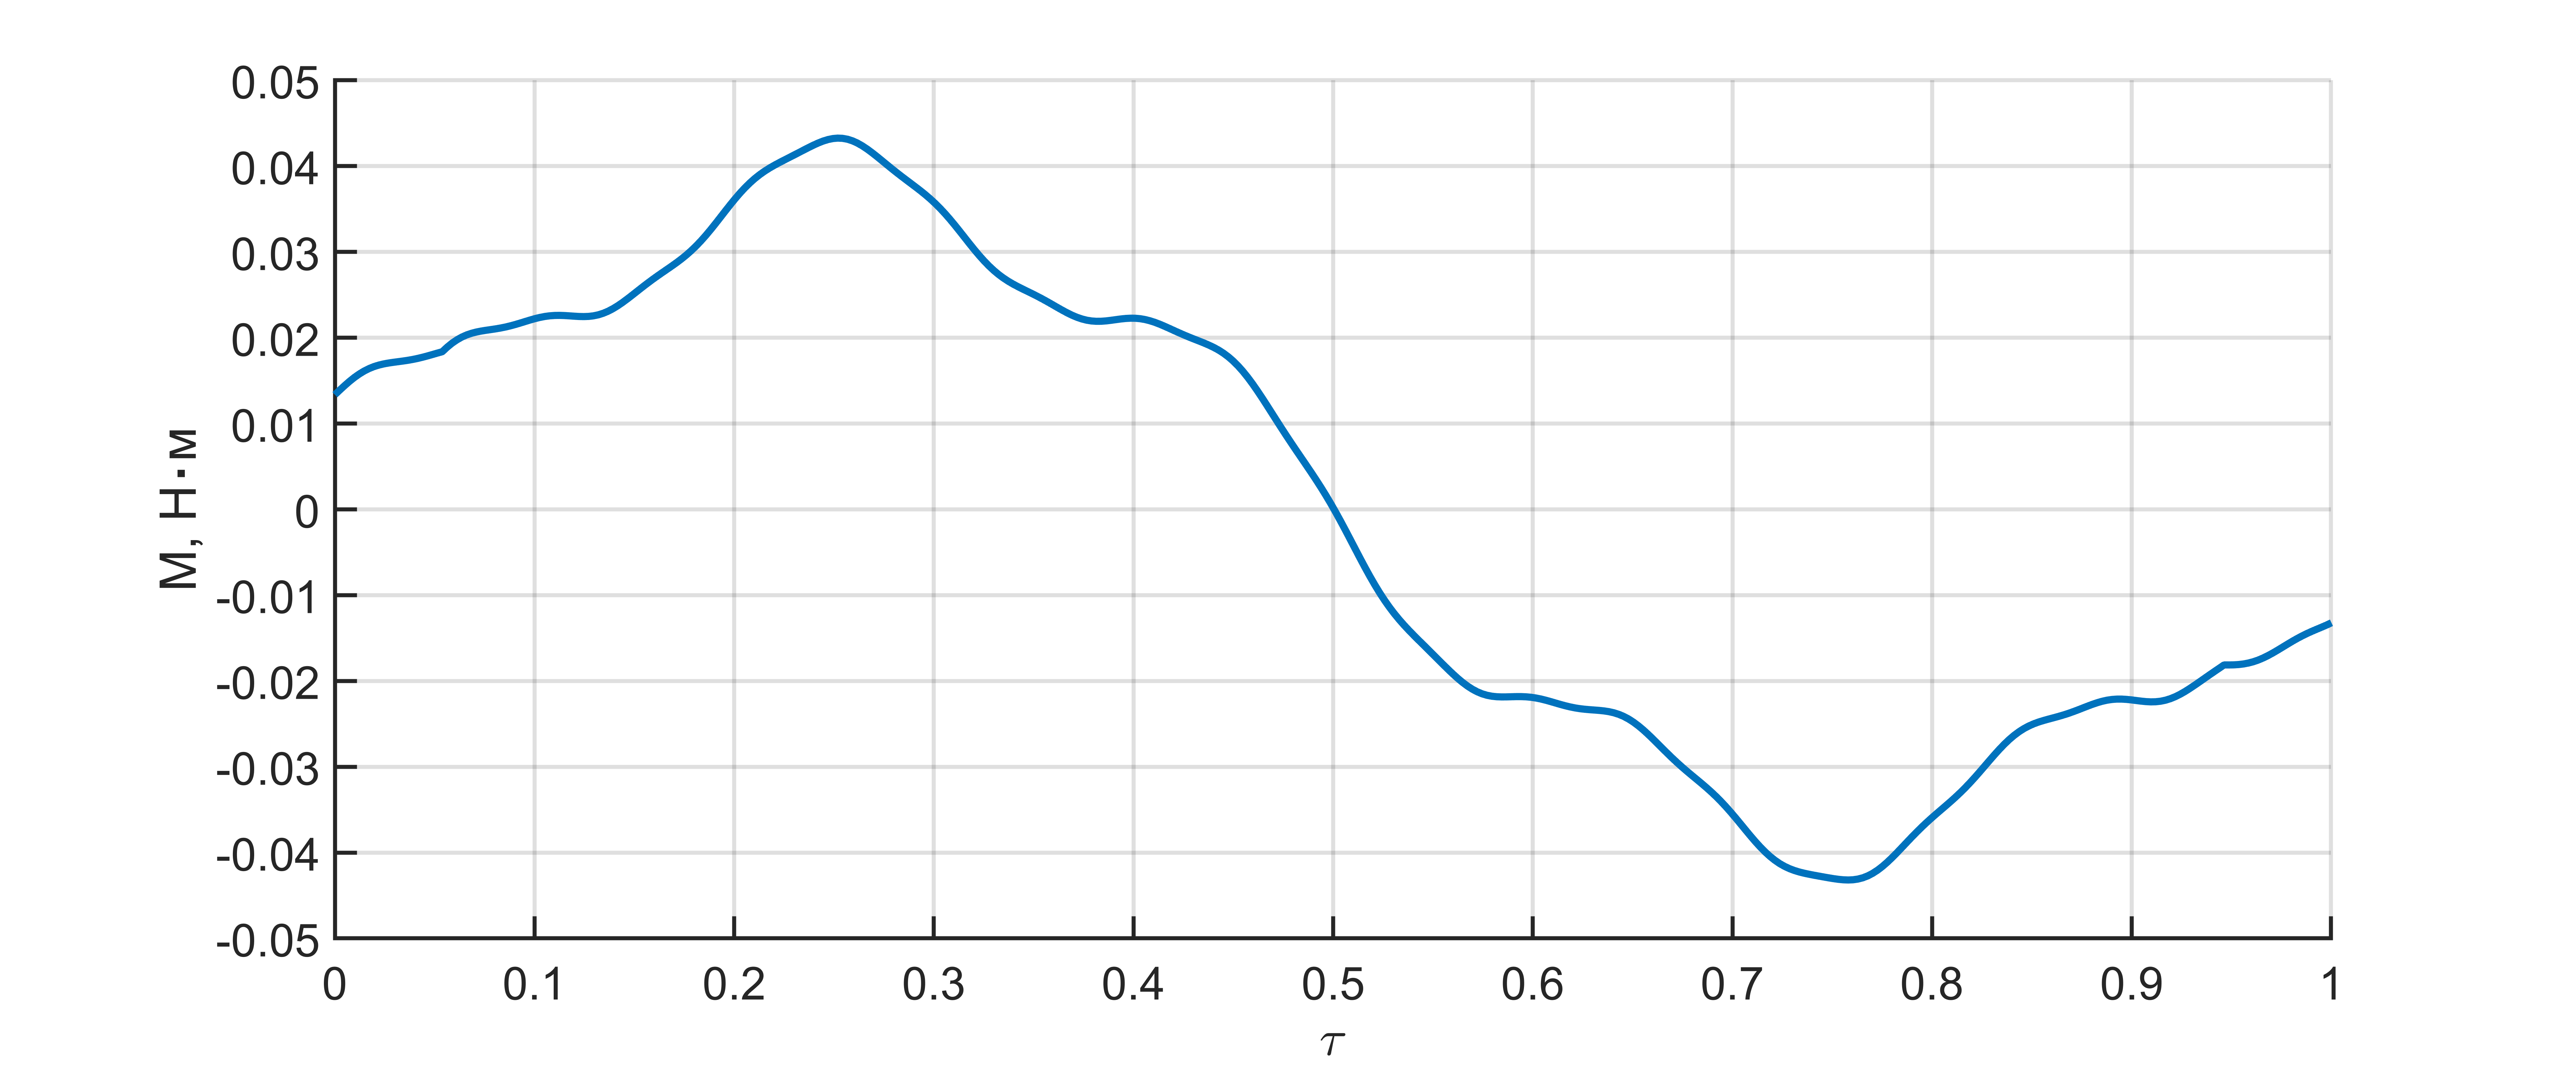
\includegraphics[width=\linewidth]{matlab/img/oy-gyro-sin-mom} \\ е)  реактивный момент (ось $OY$)
	\end{minipage}
	
	\caption{Результаты измерений после установки балансировочных колец}
	\label{fig:sin-profile-omn}
\end{figure}

Сравнение полученных зависимостей с результатами первой серии испытаний показало, что после установки балансировочных колец величина реактивного момента снизилась, а форма кривых стала более симметричной и плавной. Применение синусоидального профиля управления дополнительно уменьшило амплитуду ускорений и сгладило переходные процессы, что привело к снижению возбуждения колебаний подвесной системы. Таким образом, доработанная конструкция МНО в сочетании с оптимизированным законом управления обеспечивает более эффективную компенсацию реактивного момента и повышает точность стабилизации оптической системы.
 
 \section{Анализ влияния остаточного реактивного момента на параметры качества изображения}
 
 На основе параметров, полученных в результате стендовых испытаний, был изготовлен лётный образец ОМУ, интегрированный в состав космического аппарата. Для оценки эффективности улучшенной компенсации в условиях полёта был проведён анализ показаний бортовых гироскопов после выведения КА на орбиту. Данные угловых скоростей спутника послужили исходной информацией для последующего расчёта колебаний и оценки их влияния на качество изображения. На рисунке~\cref{fig:sat_gyro_data} представлены данные бортовых гироскопов, показывающие угловые скорости спутника за длительный период времени. В целом они отражают работу системы ориентации в штатном режиме.
 
 \begin{figure}[h!]
 	\centering
 	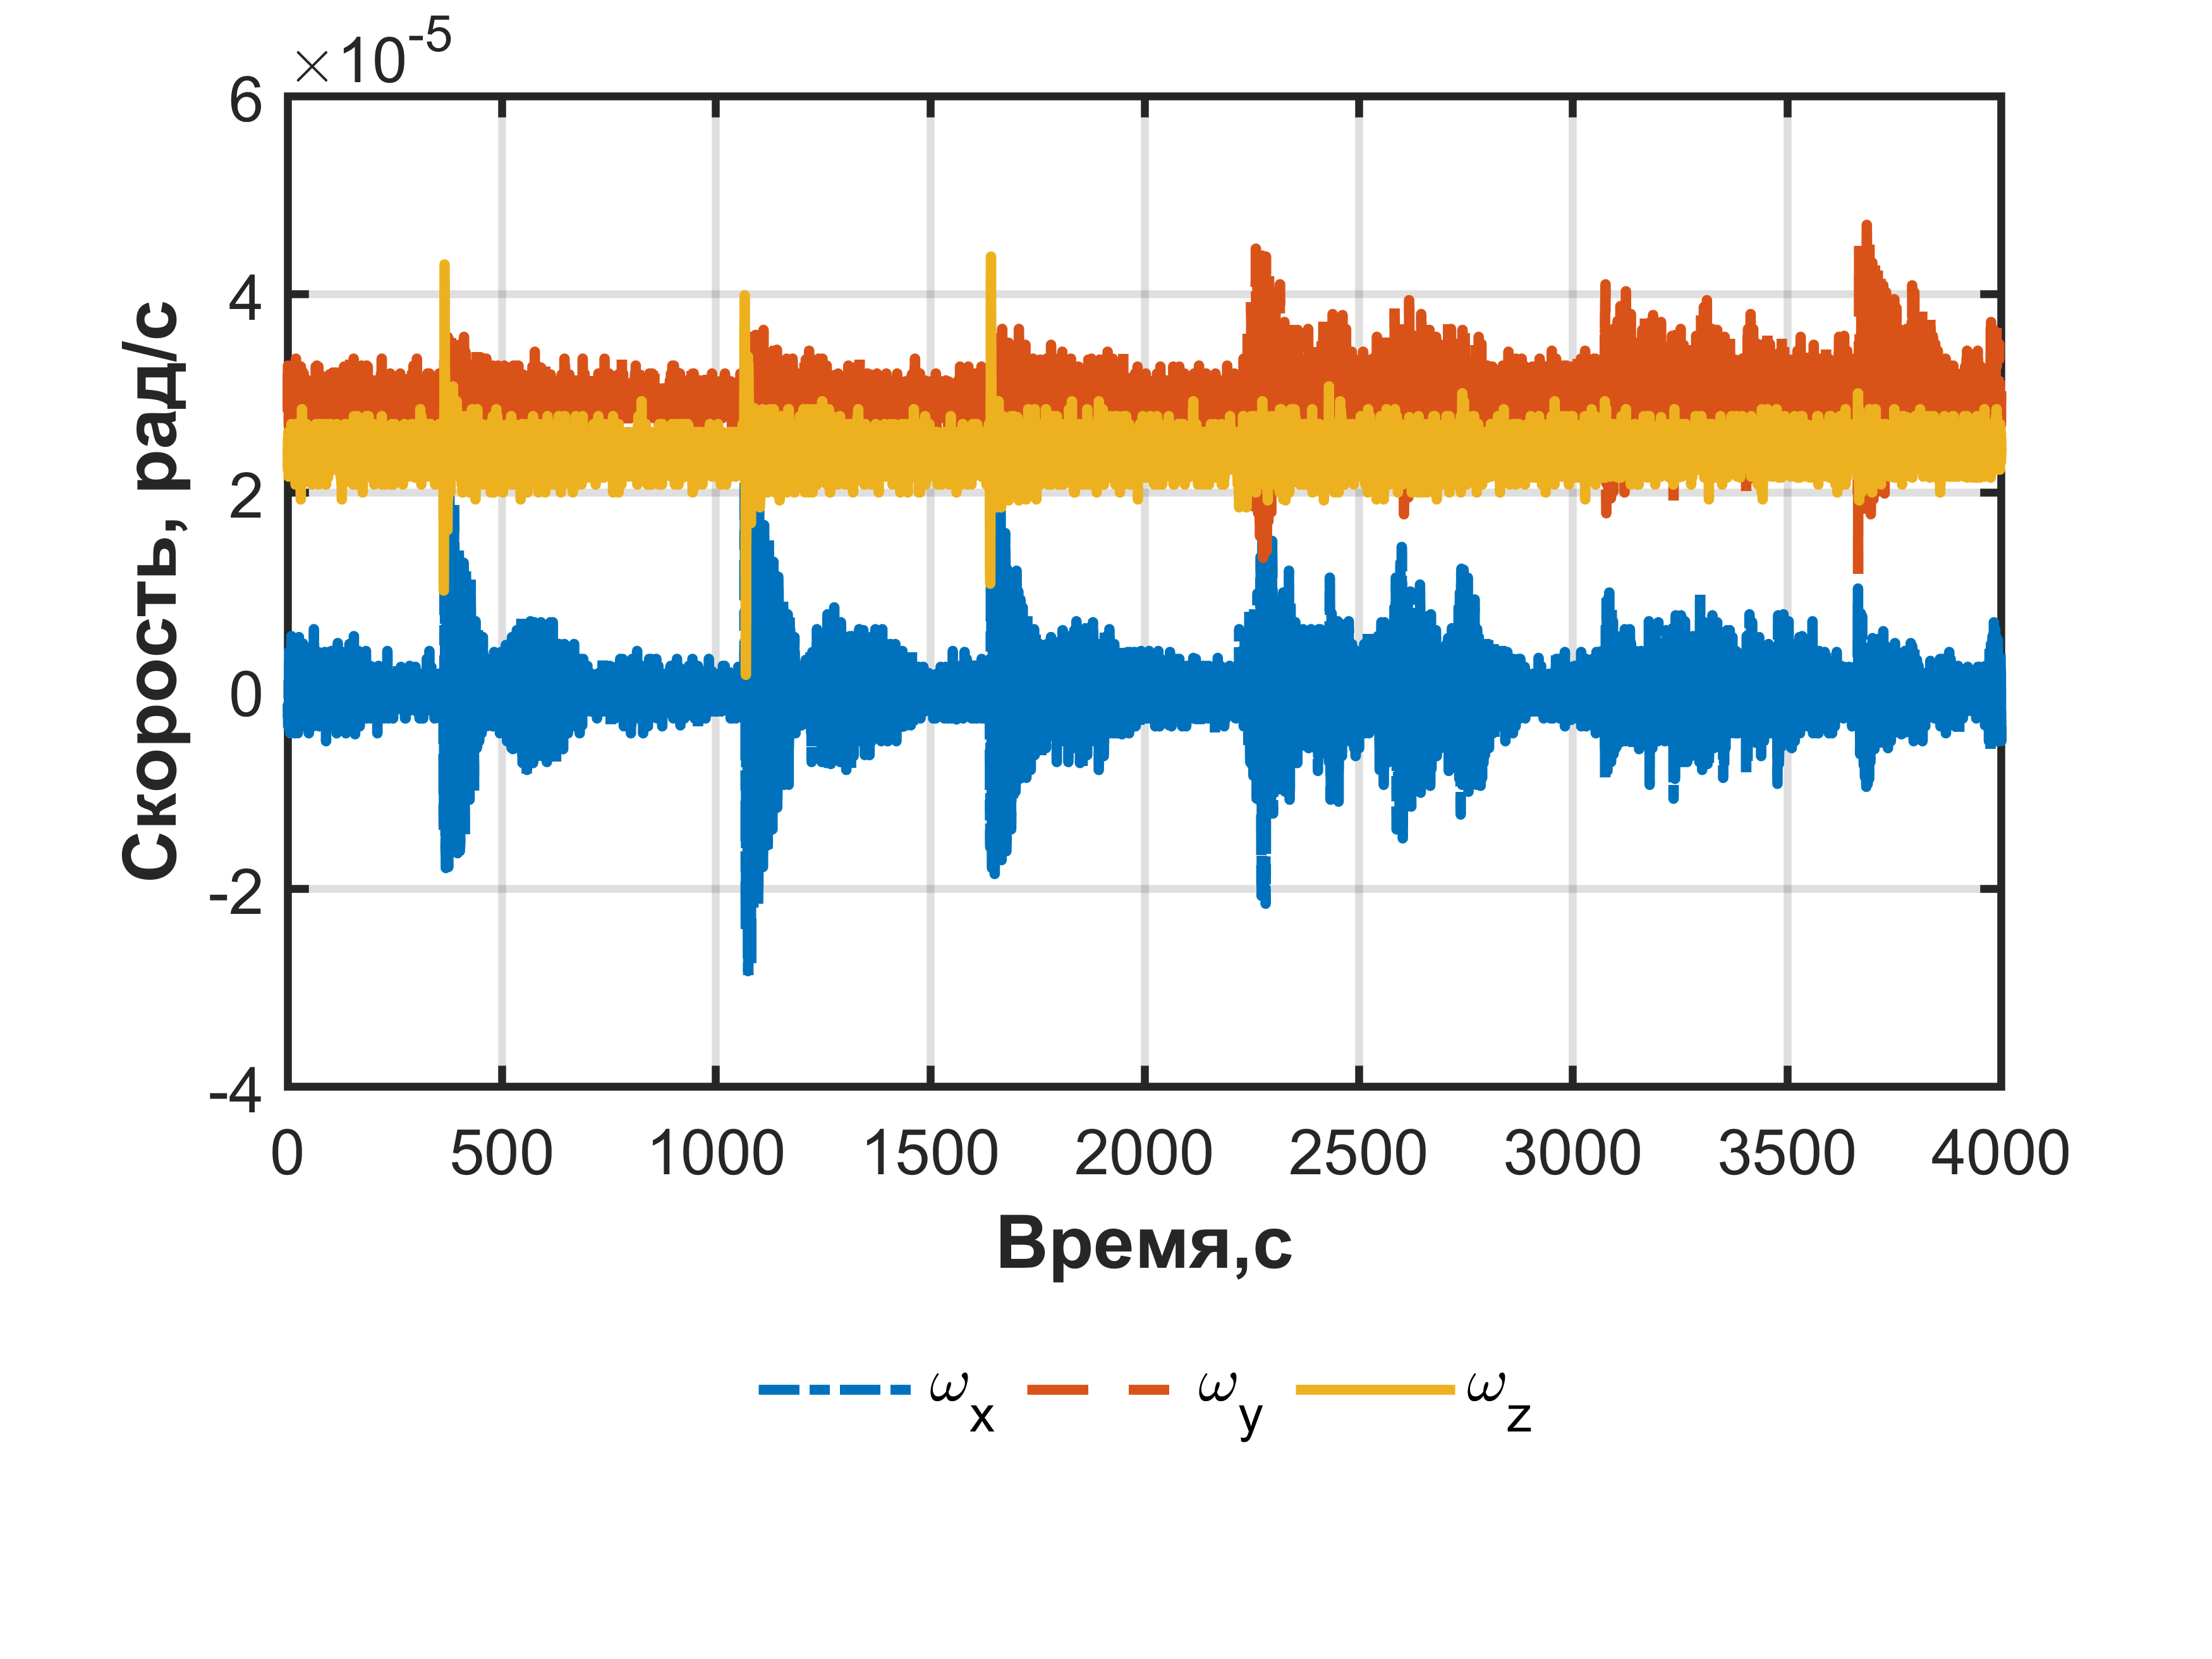
\includegraphics[width=0.8\linewidth]{matlab/img/sat_gyro_data.png}
 	\caption{Данные бортовых гироскопов}
 	\label{fig:sat_gyro_data}
 \end{figure}
 
 Для анализа были выделены интервалы, в которых ось визирования поворачивалась на максимально возможные углы. Именно в эти моменты реактивные моменты достигают наибольших значений. Графики угловых скоростей при повороте оси визирования представлены на рисунке ~\cref{fig:rotationYZ}.
 
 \begin{figure}[h!]
 	\begin{minipage}[b][][b]{0.49\linewidth}\centering
 		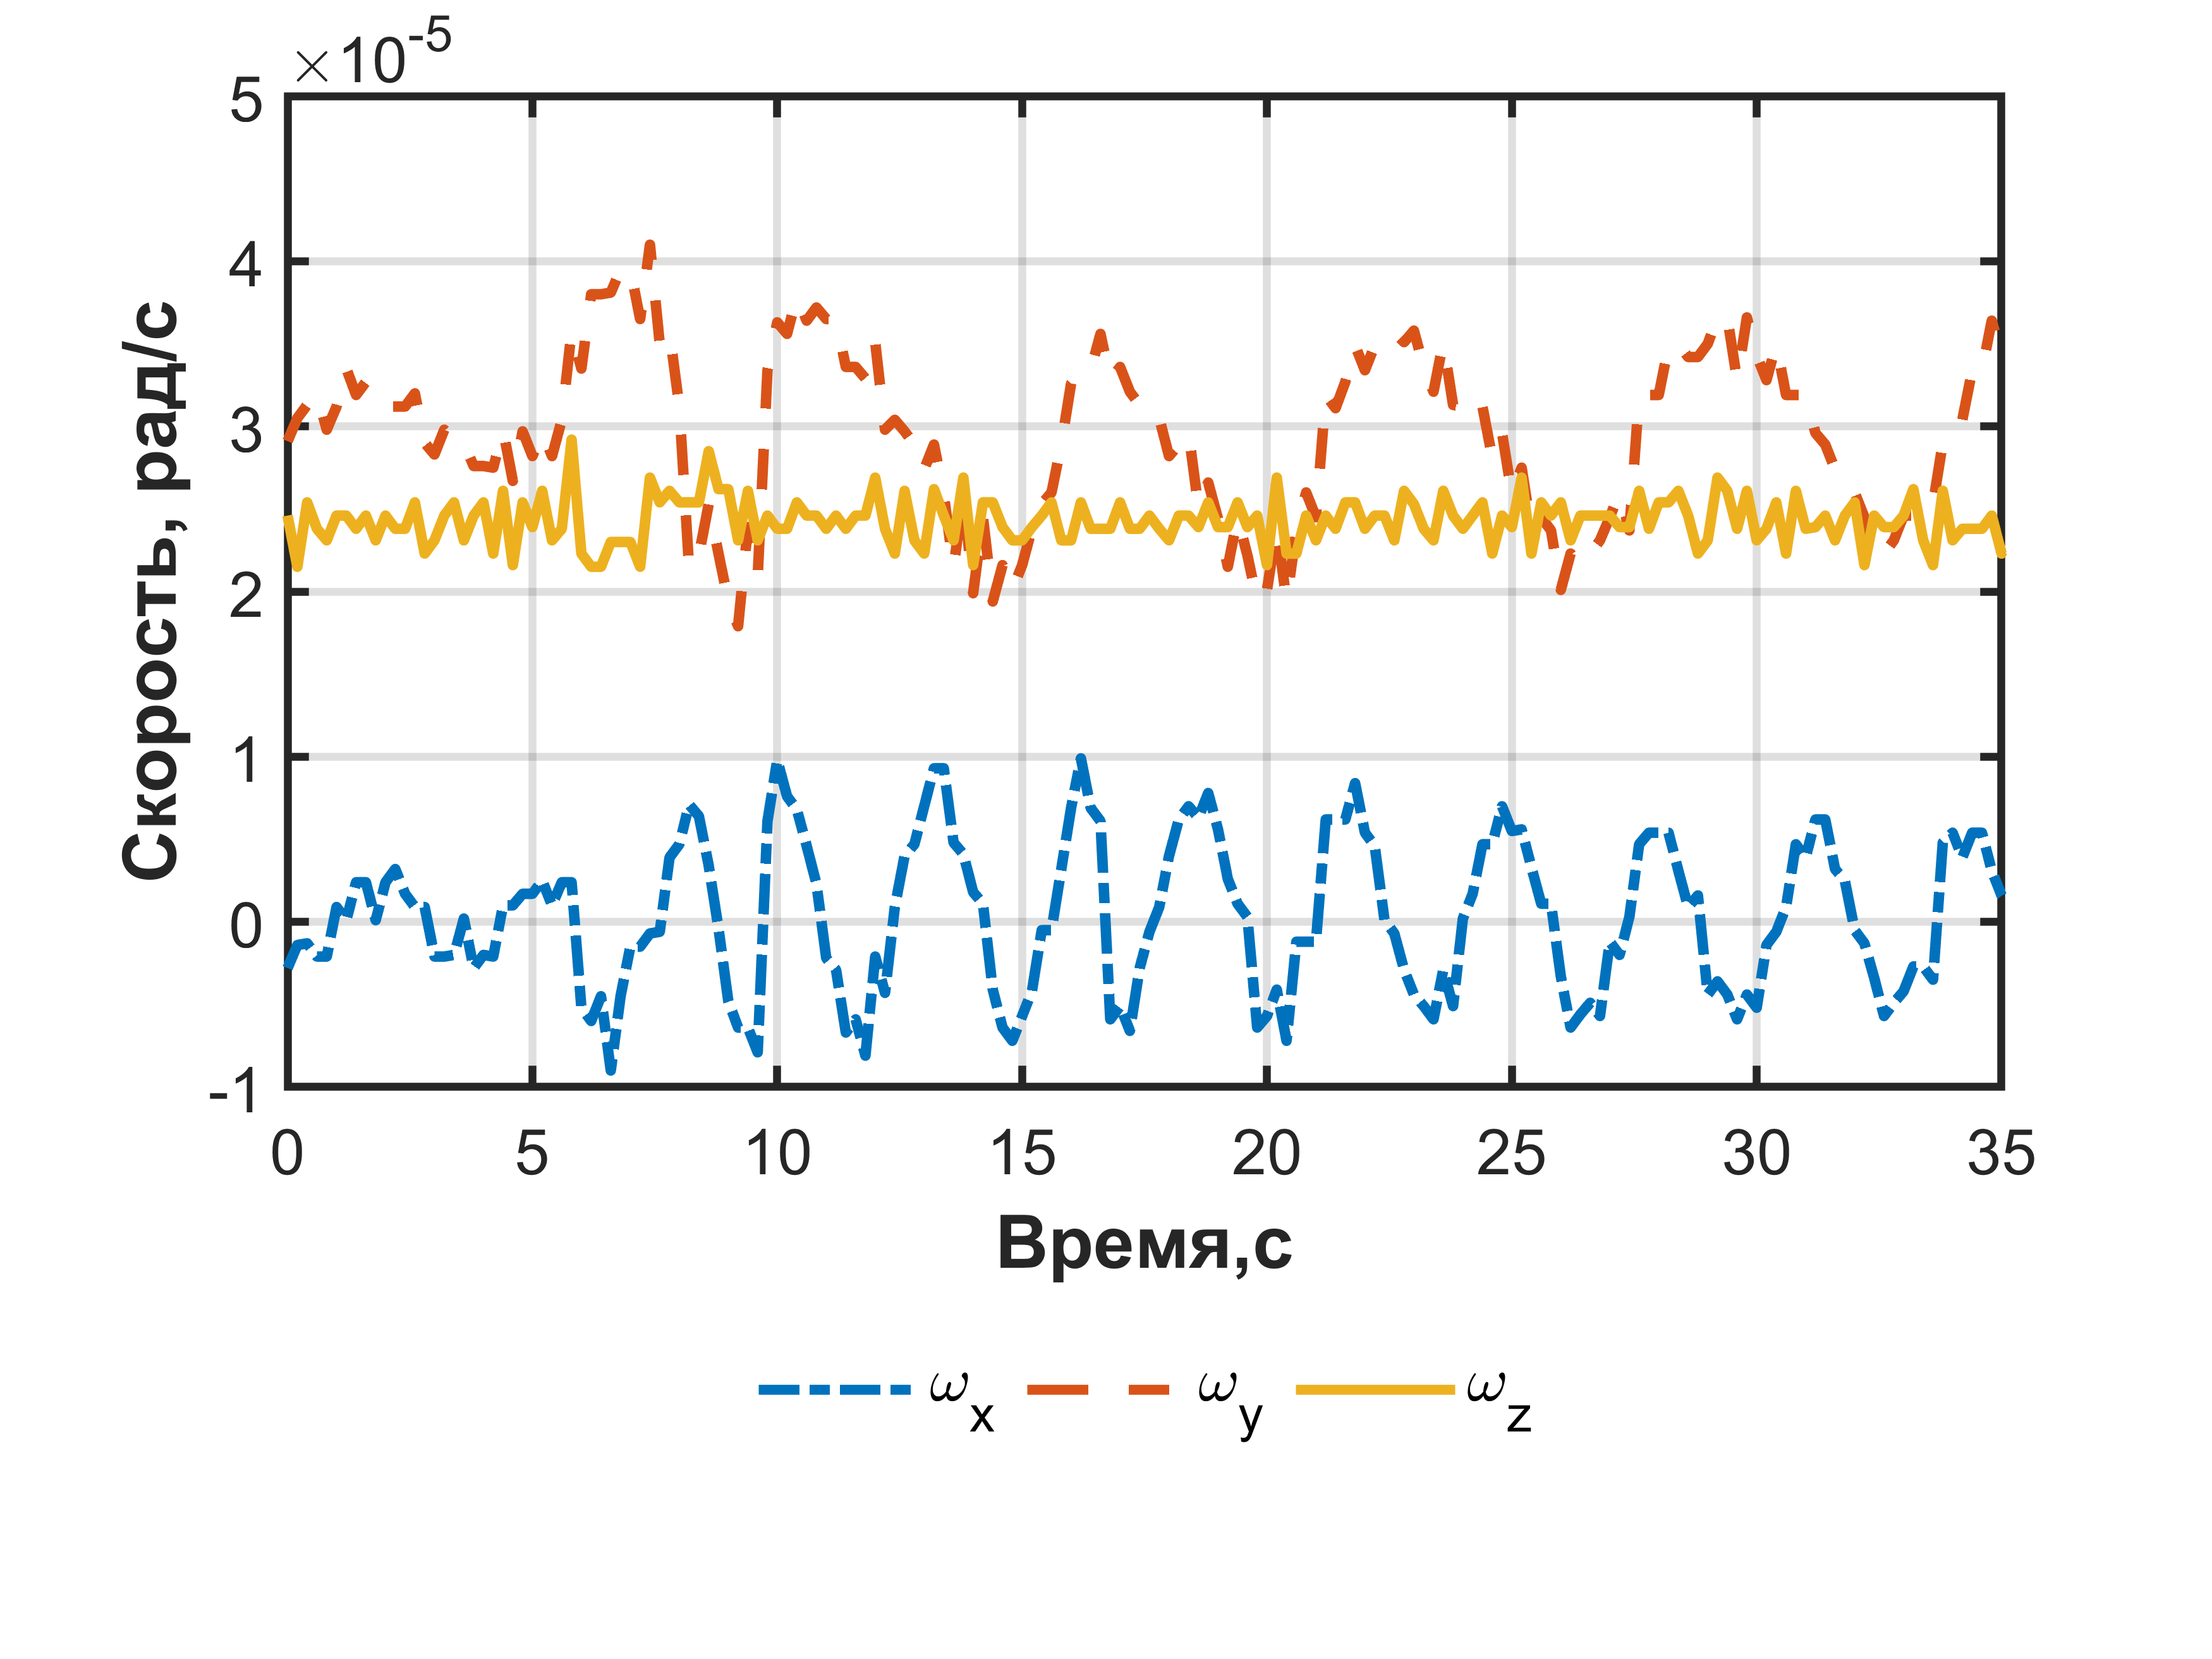
\includegraphics[width=1\linewidth]{matlab/img/sat_gyro_dataY.png} \\ a)
 	\end{minipage}
 	\hfill
 	\begin{minipage}[b][][b]{0.49\linewidth}\centering
 		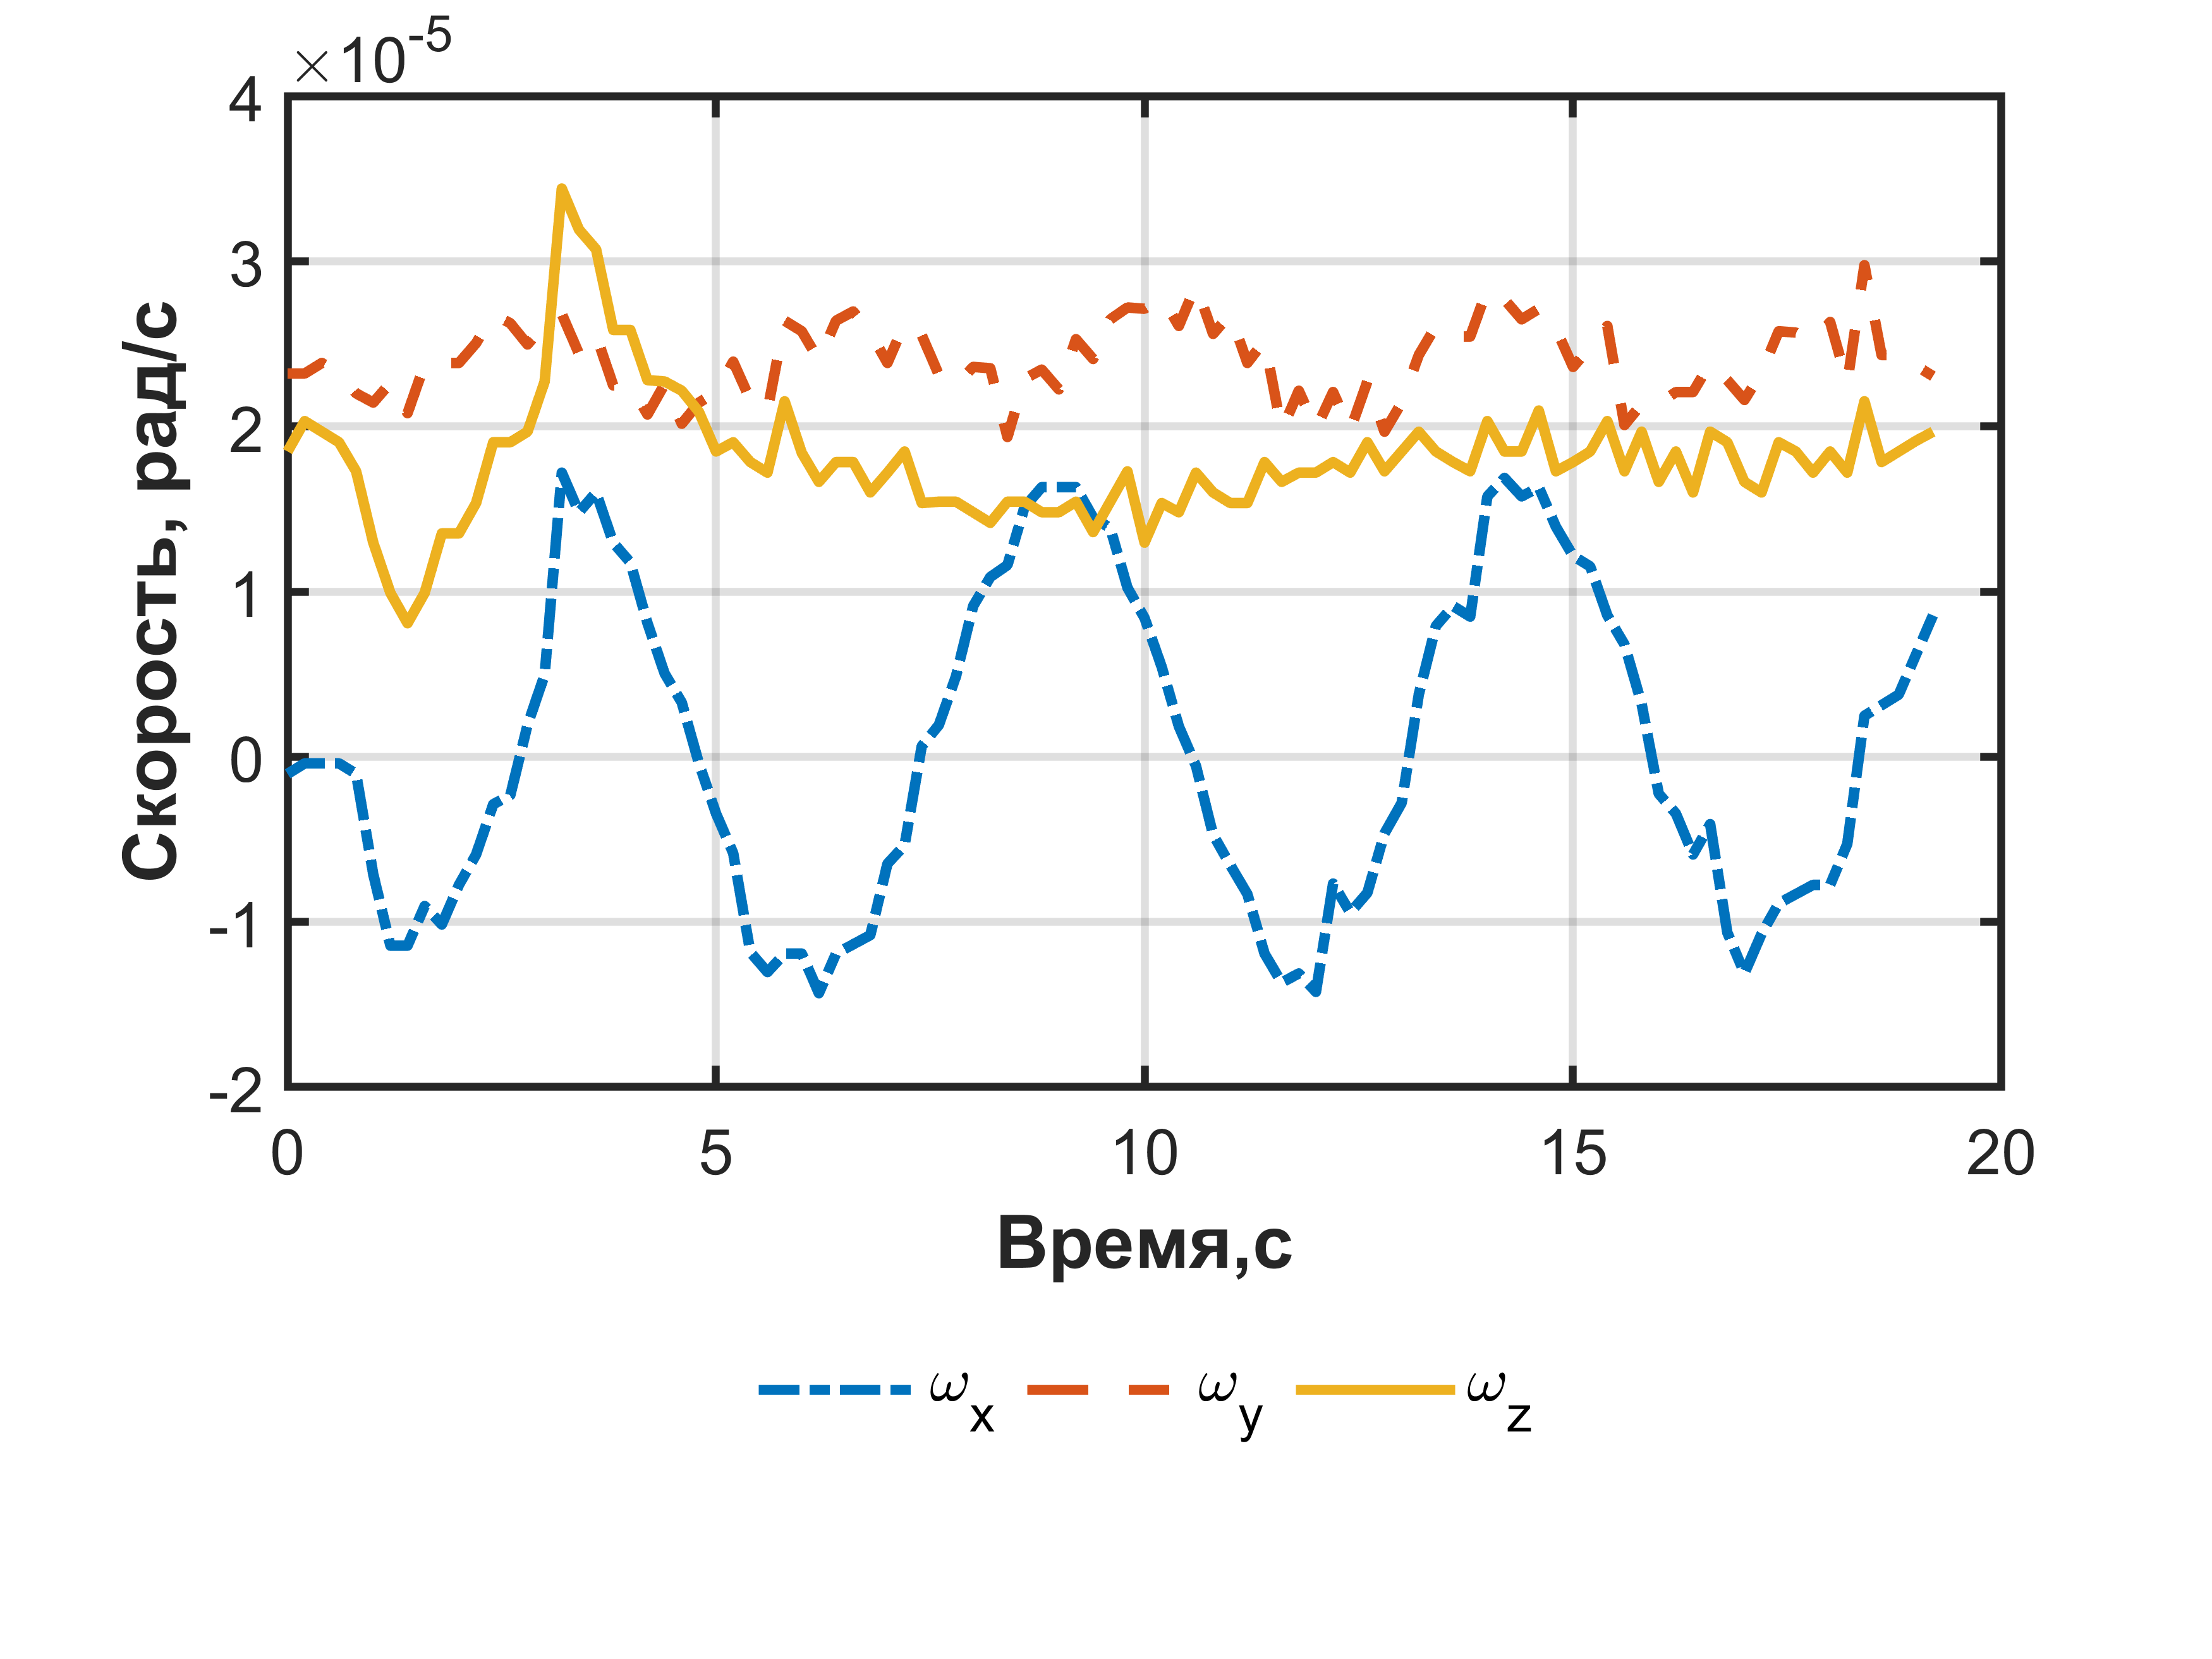
\includegraphics[width=1\linewidth]{matlab/img/sat_gyro_dataZ.png} \\ б)
 	\end{minipage}
 	\caption{Скорость угловых колебаний спутника при повороте оси визирования по a) оси $OY$, б) оси $OZ$ }
 	\label{fig:rotationYZ}
 \end{figure}
 
 Так как ось $OX$ совпадет с оптической осью -- вращение вокруг $OX$ не приводит к параллельному смещению изображения и, соответственно, не формирует линейный \blur{}. Однако, вращение вокруг оси $OX$ создает угловой \blur{} (поворот изображения), величина, которая зависит от положения в поле. За время экспозиции точка на расстоянии $r$ от центра кадра смещается на величину $r\cdot \theta_x$, где $\alpha$ -- угол поворота за время экспозиции. В центре поля ($r=0$) вклад от вращения отсутствует, на краю поля он максимален, $r=R$, где $R$ -- радиус изображения объектива, $\SI{30}{\milli\meter}$.
 
 По измеренным угловым скоростям были получены и использованы углы $\theta_y$, $\theta_z$, отвечающие за трансляцию изображения в плоскости фокуса~\eqref{eq:thetaZY} и $\theta_x$ отвечающий за поворот изображения~\eqref{eq:thetaX}. Угловое перемещение спутника показано на рисунке~\cref{fig:theta}.
 
 \begin{equation}
 	\label{eq:thetaZY}
 	\theta_{y}(t)= \int \omega_{y}\, dt \quad \theta_z(t) = \int \omega_z\,dt
 \end{equation}
 
 \begin{equation}
 	\label{eq:thetaX}
 	\theta_{x}(t)= \int \omega_{x}\, dt 
 \end{equation}
 
 
 \begin{figure}[!h]
 	\begin{minipage}[b][][b]{0.49\linewidth}\centering
 		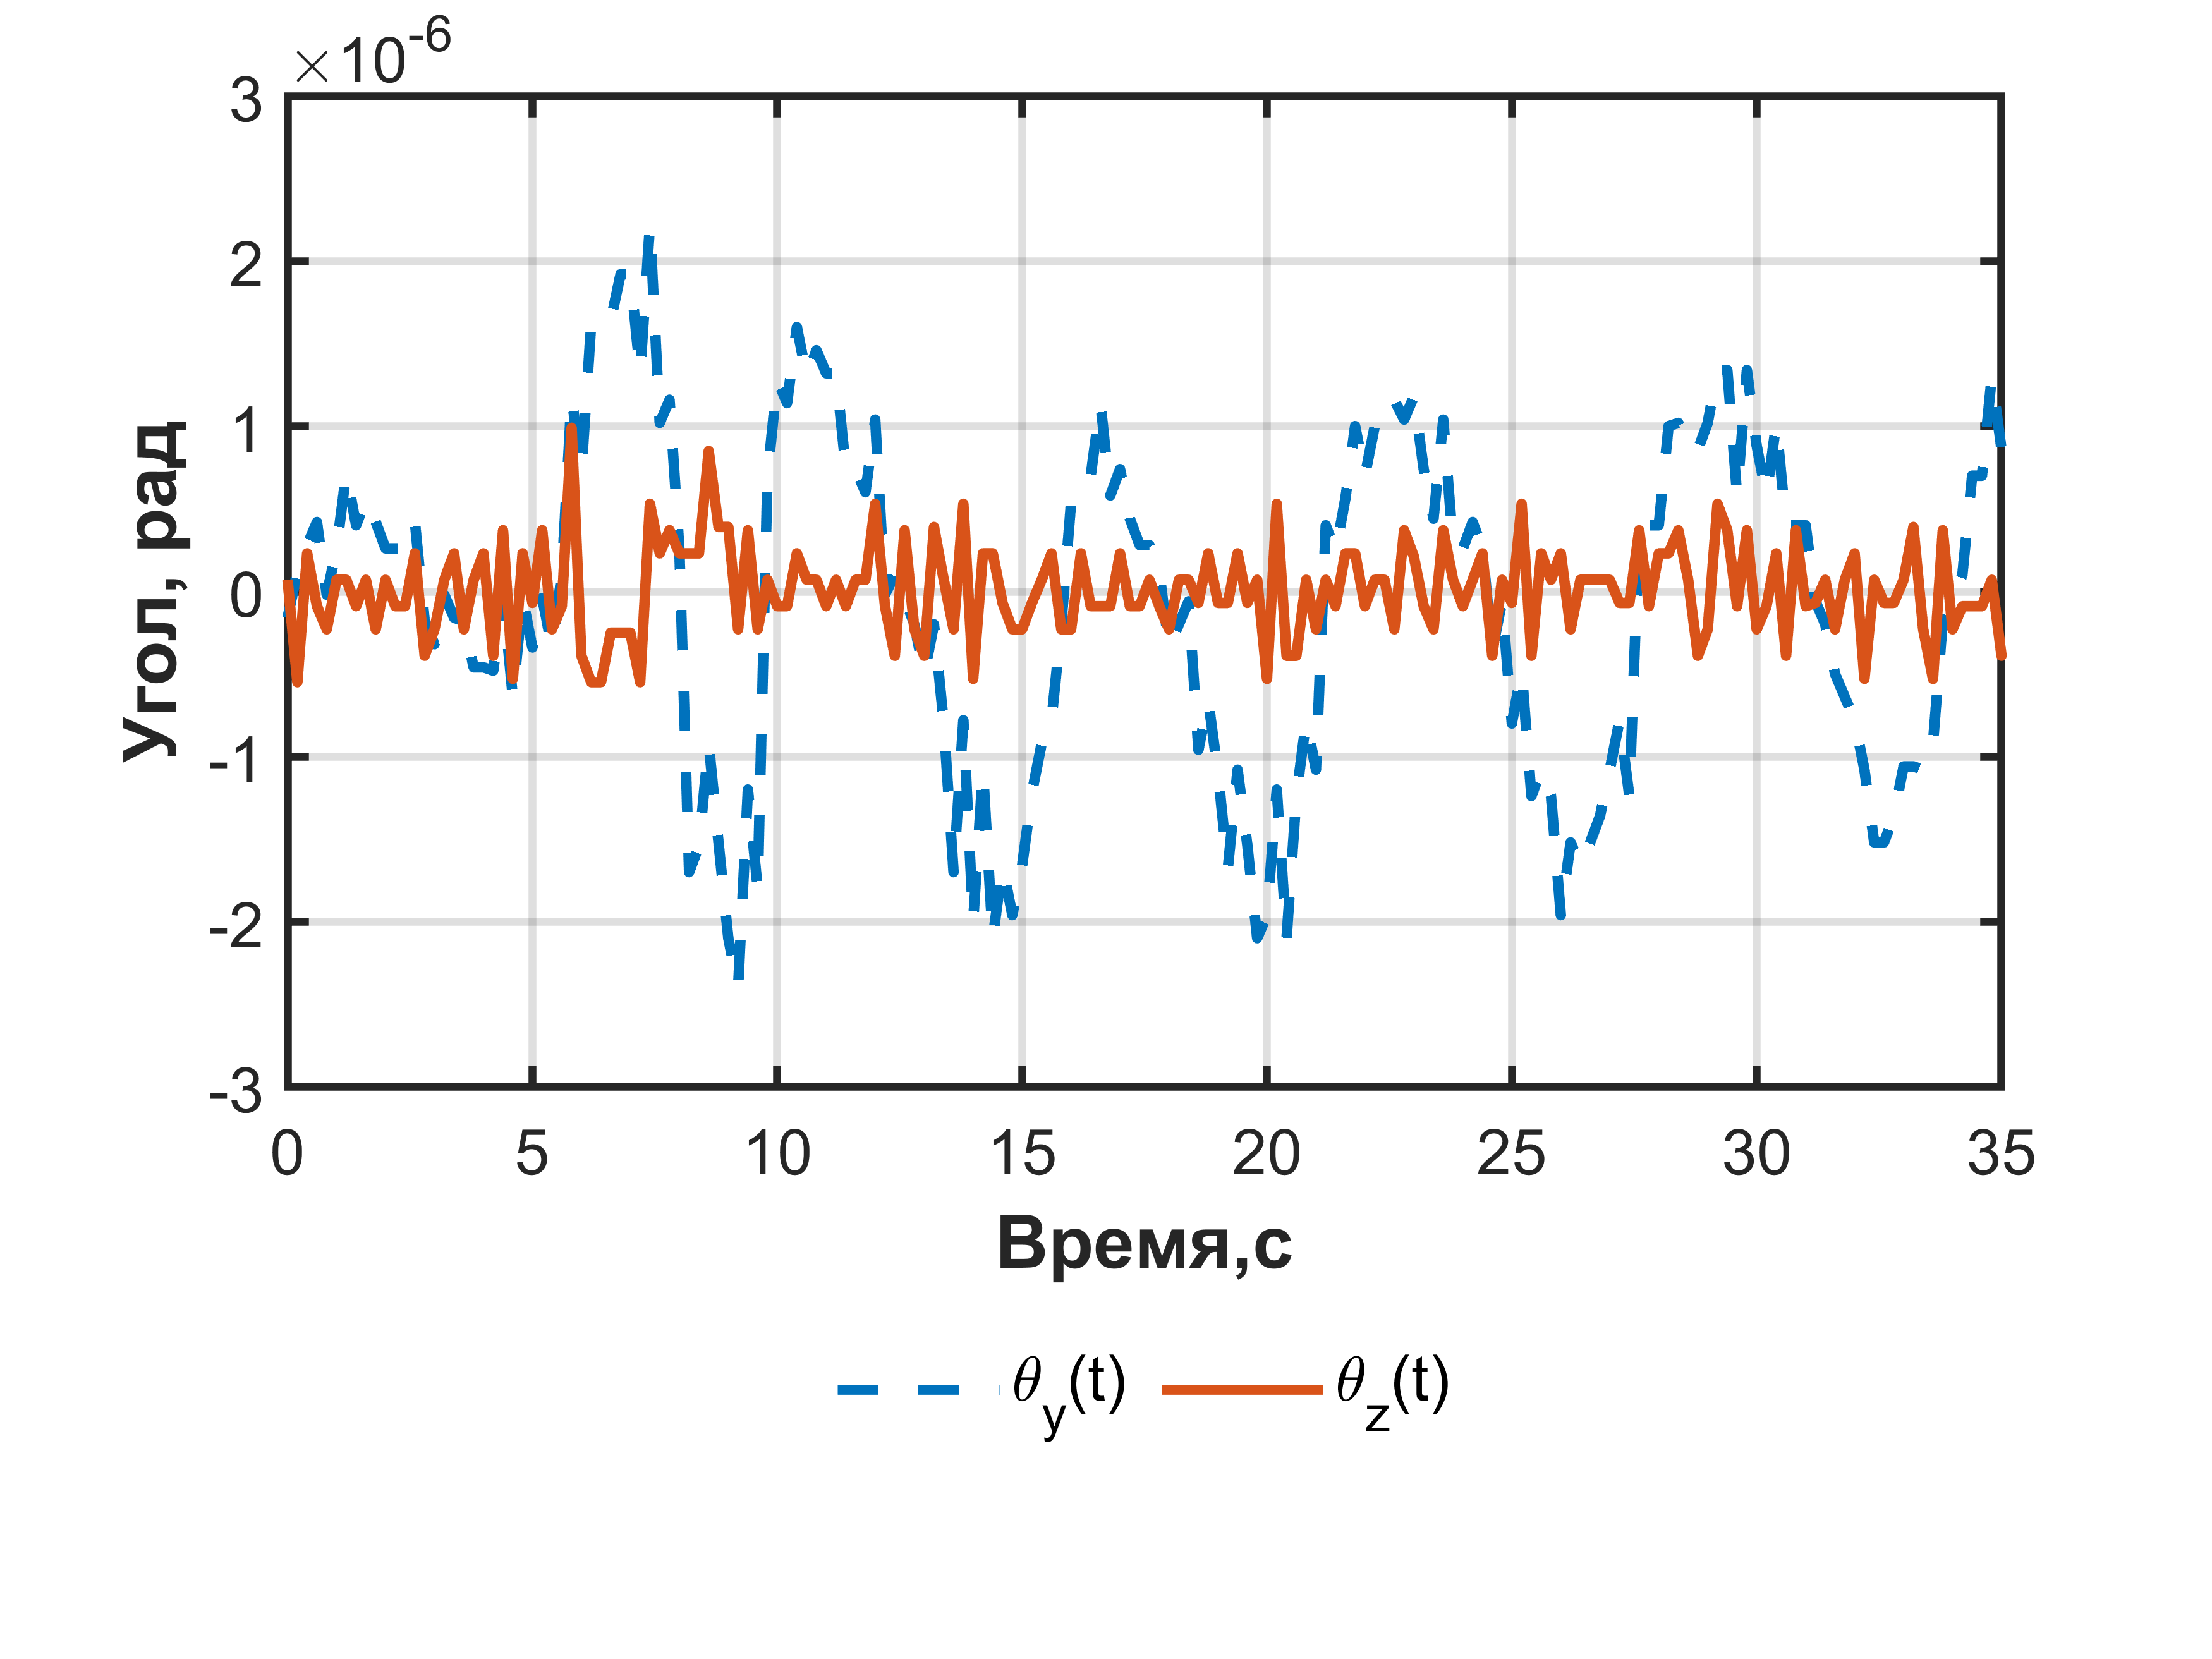
\includegraphics[width=1\linewidth]{matlab/img/thetaY.png} \\ a)
 	\end{minipage}
 	\hfill
 	\begin{minipage}[b][][b]{0.49\linewidth}\centering
 		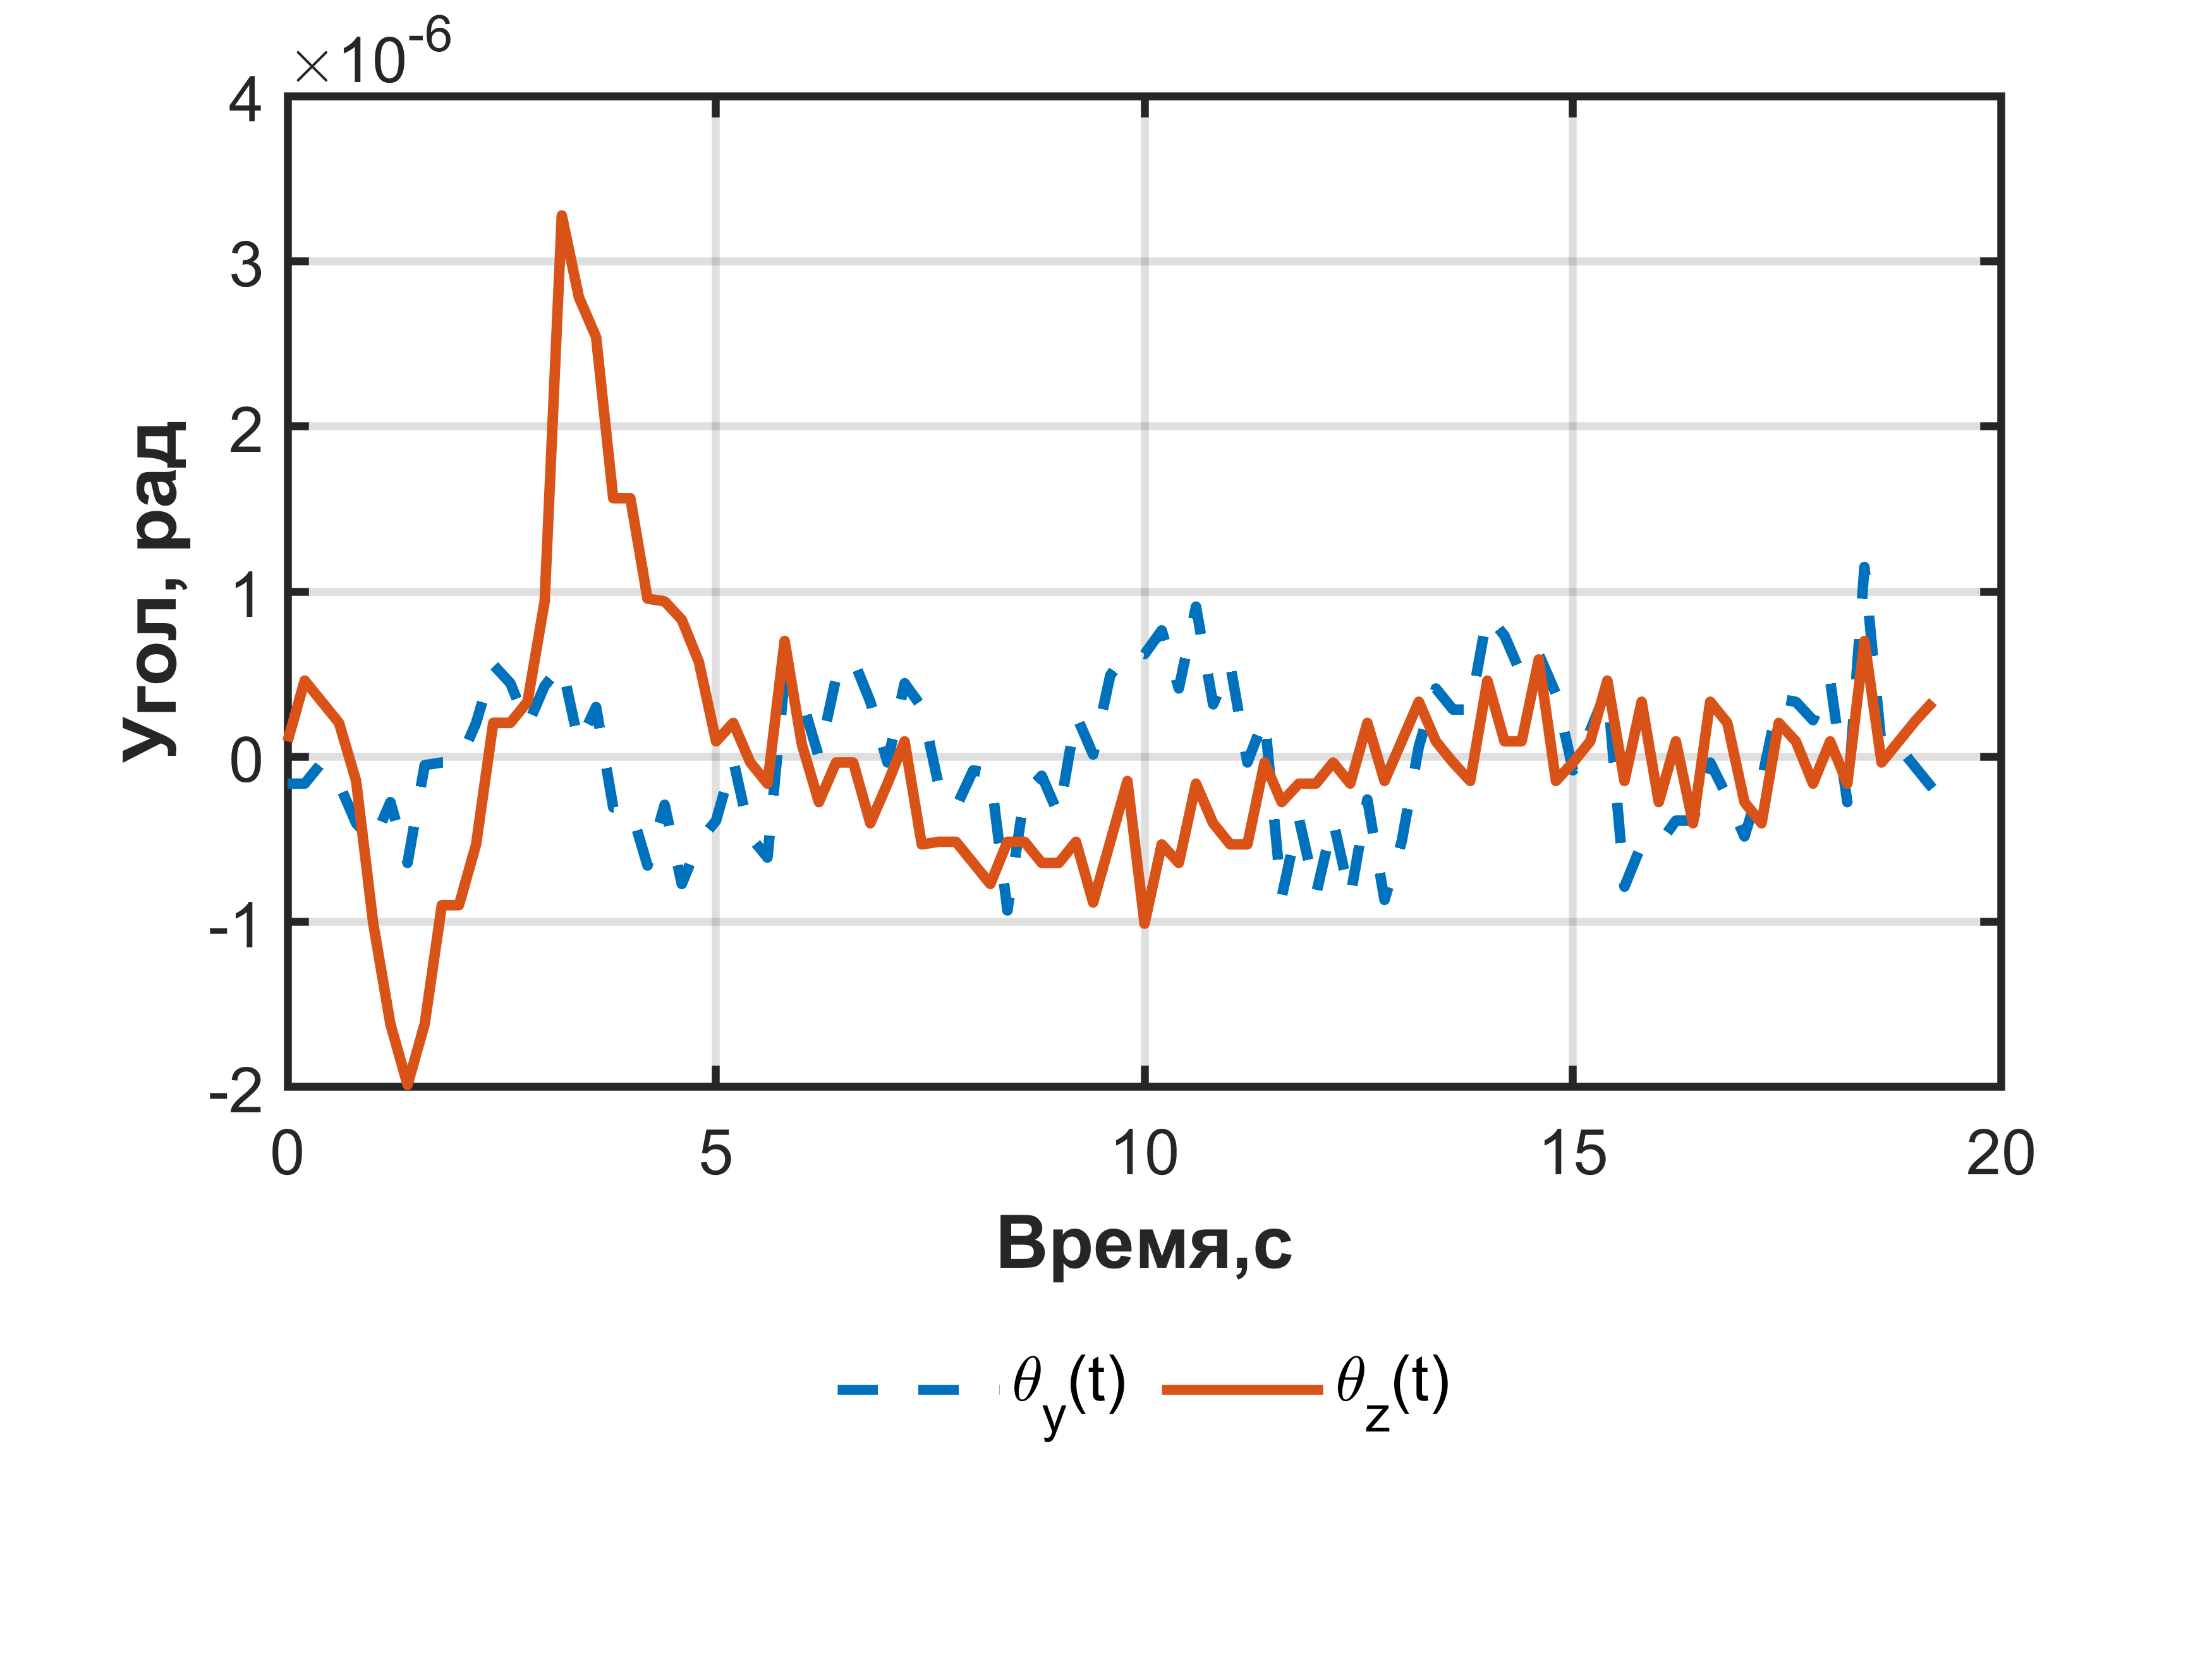
\includegraphics[width=1\linewidth]{matlab/img/thetaZ.png} \\ б)
 	\end{minipage}
 	\caption{Угловое перемещение спутника при повороте оси визирования по a) оси $OY$, б) оси $OZ$ }
 	\label{fig:theta}
 \end{figure}
 

 	Смещение изображения в фокальной плоскости определяется по формуле ~\eqref{eq:bias}, график показан на рисунке ~\ref{fig:bias}
 	
 	\begin{equation}
 		\label{eq:bias}
 		\mathbf{r}(t) = 
 		\begin{bmatrix}
 			y(t) \\
 			z(t) \\
 		\end{bmatrix}
 		= f \cdot
 		\begin{bmatrix}
 			\theta_{y}(t) \\
 			\theta_{z}(t)
 		\end{bmatrix}
 	\end{equation}
 	
 	где \(f=900000\) мкм --- фокусное расстояние
\newpage
 
 \begin{figure}[!h]
 	\begin{minipage}[b][][b]{0.49\linewidth}\centering
 		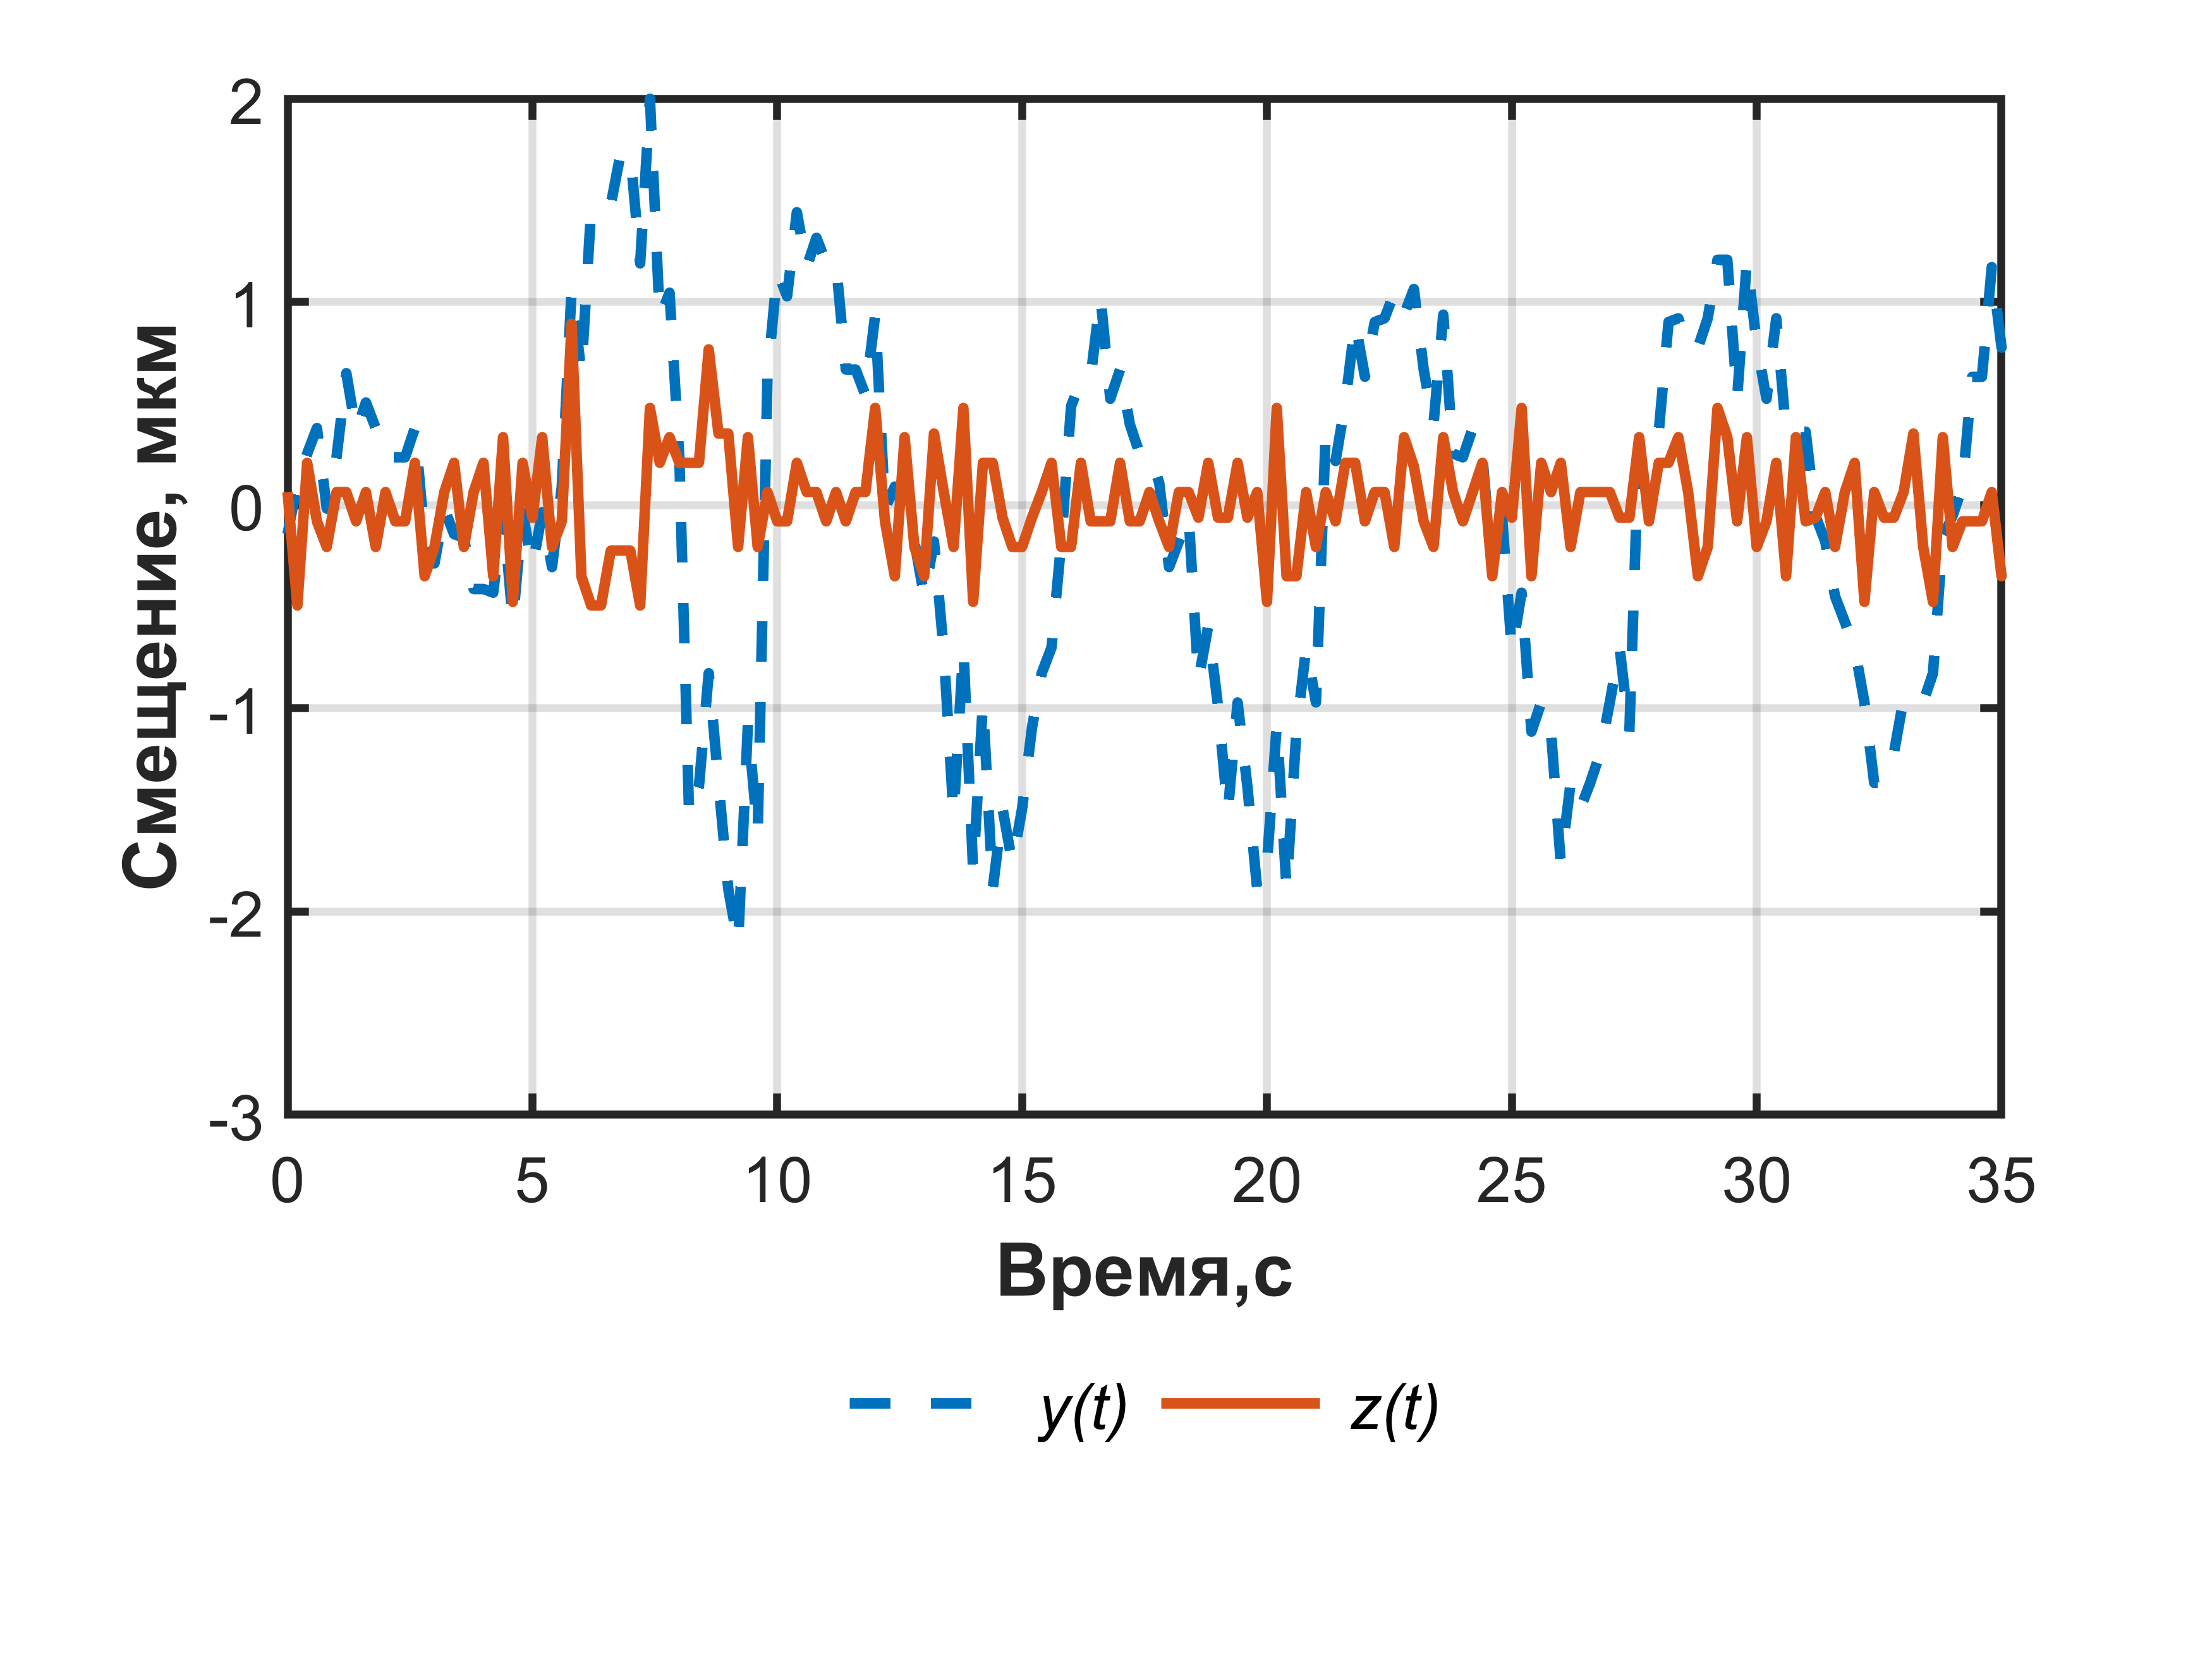
\includegraphics[width=1\linewidth]{matlab/img/biasY.png} \\ a)
 	\end{minipage}
 	\hfill
 	\begin{minipage}[b][][b]{0.49\linewidth}\centering
 		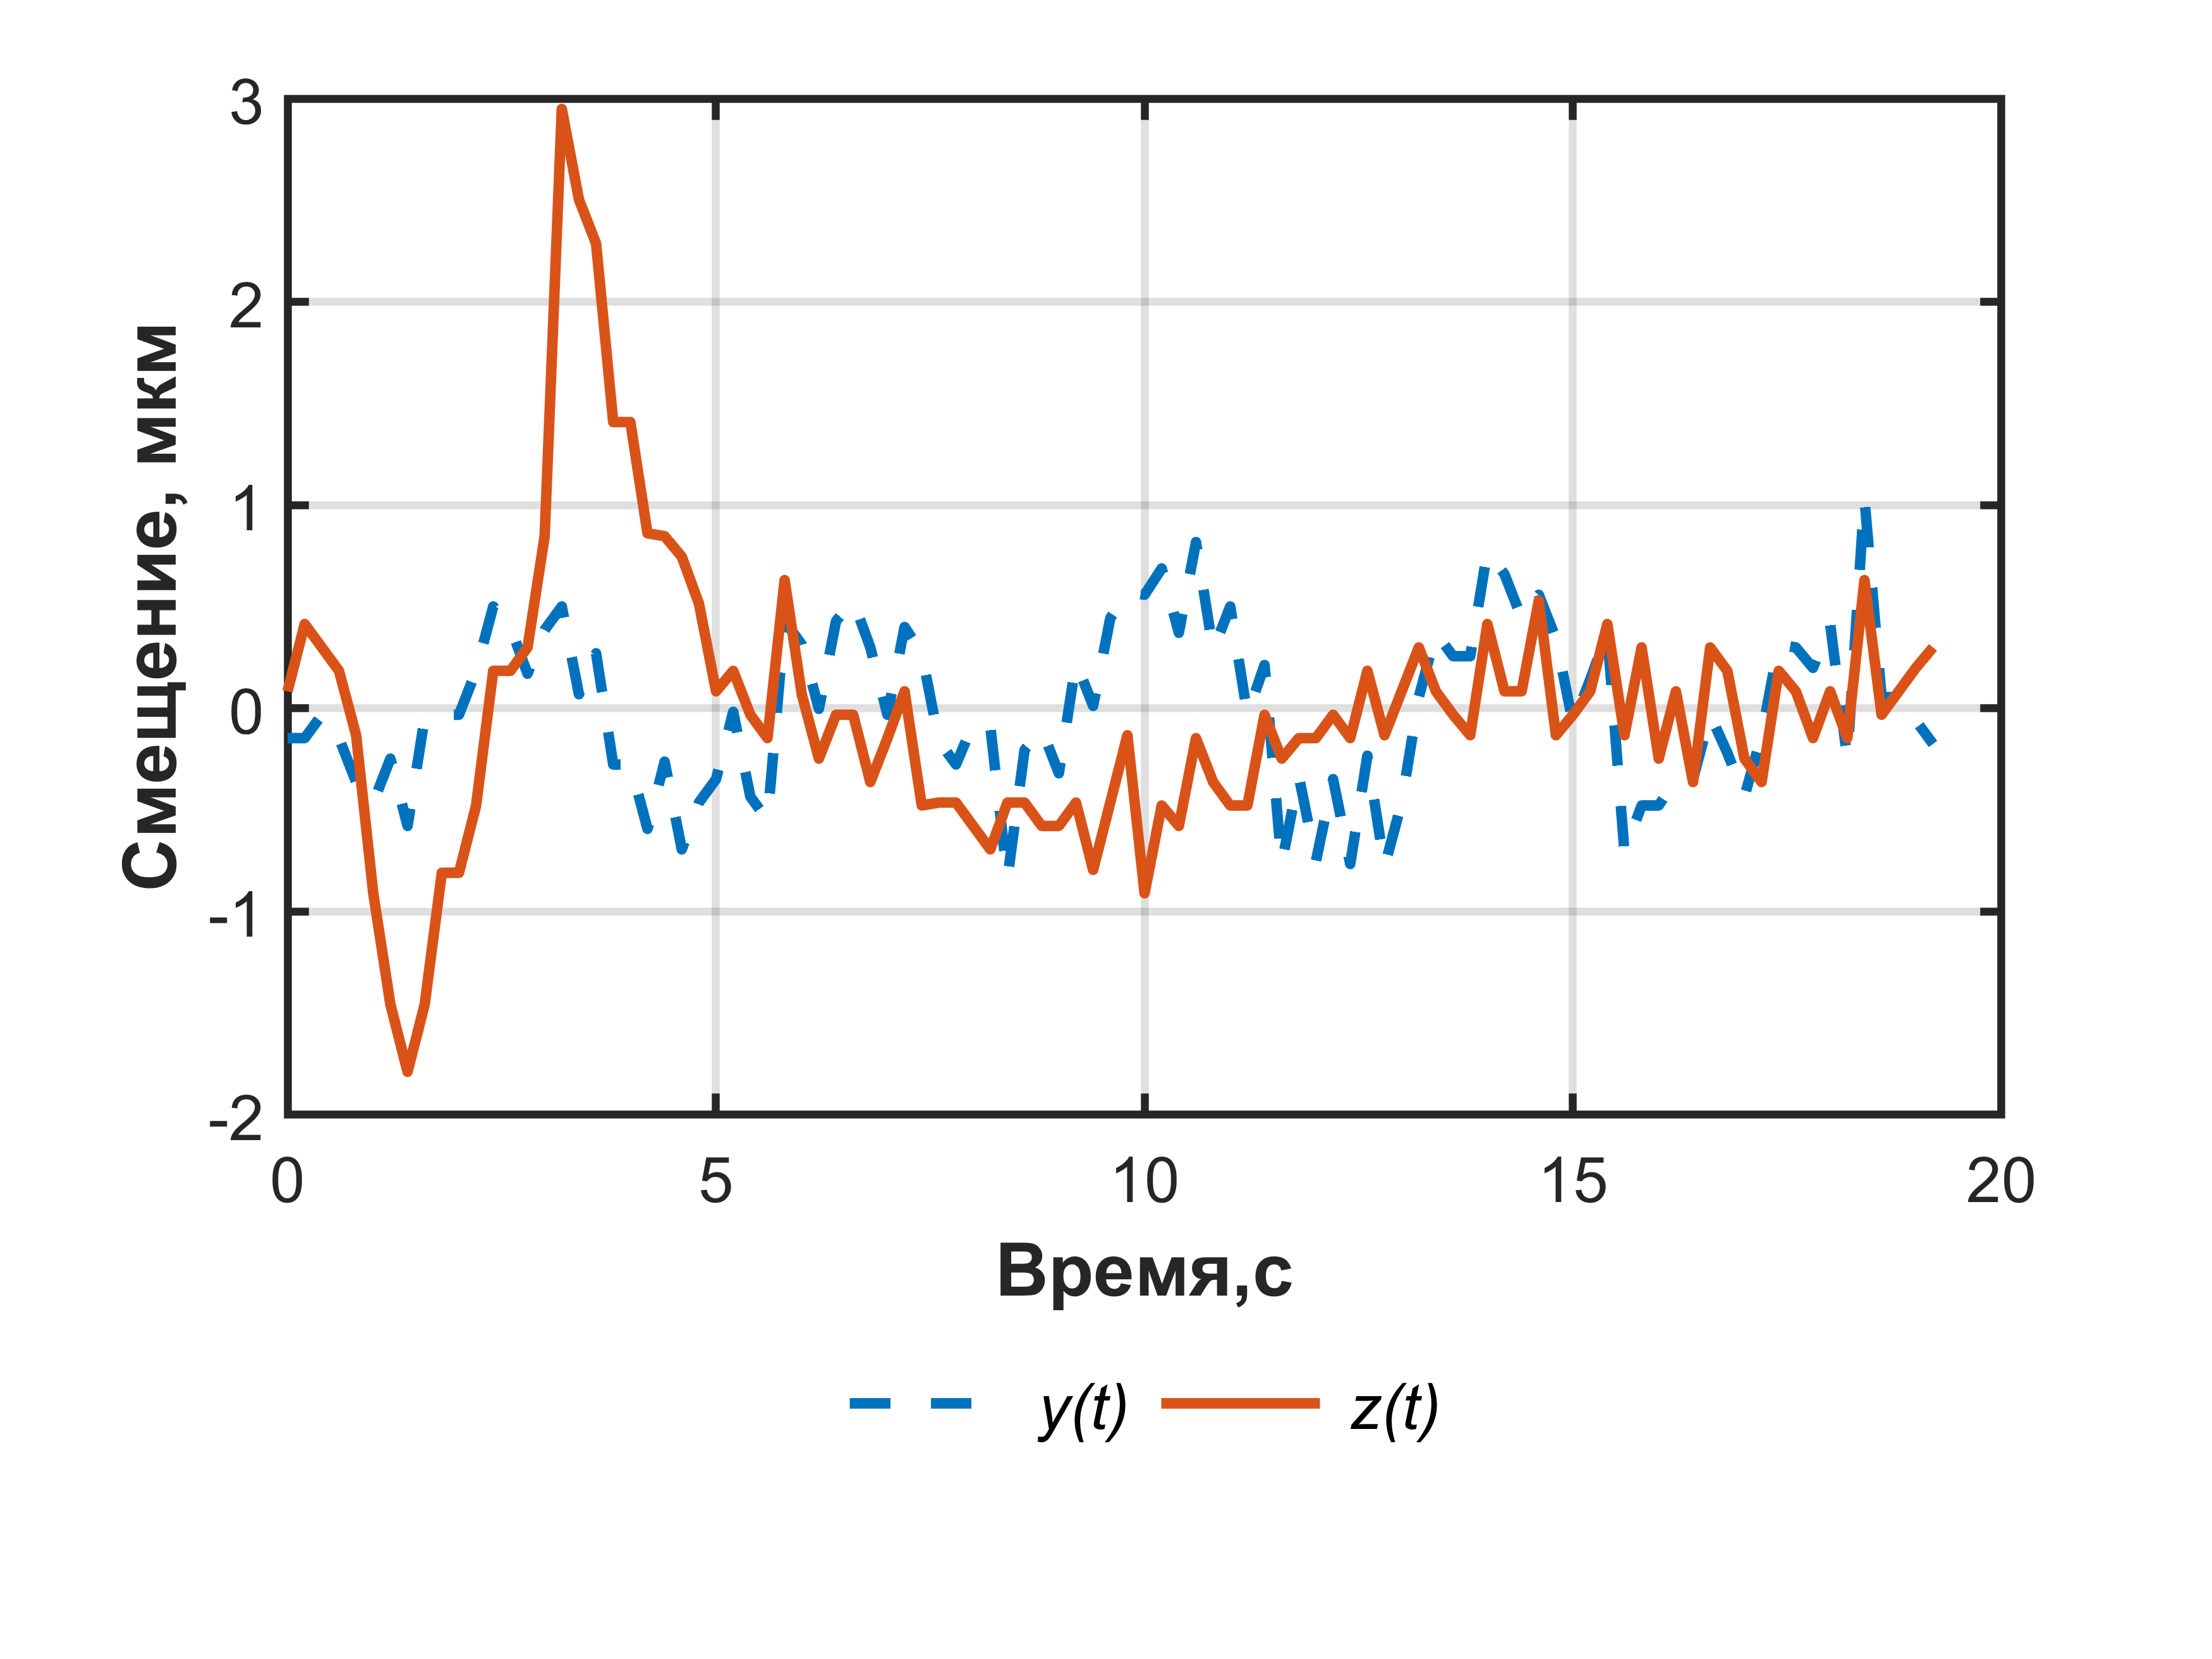
\includegraphics[width=1\linewidth]{matlab/img/biasZ.png} \\ б)
 	\end{minipage}
 	\caption{Смещение в фокальной плоскости при повороте оси визирования по a) оси $OY$, б) оси $OZ$ }
 	\label{fig:bias}
 \end{figure}
 
 
 За время экспозиции результирующий сдвиг имеет две составляющие: линейную~\eqref{eq:biasL} и угловую~\eqref{eq:rotate}.
 
 \begin{equation}
 	\label{eq:biasL}
 	L=\sqrt{(\Delta x)^2+(\Delta y)^2}
 \end{equation}
 
 \begin{equation}
 	\label{eq:rotate}
 	\alpha = R \cdot \theta_x
 \end{equation}
 
 
 Для оценки влияния на качество изображения используется суммарная длина \blur{а} как векторная сумма линейной и угловой составляющих:
 
 \begin{equation}
 	\label{eq:L_total}
 	L = \sqrt{L^2 + (R\cdot \theta_x)^2 + 2Lr\theta_x\cos{\psi}}
 \end{equation}
 
 где \(\psi\) -- угол между векторами направлений \blur{а}
 
 
 \begin{figure}[!h]
 	\begin{minipage}[b][][b]{0.49\linewidth}\centering
 		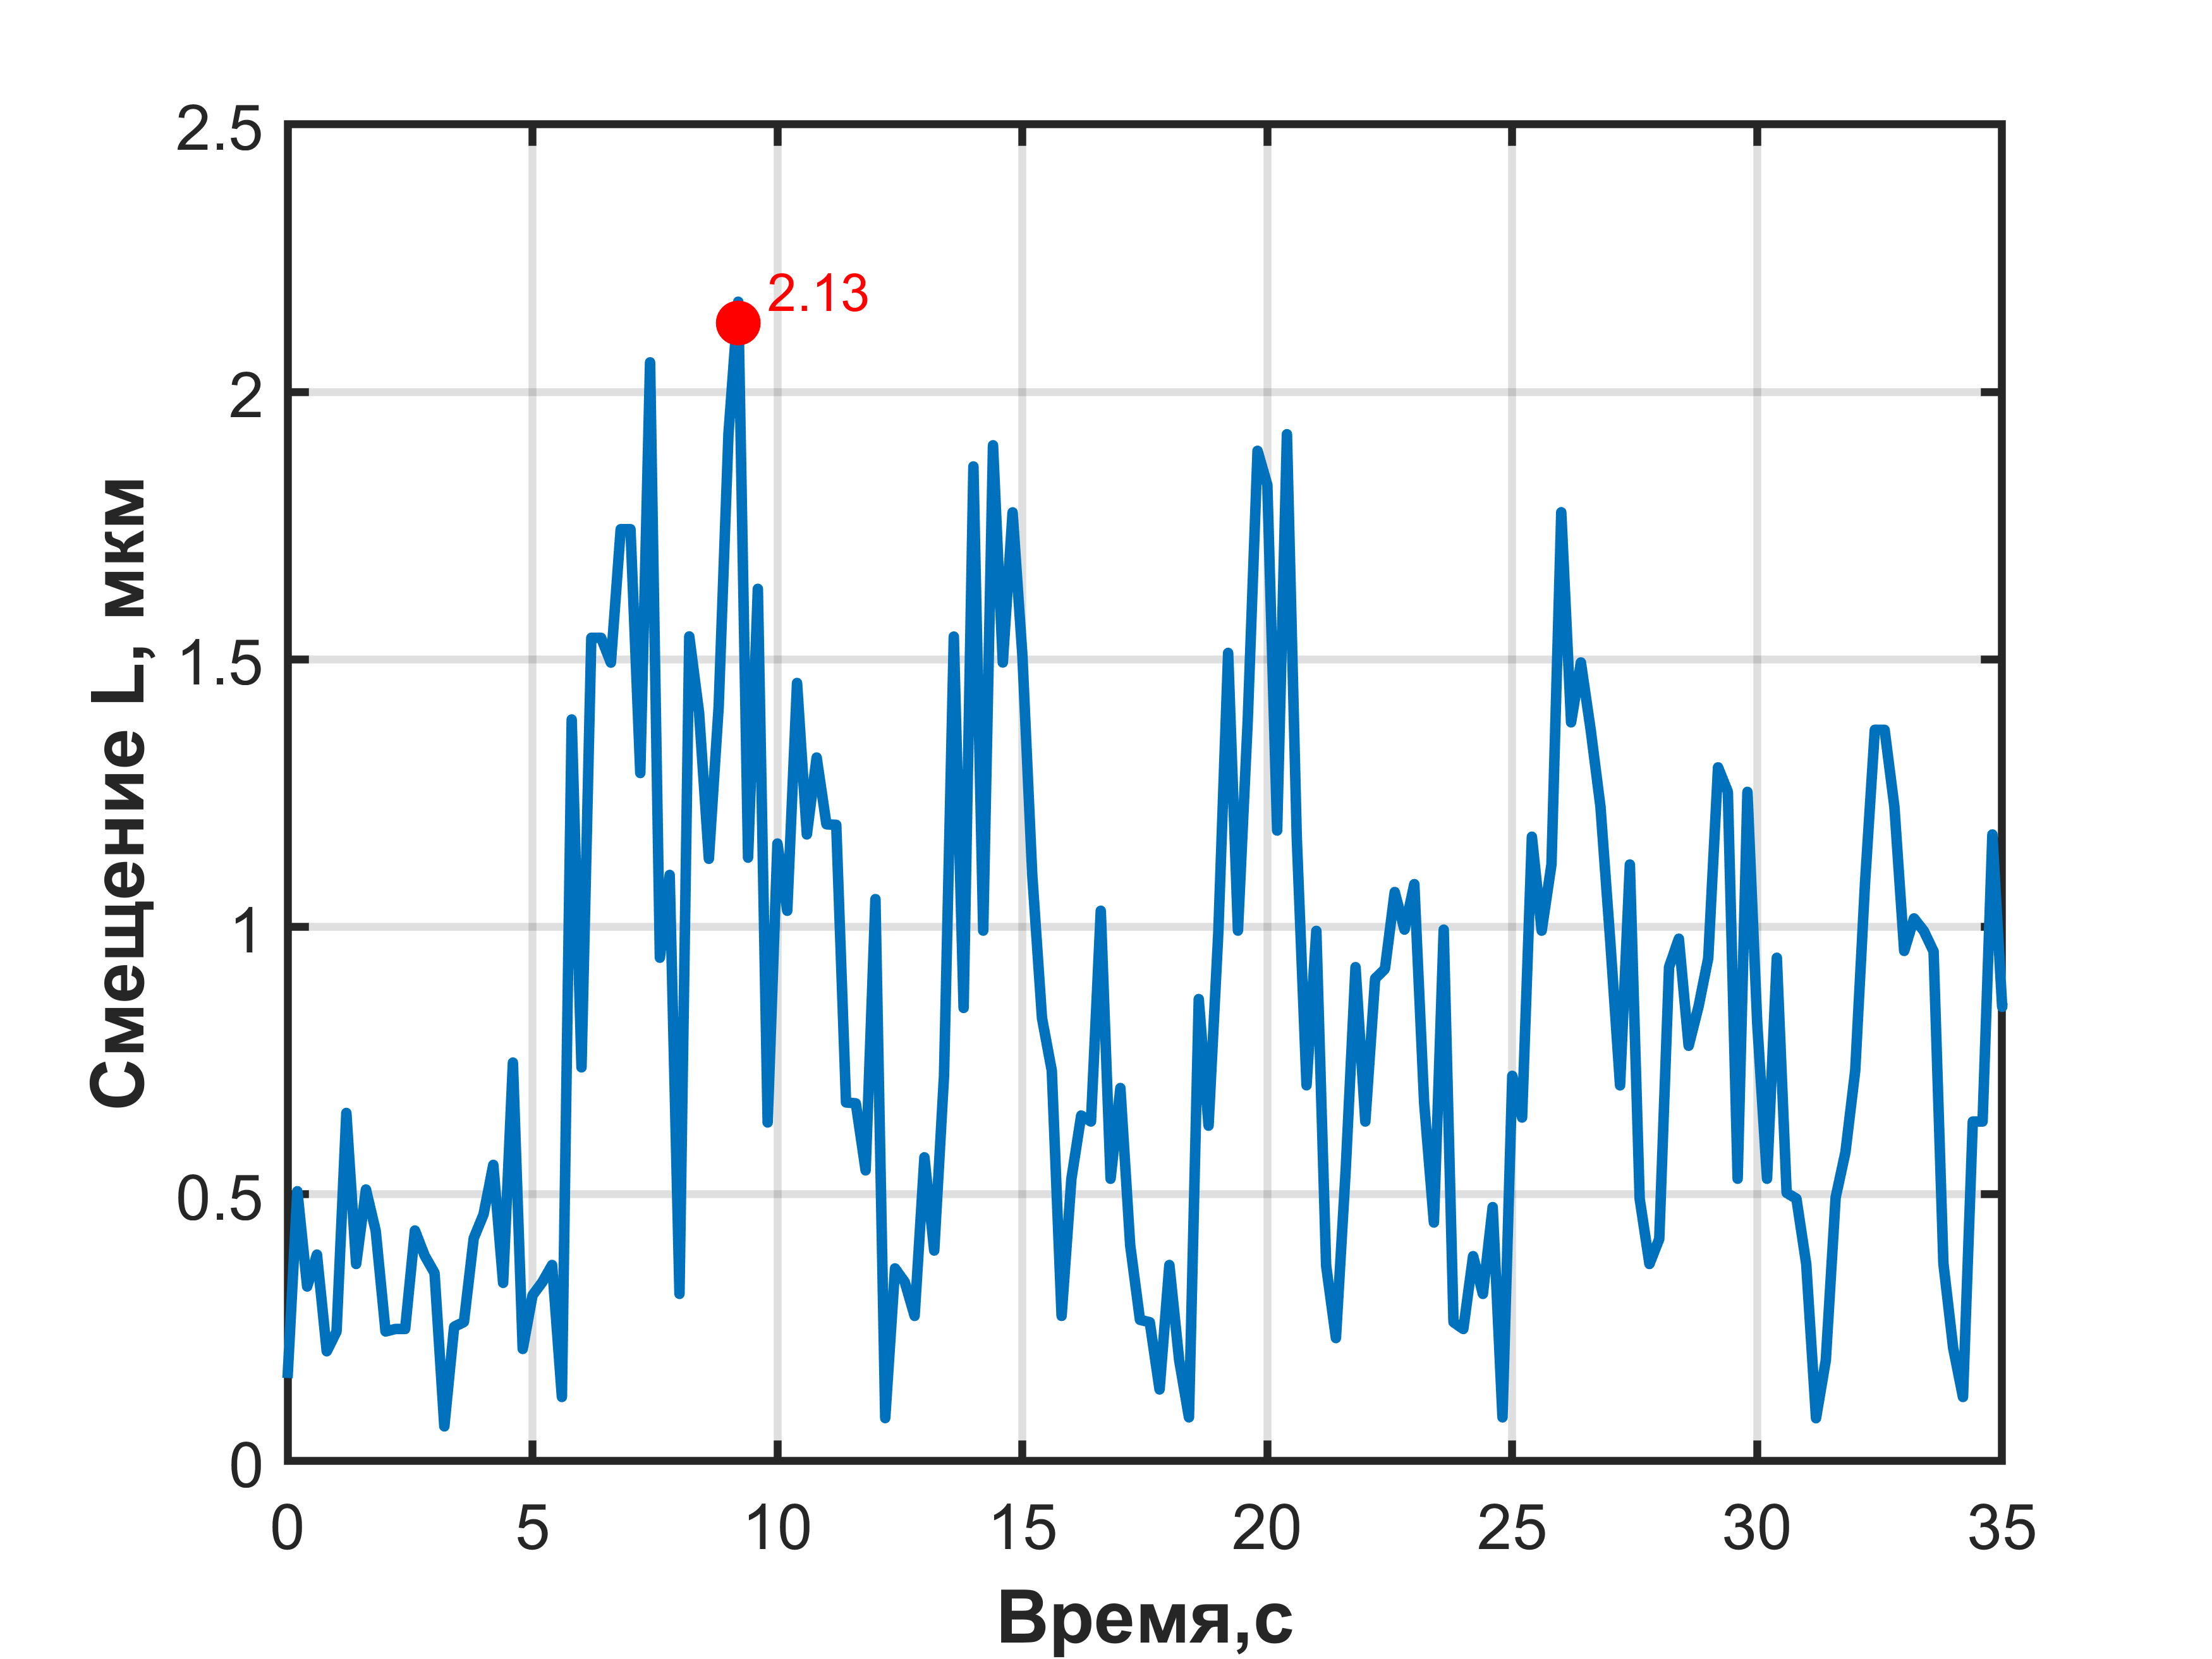
\includegraphics[width=1\linewidth]{matlab/img/LmaxY.png} \\ a)
 	\end{minipage}
 	\hfill
 	\begin{minipage}[b][][b]{0.49\linewidth}\centering
 		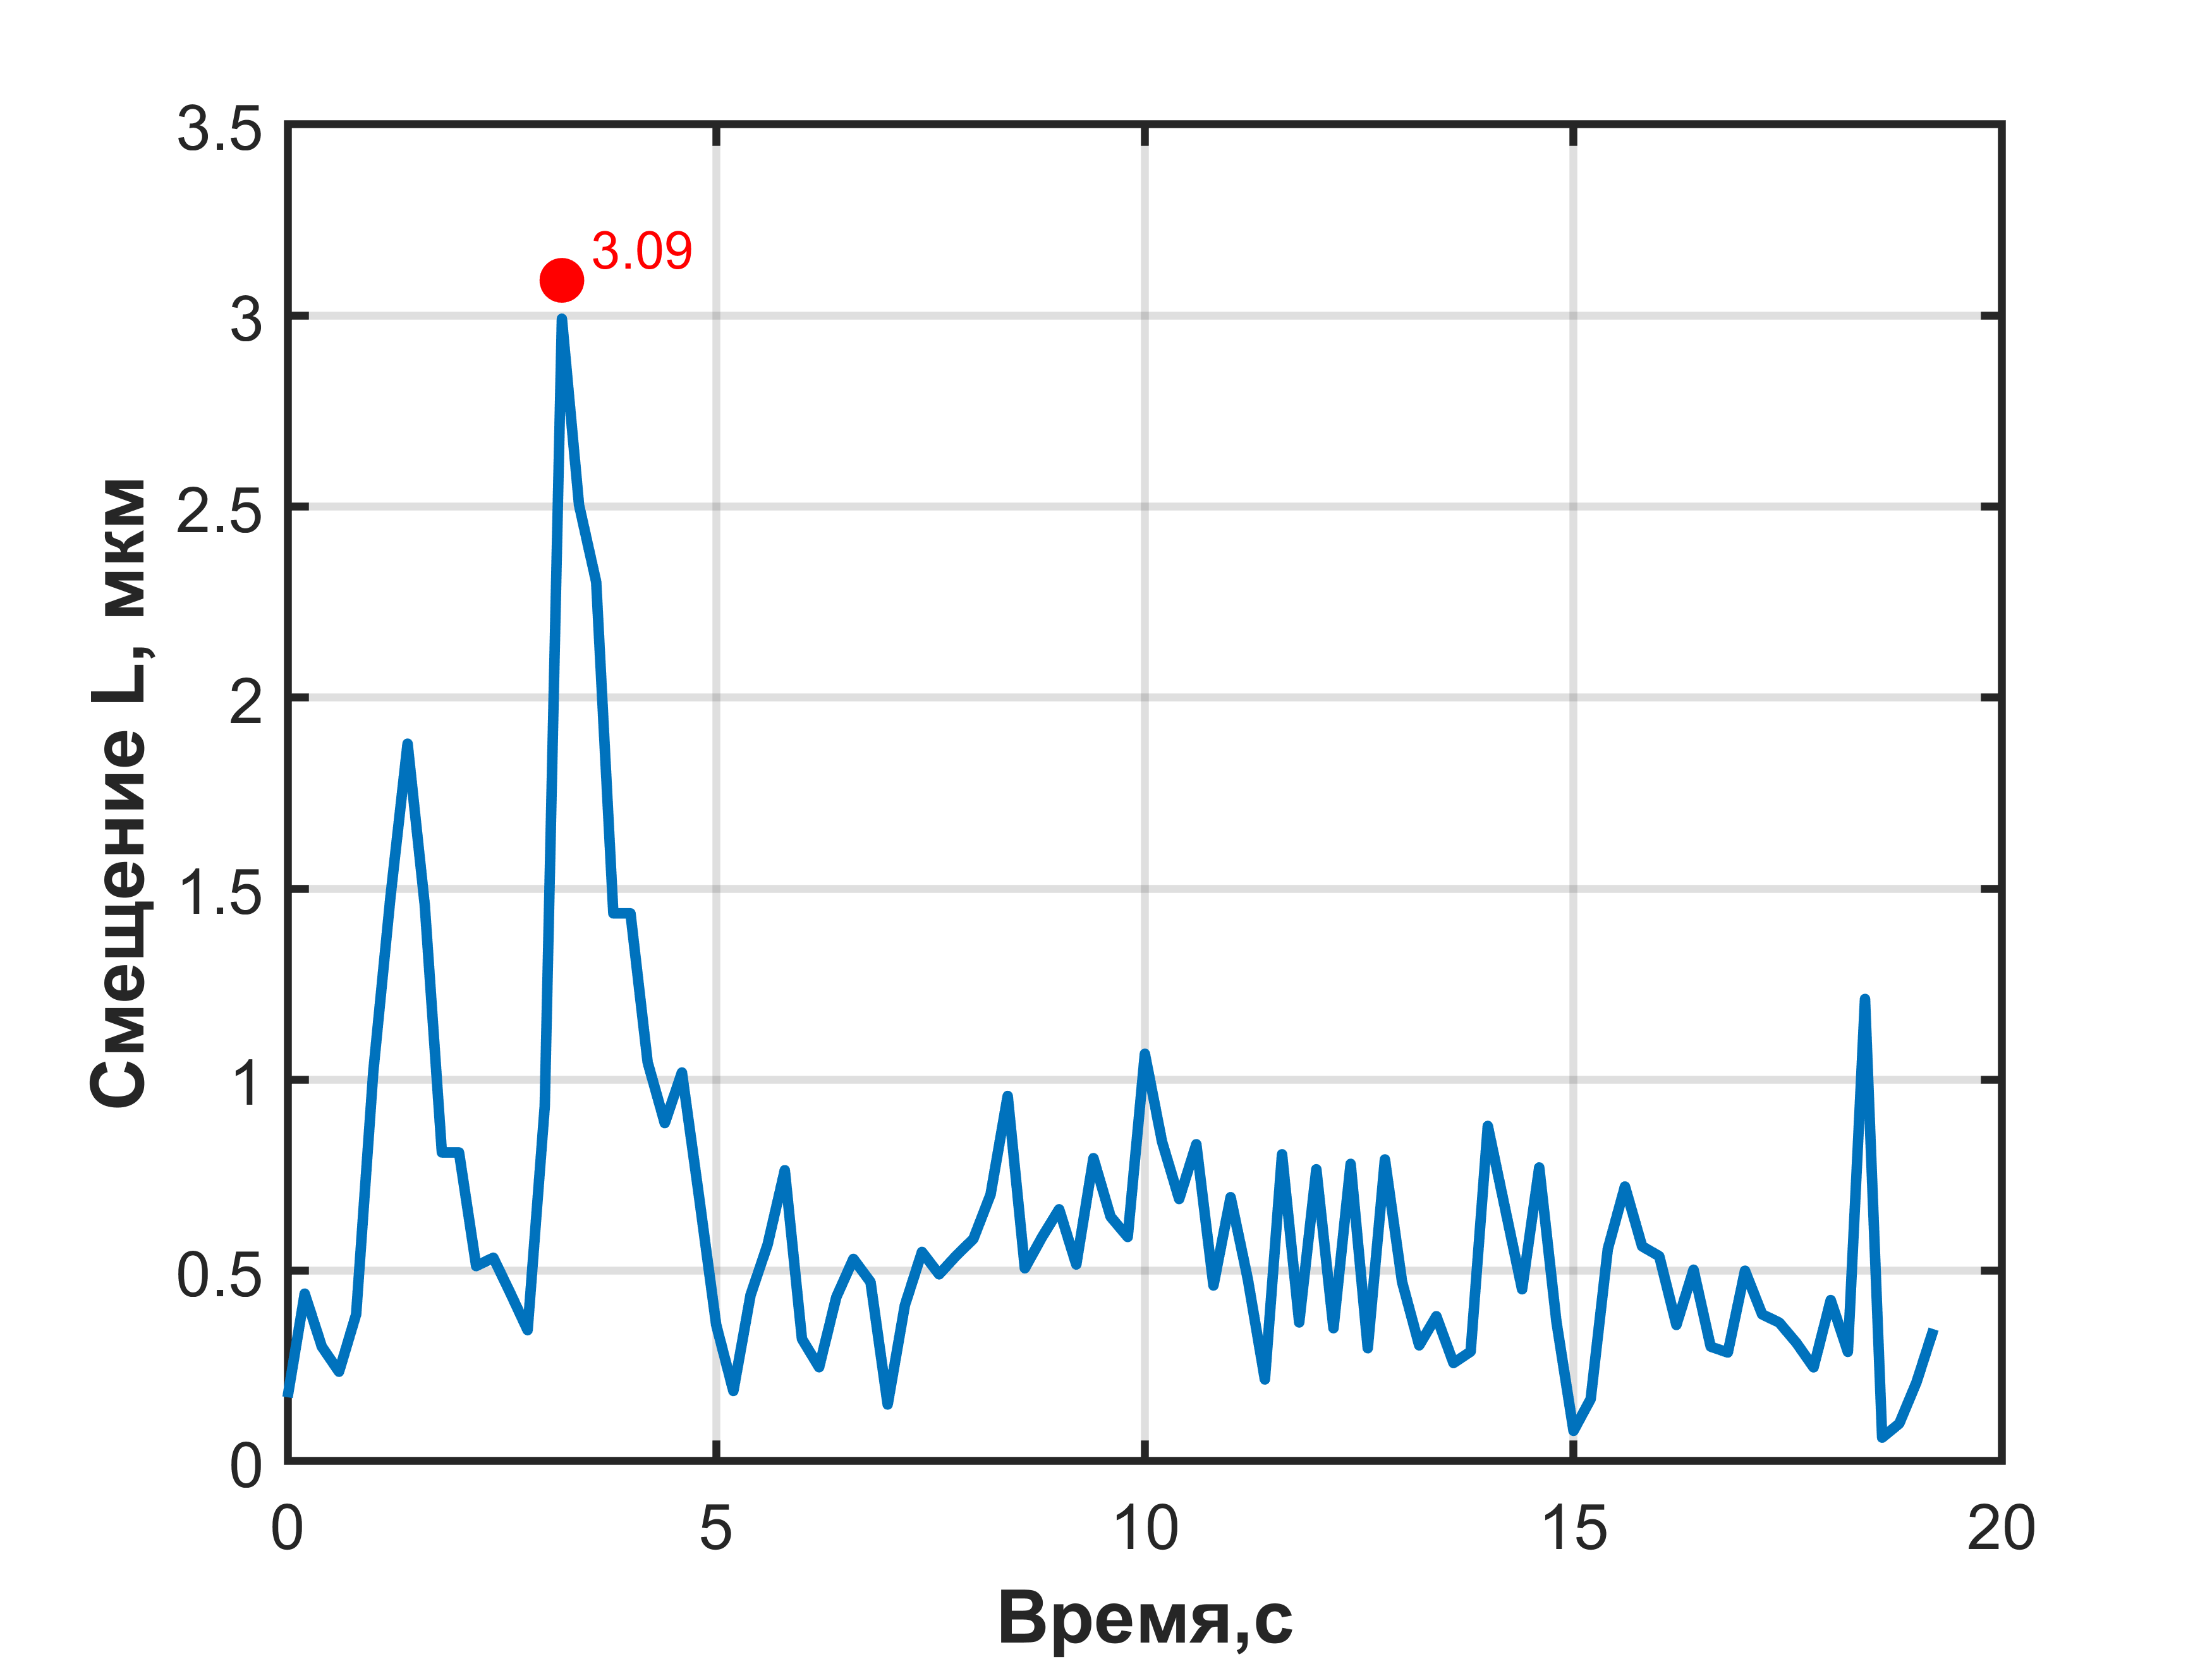
\includegraphics[width=1\linewidth]{matlab/img/LmaxZ.png} \\ б)
 	\end{minipage}
 	\caption{Полное смещение в фокальной плоскости при повороте оси визирования по a) оси $OY$, б) оси $OZ$ }
 	\label{fig:biasL}
 \end{figure}
 
 Траектория сдвига в пределах экспозиции квазипрямолинейна, поэтому деградация ФПМ вдоль худшего направления описывается аппроксимацией линейного размытия:
 
 \begin{equation}
 	\label{eq:MTF_aprox}
 	MTF(\nu) = \frac{\sin\!\bigl(\pi \nu L\bigr)}{\pi \nu L}
 \end{equation}
 
 где \(\nu\) -- частота Найквиста по дискретизации, определяется следующим образом:
 
 \begin{equation}
 	\label{eq:nykvist}
 	\nu = \frac{1}{2p} \approx \SI{16.7}{\per\milli\meter}
 \end{equation}
 где \(p\) --- размер пикселя, в исследуемой системе составляет \SI{30}{\micro\meter}
 
 Согласно рассчитанным траекториям (см. рисунок ~\ref{fig:biasL}), максимальная величина результирующего смещения изображения за время экспозиции:
 \begin{enumerate}
 	\item поворот вокруг $OY$: $L= \SI{2,13}{\micro\meter}$
 	\item поворот вокруг $OZ$: $L= \SI{3,09}{\micro\meter}$
 \end{enumerate}
 
 В относительных единицах это соответствует:
 \begin{equation}
 	\frac{L_{OY}}{p} \approx 0,07 \quad \quad \frac{L_{OZ}}{p} \approx 0,1
 \end{equation}
 
 На предельной частоте дискретизации $\nu = \nu_N$ получаем:
 
 \begin{equation}
 	\begin{split}
 		\label{eq:MTF_result}
 		MTF(\nu_N)_{OY}=\frac{\sin\!\bigl(\pi \nu_N L\bigr)}{\pi \nu_N L} =  \frac{\sin\!\bigl(\pi \cdot 16,7 \cdot 0,00213 \bigr)}{\pi 16,7 \cdot 0,00213} \approx  0,9979\\
 		MTF(\nu_N)_{OZ}=\frac{\sin\!\bigl(\pi \nu_N L\bigr)}{\pi \nu_N L} =  \frac{\sin\!\bigl(\pi \cdot 16,7 \cdot 0,00309 \bigr)}{\pi \cdot 16,7 \cdot 0,00309} \approx 0,9956
 	\end{split}
 \end{equation}
 
Таким образом, проведённые расчёты подтвердили, что остаточный реактивный момент после реализации мероприятий по компенсации не оказывает критического влияния на формирование изображения. Полученные результаты согласуются с предварительными стендовыми испытаниями и подтверждают достоверность выбранного подхода к компенсации динамических возмущений.
 
 \section{Применение стенда для испытаний других оптических систем}
 
 Разработанный стенд был использован не только для исследования оптико-механического модуля с дискретными поворотами, но и для испытаний системы с иным принципом работы. В данном случае объектом исследований являлась оптическая система, в которой блок зеркал совершает постоянные периодические колебательные движения. Для подобных систем предъявляются более жёсткие требования к уровню остаточного реактивного момента: он не должен превышать $\SI{0,005}{\newton\meter}$. 
 
 Особенностью конструкции является наличие компенсационного маховика, управляемого отдельным электродвигателем. Для эффективного подавления реактивного момента требуется высокая точность согласования работы двигателя нагрузки и двигателя компенсационного маховика.
 
 \begin{figure}[h!]
 	\centering
 	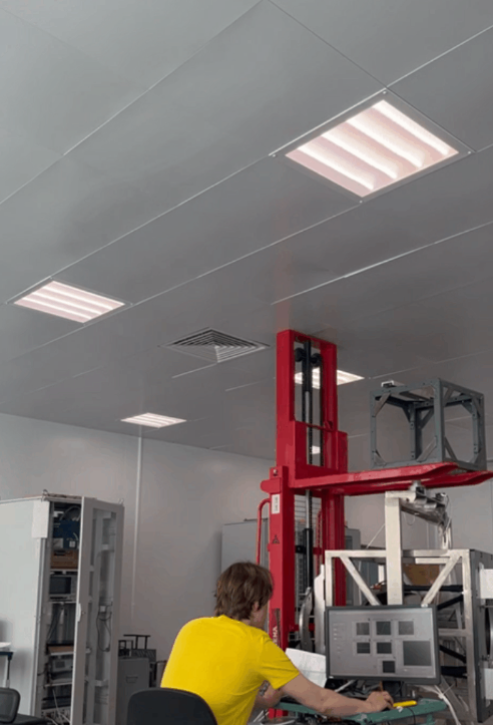
\includegraphics[scale=0.8]{images/scaner-stand}
 	\caption{Проведение измерений реактивного момента ОМС}
 	\label{fig:scan-stand}
 \end{figure}
 
 Испытания проводились на стенде в несколько этапов. На первом этапе выполнялся эмпирический подбор момента инерции компенсационного маховика: его конструкция предусматривала возможность «вручную» добавлять или убирать кольца, изменяя тем самым величину момента инерции. После определения оптимального значения инерции переходили ко второму этапу — синхронизации работы двигателей нагрузки и компенсационного маховика. Для этого параметры управления подбирались экспериментально до достижения устойчивого совпадения фаз их колебаний, что обеспечивало минимизацию остаточного реактивного момента. 
 
 На рисунке~\cref{fig:scan-mom} показаны результаты измерений: реактивный момент оптической системы до и после настройки.
 
 \begin{figure}[h!]
 	\begin{minipage}[b]{0.49\linewidth}\centering
 		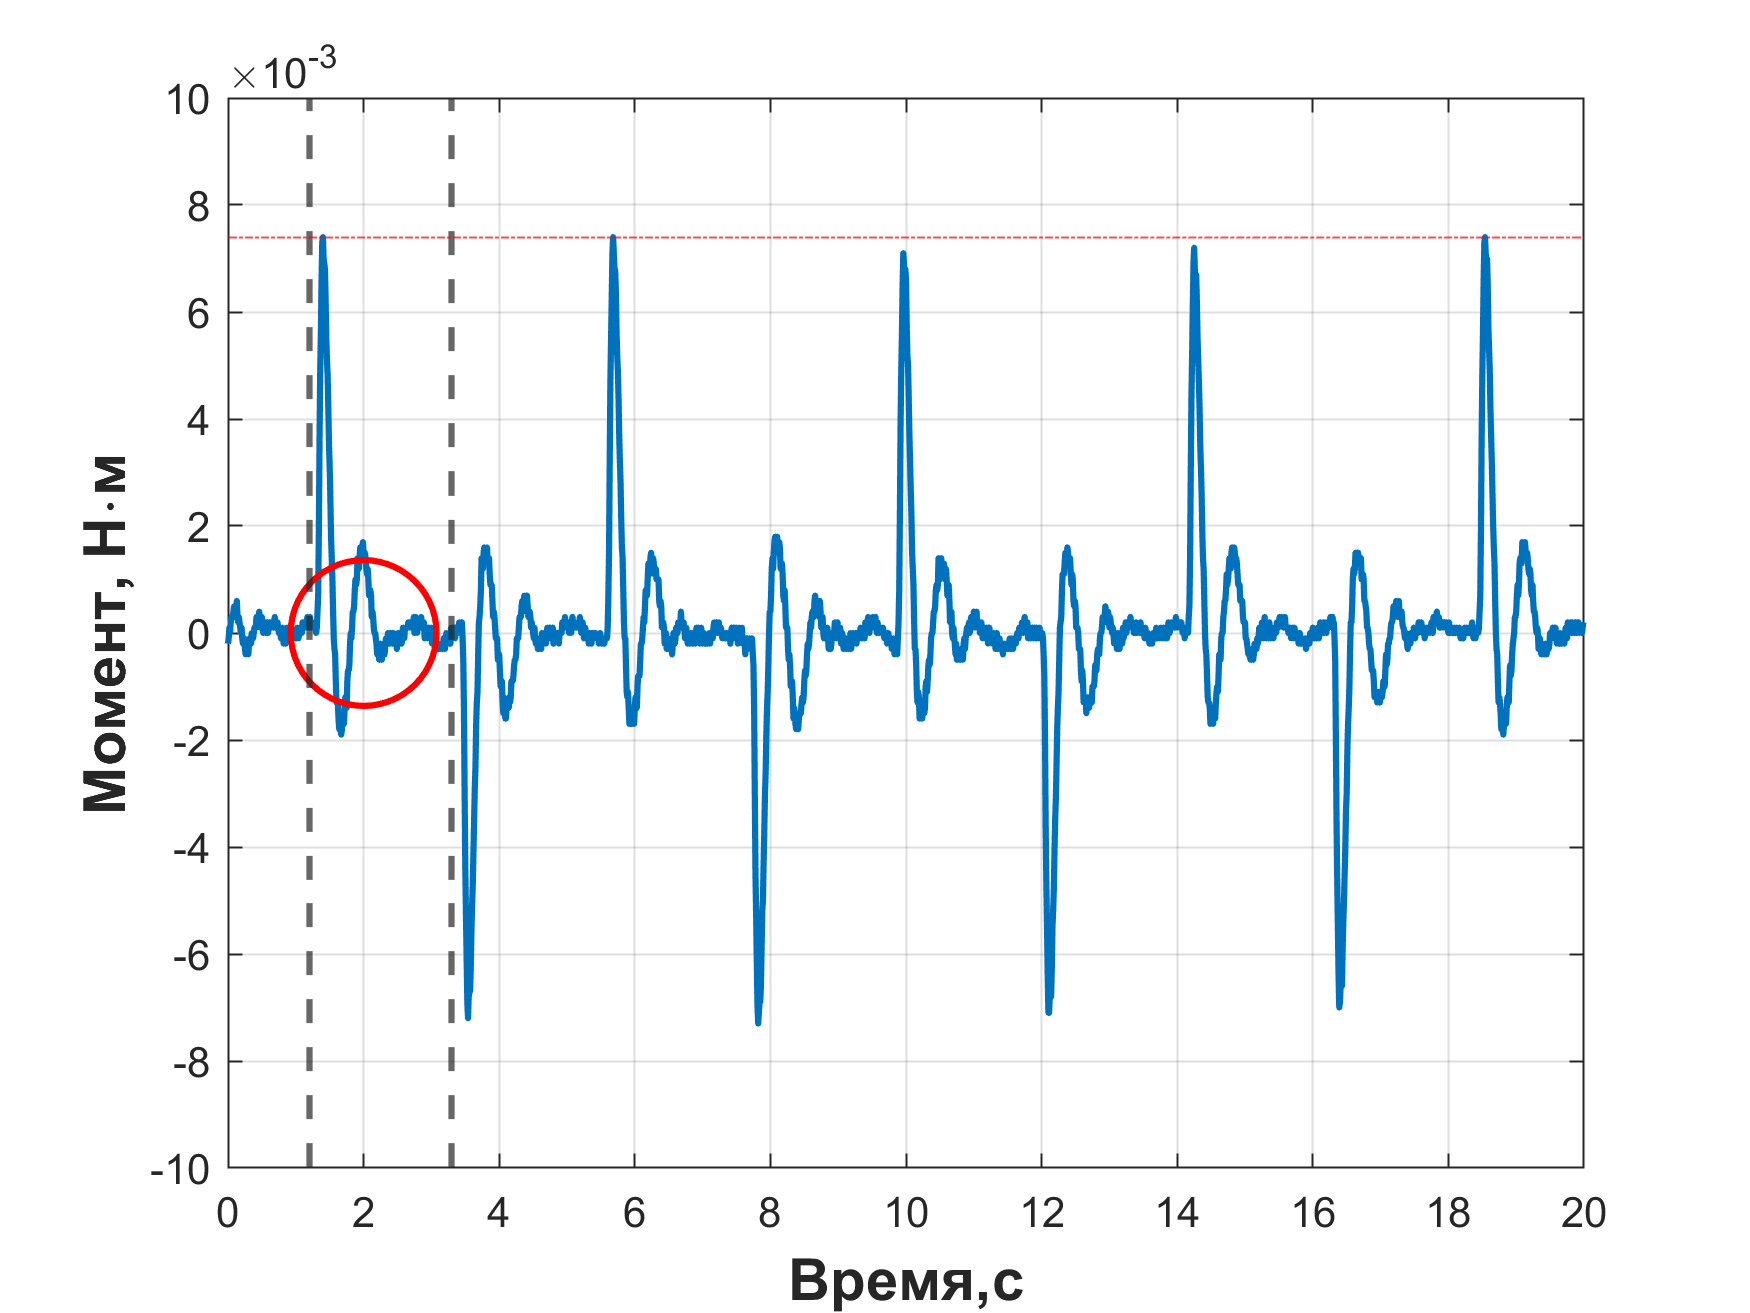
\includegraphics[width=1\linewidth]{matlab/img/scanner_no_sinchron} \\ а)
 	\end{minipage}
 	\hfill
 	\begin{minipage}[b]{0.49\linewidth}\centering
 		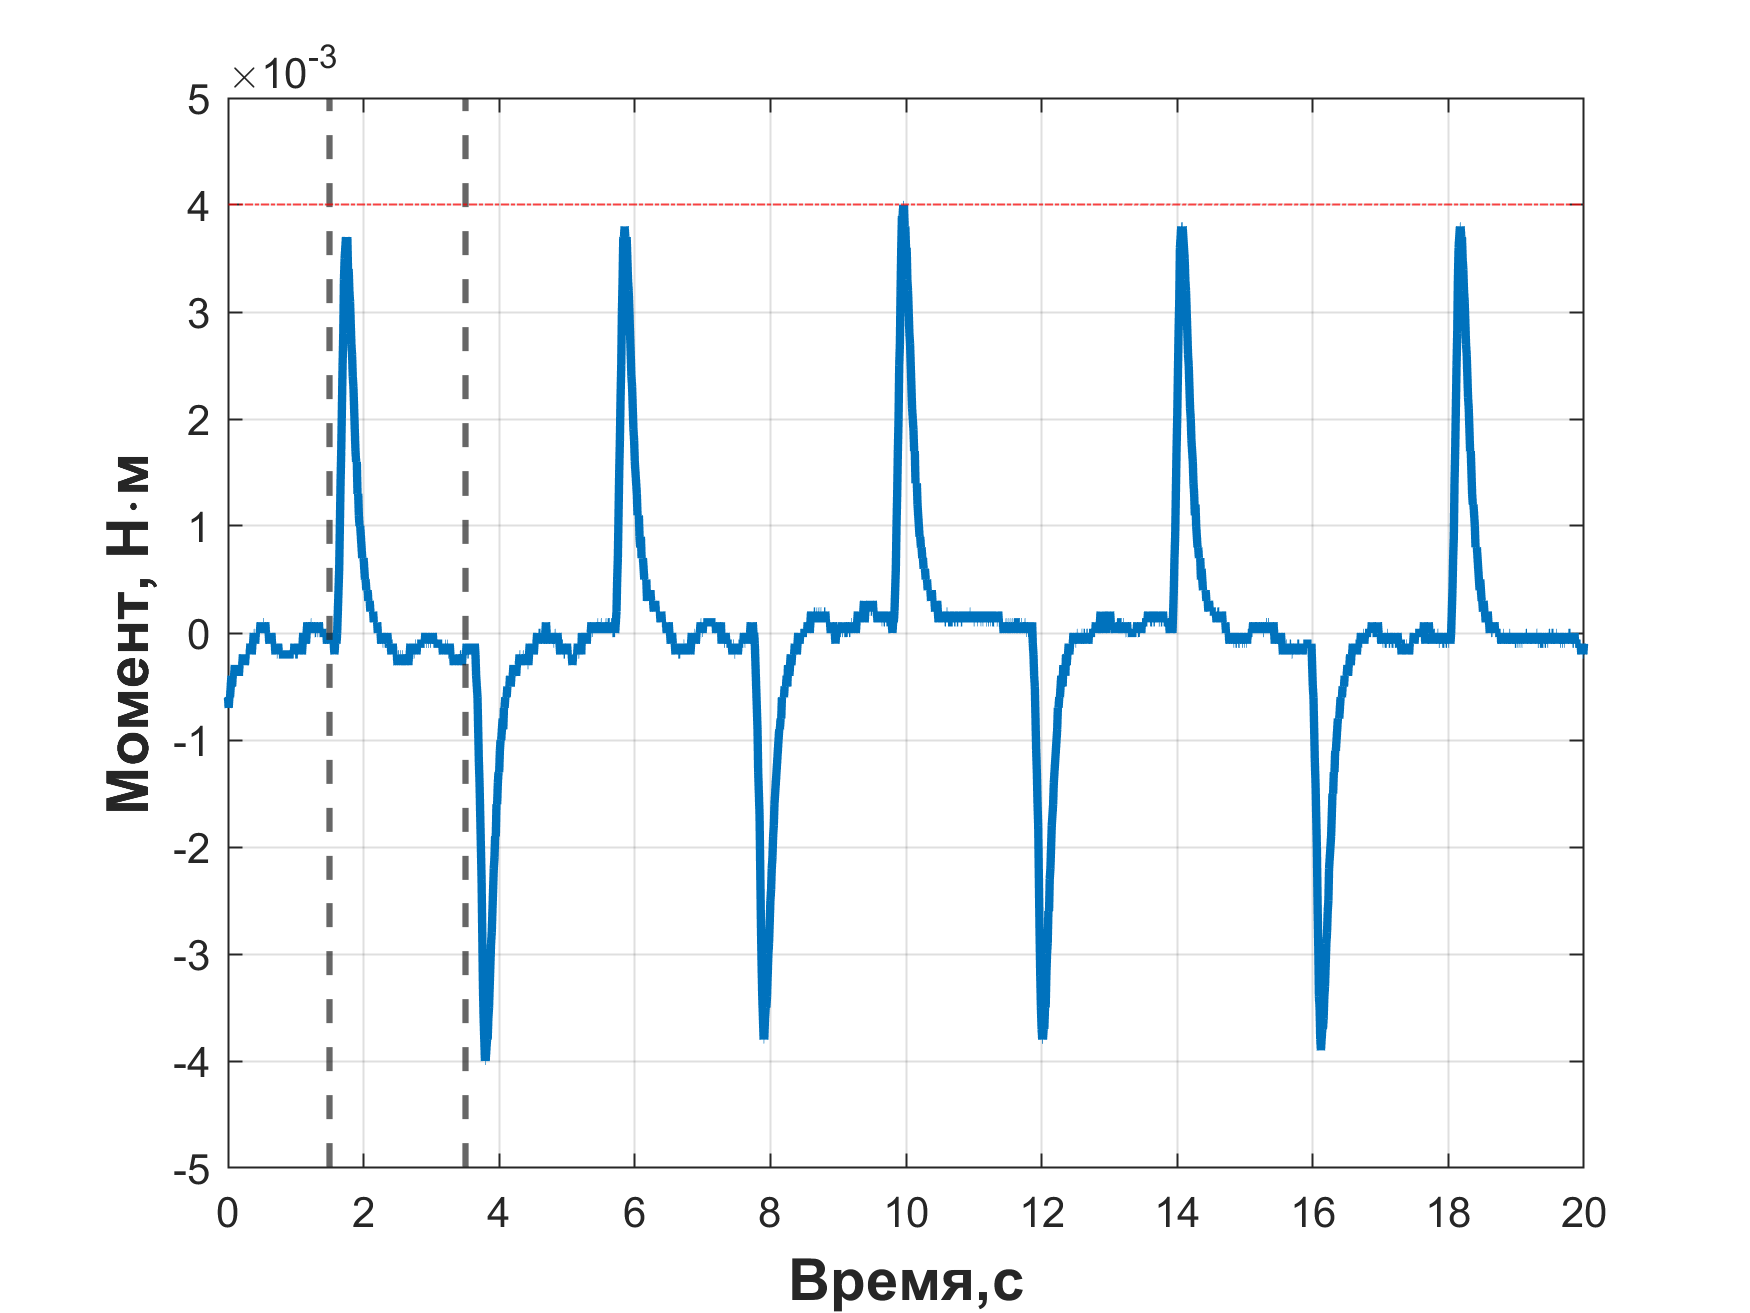
\includegraphics[width=1\linewidth]{matlab/img/scanner_correct} \\ б)
 	\end{minipage}
 	\caption{Реактивный момент оптической системы: а) до настройки; б) после настройки}
 	\label{fig:scan-mom}
 \end{figure}
 

 Таким образом, проведённые испытания подтвердили эффективность предложенной методики. Она позволяет не только уменьшить уровень остаточного реактивного момента до наилучшего значения, но и обеспечивает возможность настройки синхронной работы приводов в оптико-механических системах с колебательными элементами. Полученные результаты показывают, что методика может быть применена и для других типов оптических систем, где требуется высокая динамическая точность и минимизация возмущающих воздействий.
 
 
 \section*{Выводы по главе 4}
 
В четвёртой главе выполнена экспериментальная проверка предложенной методики измерения остаточного реактивного момента. Результаты испытаний показали хорошее совпадение с расчётными данными, полученными во второй главе: при повороте МНО вокруг осей $OY$ и $OZ$ зарегистрированы моменты $M_y = \SI{0,076}{\newton\meter}$ и $M_z=\SI{0,055}{\newton\meter}$, что подтверждает корректность разработанного подхода.

Для повышения эффективности компенсации были рассчитаны и установлены балансировочные кольца на маховики, после чего проведена повторная серия стендовых экспериментов с использованием синусоидального профиля управления приводом. Измерения показали снижение величины реактивного момента, более плавный характер переходных процессов и уменьшение возбуждения колебаний подвесной системы. 

Достоверность результатов стендовых испытаний подтверждена анализом данных бортовых гироскопов лётного образца. Определённые по телеметрии угловые перемещения позволили оценить смещение изображения в фокальной плоскости. Максимальные значения линейного сдвига составили $L_{OY} = \SI{2,13}{\micro\meter}$ и $L_{OZ} = \SI{3,09}{\micro\meter}$, что соответствует $0,07$ и $0,10$ пикселя при размере элемента $\SI{30}{\micro\meter}$.
Расчёт функции передачи модуляции показал, что остаточный реактивный момент приводит к уменьшению 
$MTF$ на частоте Найквиста лишь до $0,995-0,998$, то есть не оказывает существенного влияния на качество изображения.
 
Кроме того, показано, что разработанный стенд может применяться и для отработки оптических систем с колебательными элементами. В таких случаях методика позволяет экспериментально подобрать инерцию компенсационного маховика и синхронизировать работу приводов, обеспечивая снижение остаточного реактивного момента до требуемого уровня.

Таким образом, проведённые исследования подтвердили эффективность предложенной методики как для оценки, так и для практической компенсации реактивных моментов в различных типах оптико-механических систем.
 
 
\FloatBarrier




